\documentclass[ xcolor = pdftex, dvipsnames, table ]{beamer}

\usetheme[compress]{Berlin}
\usecolortheme{whale}
\setlength{\parskip}{0.1in}
\usepackage{bm}
\usepackage{color}
\usepackage{graphicx}
%\usepackage[percent]{overpic}
\usepackage{xcolor}
\usepackage{tikz}
%\usepackage[makeroom]{cancel}
\usetikzlibrary{positioning, shapes, snakes}

%
%

\begin{document}

%
%ftp://ftp.pcouncil.org/pub/!!!Catch_Estimation_Methodology_Review_2018/

\title{\textbf{Improving Catch Estimation Methods in Sparsely Sampled, Mixed Stock Fisheries.}}

\author{
\textbf{\mbox{Nick Grunloh}}
%%$~$\\
%%\vspace{-0.5cm}
%\textbf{Nicholas Grunloh, }\\%\vspace{0.3cm}
%%\textbf{In Cooperation With:}\\
%\textbf{E.J. Dick, Don Pearson, John Field, Marc Mangel}
}

\institute[]{\textbf{UCSC :: CSTAR :: SWFSC :: NMFS}}

%\logo{
%\includegraphics[width=0.75\textwidth]{./Rockfish.png}
%}

%\institute{Foo Research Institution\\
%      \includegraphics[width=0.05\textwidth]{./Rockfish.png}
%}

\date{
%$~$\\
%\vspace{-1.5cm}
%\includegraphics[width=0.45\textwidth]{./Rockfish.png}\\
\textbf{28 March 2018}
}

%
%

%
\section{Introduction}
\subsection{}
\begin{frame}
	\maketitle
\end{frame}

%
%

%
\subsection{}
\begin{frame}
\centering
$~$\\
\vspace{-0.5cm}
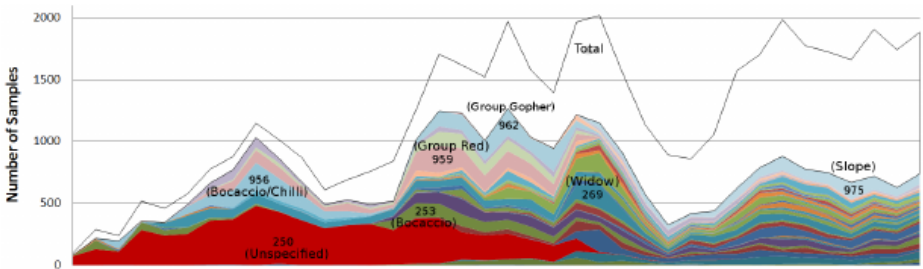
\includegraphics[width=\textwidth]{../pictures/mcatColors.png}
$~$\\
\vspace*{-1cm}
\hspace*{-0.2cm}
\includegraphics[width=1.055\textwidth]{../pictures/stratAvgSamp.pdf}
$~$\\
\vspace*{-2.1cm}
\hspace*{-0.2cm}
\includegraphics[width=1.055\textwidth]{../pictures/nMcatsEMA.pdf}
\end{frame}

%
%

%
\subsection{}
\begin{frame}
\centering
%\vspace{-1.2cm}
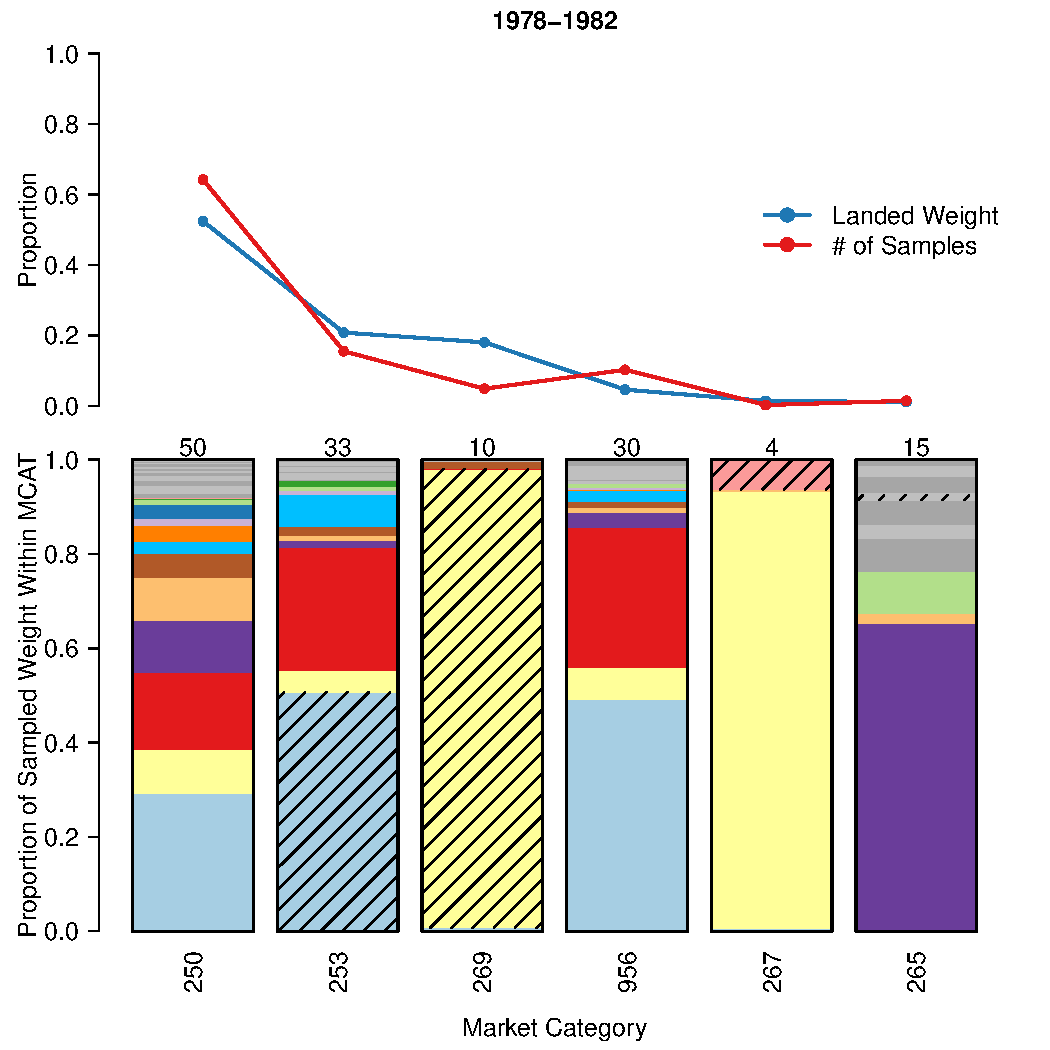
\includegraphics[height=\textheight]{../pictures/1978to1982Bar3.pdf}
%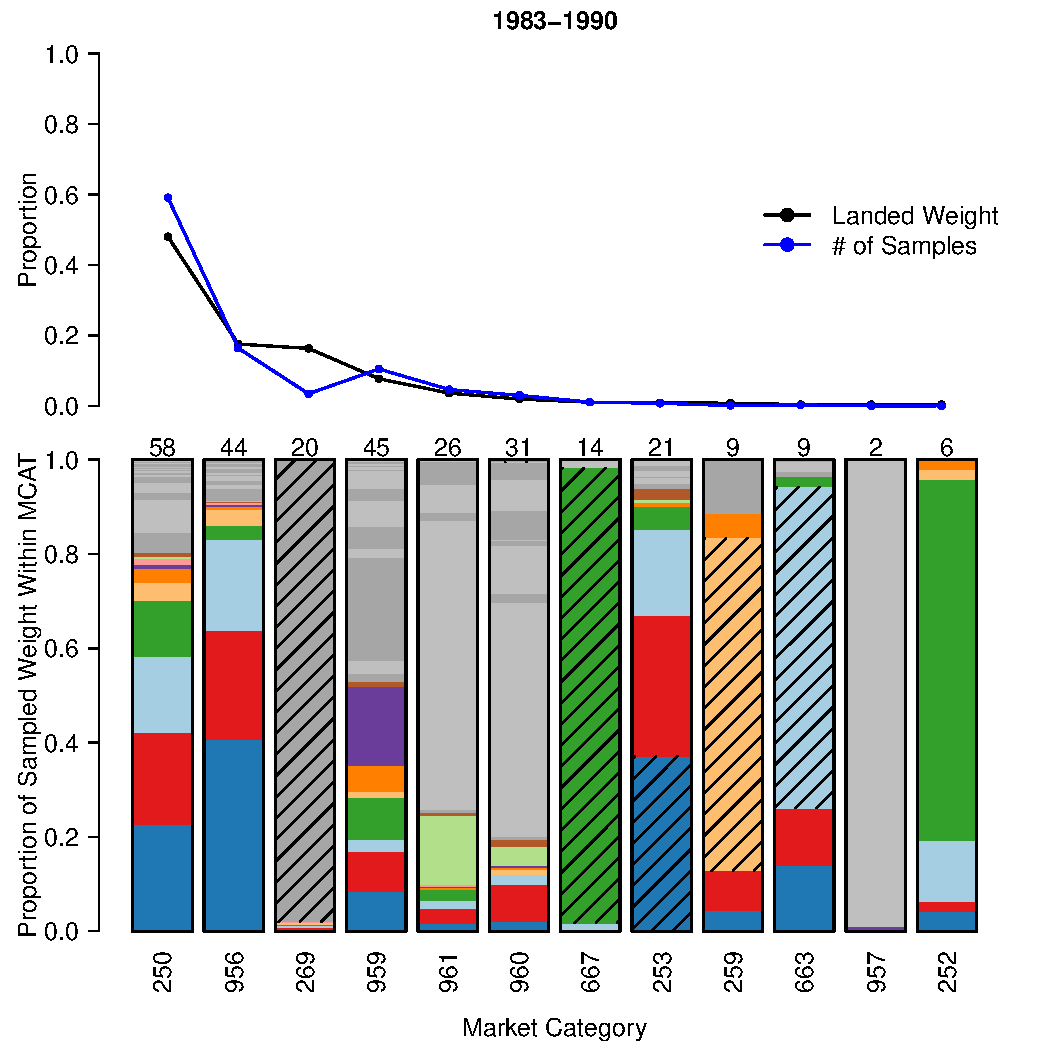
\includegraphics[width=0.43\textwidth]{../pictures/1983to1990Bar3.pdf}
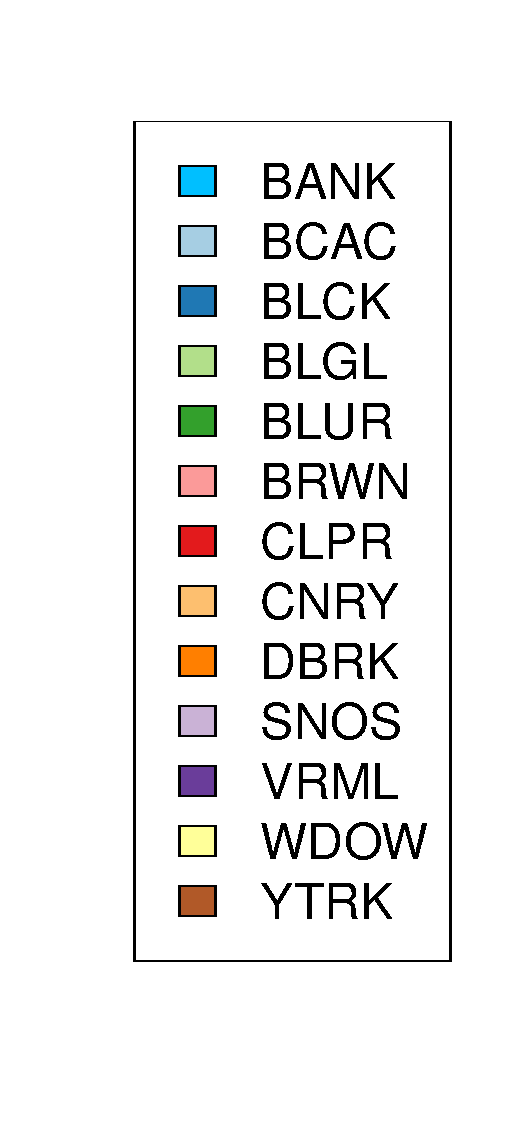
\includegraphics[height=\textheight]{../pictures/barplotLegend.pdf}
\end{frame}

%
%

%
%\subsection{}
\begin{frame}
\centering
%\vspace{-1.2cm}
%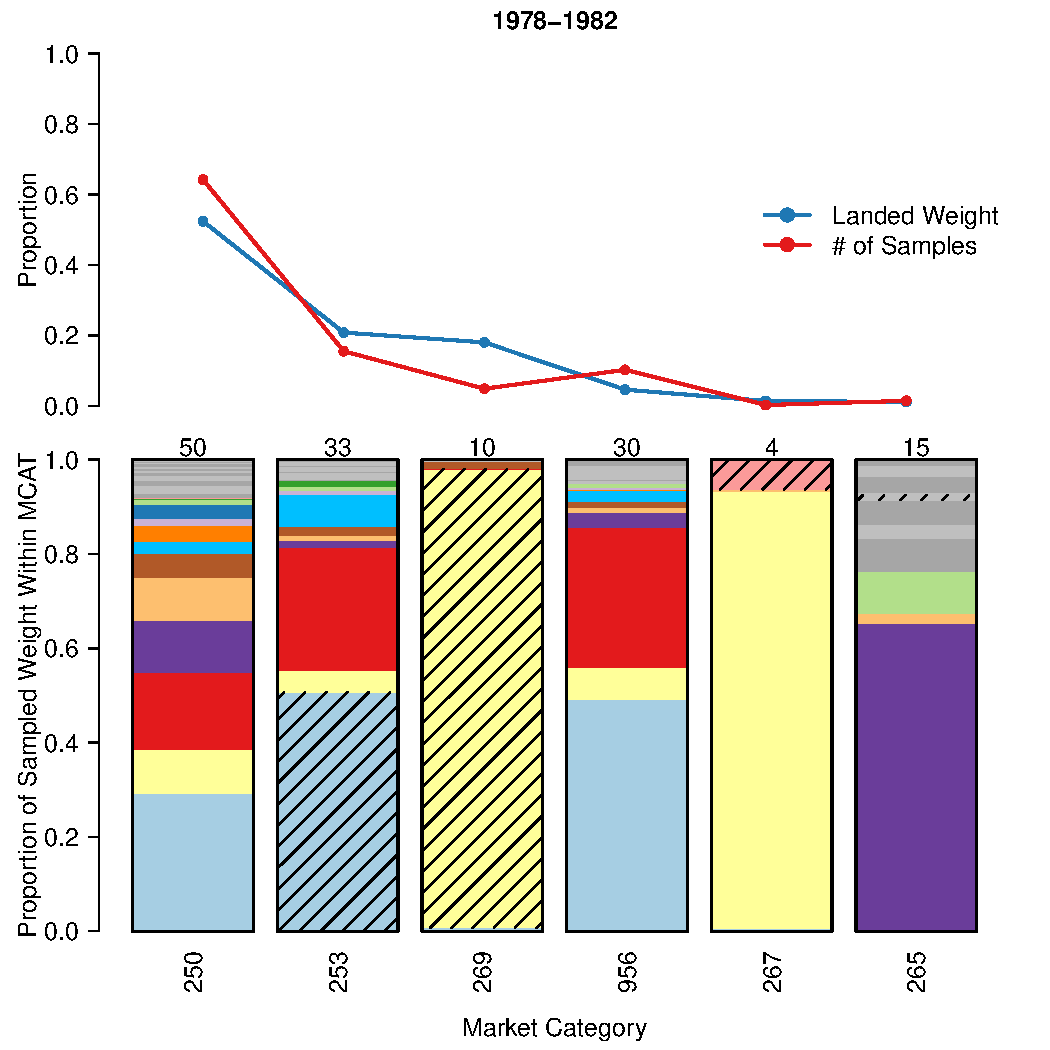
\includegraphics[width=0.43\textwidth]{../pictures/1978to1982Bar3.pdf}
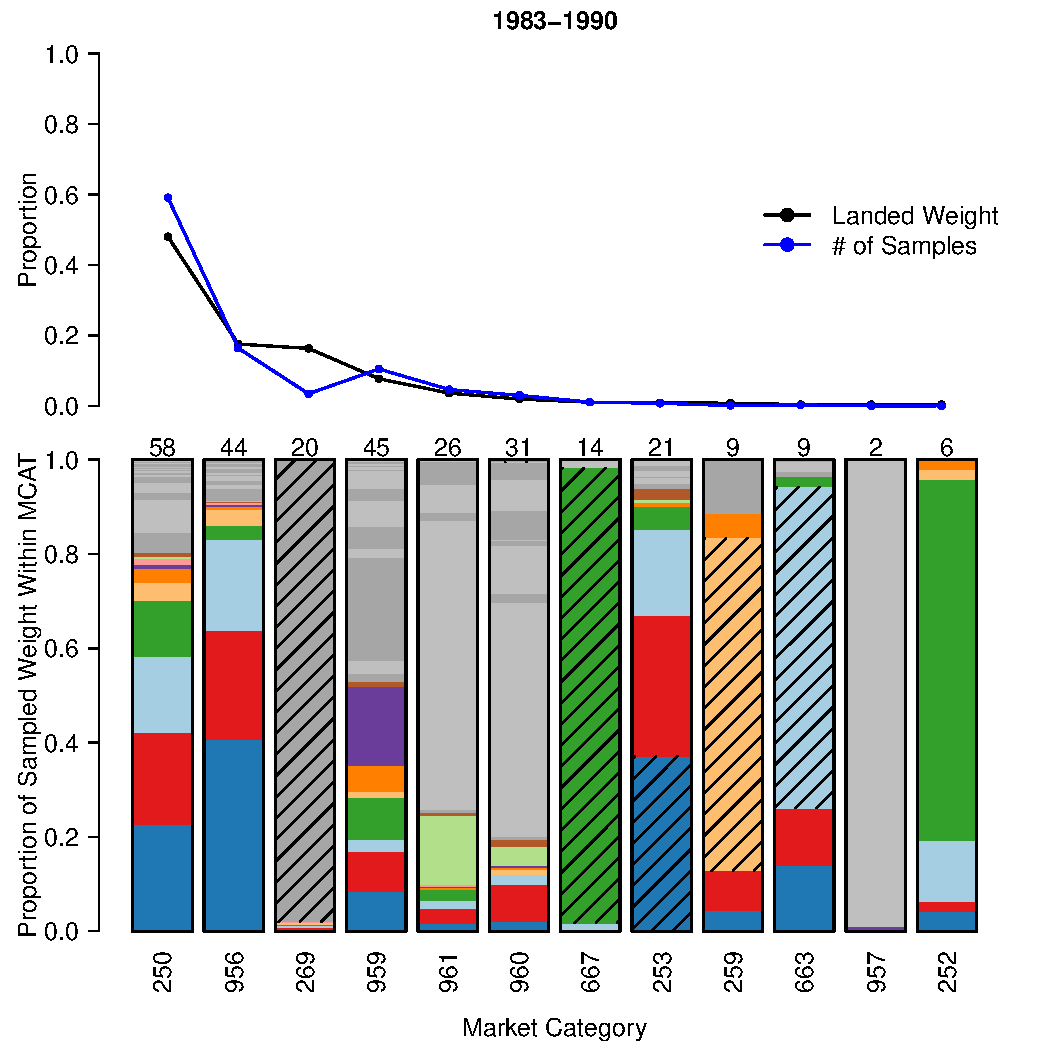
\includegraphics[height=\textheight]{../pictures/1983to1990Bar3.pdf}
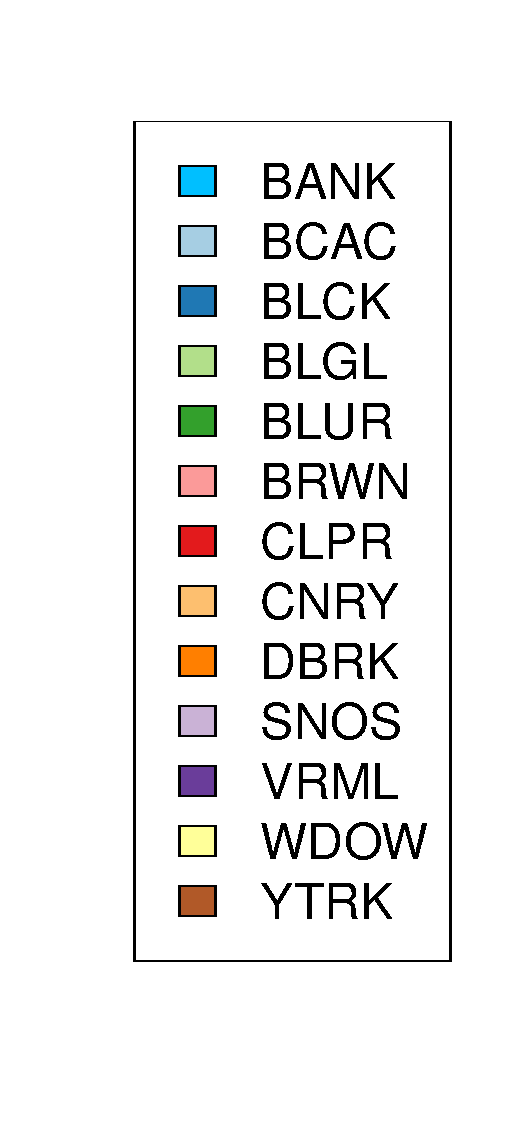
\includegraphics[height=\textheight]{../pictures/barplotLegend.pdf}
\end{frame}

%
%

%
\subsection{}
\begin{frame}
{\color{red}
\begin{itemize}
\item sparce data -> Pooling and heirarchical models
\item integer overdispersion (Motivate next slide)
\end{itemize}
}
\end{frame}

%
%

%
\section{Modeling}
\subsection{}
\begin{frame}{Likelihood}
$y_{ij}$: $i^{\text{th}}$ sample of the $j^{\text{th}}$ species' integer 
weight from market category 250, in the Monterey port complex trawl
fishery for the second quarter of 1982.
% $k^{\text{th}}$ port, caught with the $l^{\text{th}}$ gear, in the $\eta^{\text{th}}$ \mbox{quarter,} of year $m$, for a particular market \mbox{category.}
%$y_{ij}$ is data

%\hspace*{-1cm}
\begin{minipage}{0.24\textwidth}
%\hspace*{-1cm}
\begin{eqnarray*}
y_{ij} \sim \text{Pois}(\theta_j)
%\prod_{ij}\frac{\theta_j^{y_{ij}}e^{-\theta_j}}{y_{ij}!}
\end{eqnarray*}
\end{minipage}
%\hspace*{-0.5cm}
\begin{minipage}{0.24\textwidth}
\begin{eqnarray*}
y_{ij} \sim \text{Bin}(\theta_j)
%\prod_{ij} \left(\substack{n_{ij}\\y_{ij}}\right) \theta_{j}^{y_{ij}} (1-\theta_{j})^{n_{ij}-y_{ij}}&
\end{eqnarray*}
\end{minipage}
%\hspace*{0.5cm}
\begin{minipage}{0.24\textwidth}
\begin{eqnarray*}
y_{ij} \sim \text{NB}(\theta_j, \phi)
\end{eqnarray*}
\end{minipage}
%\hspace*{1cm}
\begin{minipage}{0.24\textwidth}
\begin{eqnarray*}
y_{ij} \sim \text{BB}(\theta_j, \phi)
%\substack{n_{ij}\\y_{ij}}\right)\text{B}()
\end{eqnarray*}
\end{minipage}
\end{frame}

%\subsection{}
\begin{frame}
\hspace*{-1.05cm}
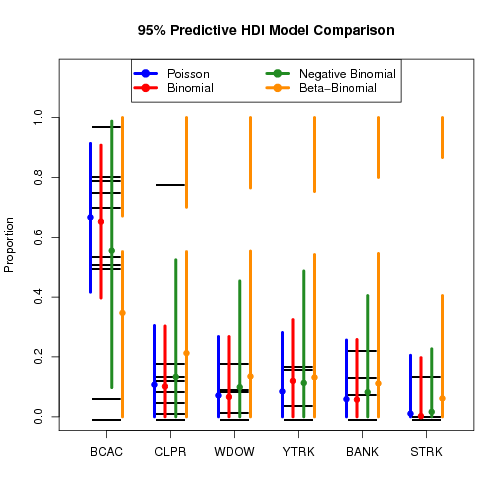
\includegraphics[width=0.6\textwidth]{../pictures/compPlot1982Qtr2.png}
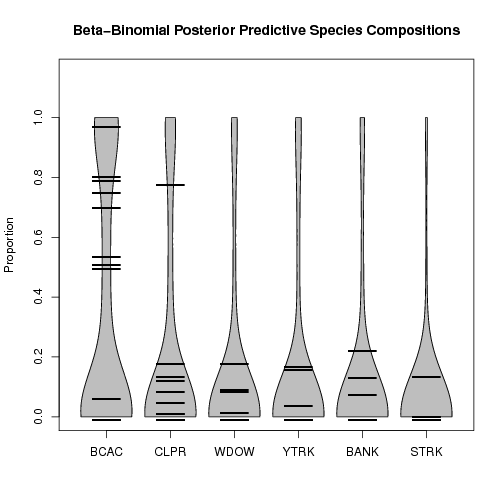
\includegraphics[width=0.6\textwidth]{../pictures/compVioplotQtr2.png}
\end{frame}

%\subsection{}
%\begin{frame}
%\centering
%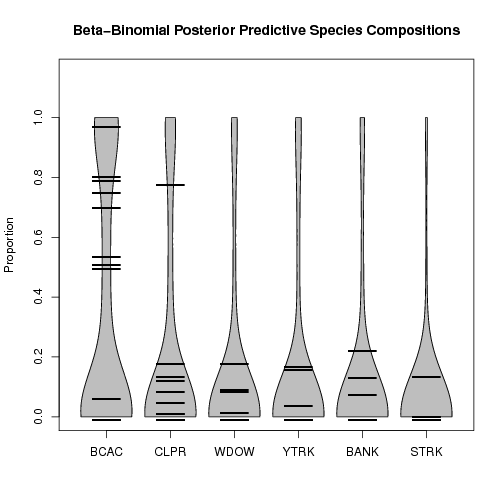
\includegraphics[height=\textheight]{../pictures/compVioplotQtr2.png}
%\end{frame}

%\subsection{}
\begin{frame}
\centering
\resizebox{\textwidth}{!}{\begin{tabular}[c]{@{}lcccc@{}}
%\toprule
\hline
& Poisson & Binomial & NB & BB \\ \hline
%\midrule
%\endhead
MSE & 0.06412 & 0.06264 & 0.05171 & 0.04479 \\
\(\Delta\) DIC & 1001.41 & 1230.60 & 5.03 & 0 \\
\(\Delta\) WAIC & 1079.95 & 1323.75 & 3.43 & 0 \\
\(pr(M|y)\) & \(\approx0\) & \(\approx0\) & \(\approx10^{-7}\) & \(\approx1-10^{-7}\) \\ \hline
%\bottomrule
\end{tabular}}
\end{frame}

%
%

%\section{}
\subsection{}
\begin{frame}{Beta-Binomial Model}
\vspace{-0.5cm}
%\begin{align*}
\begin{equation*}
        y_{ijklm\eta} \sim \text{Beta-Binomial}\Big(\mu_{jklm\eta},~\sigma^2_{jklm\eta} \Big)
\end{equation*}
\vspace{-0.7cm}
\begin{gather*}
%	\vspace{0.2cm}
	\mu_{jklm\eta} = n~\text{logit}^{-1}(\theta_{jklm\eta})\\
	%=n~\frac{\alpha_{jklm\eta}}{\alpha_{jklm\eta}+\beta_{jklm\eta}}  
	\sigma^2_{jklm\eta} = \mu_{jklm\eta}\Big(1-\frac{\mu_{jklm\eta}}{n}\Big)\Big(1+(n-1)~\rho\Big)
	%\sigma^2_{jklm\eta} = \bigg(\mu_{jklm\eta}-\frac{\mu^2_{jklm\eta}}{n}\bigg)\bigg(1+(n-1)~\rho\bigg)
%	\vspace{0.2cm}
\end{gather*}
\vspace{-0.2cm}
\begin{equation*}
        \theta_{jklm\eta} = \beta_0 + \beta^{(s)}_j + \beta^{(p)}_k + \beta^{(g)}_l + \color{blue}{\beta^{(t)}_{m\eta}}%\beta^{(y)}_m + \beta^{(q)}_\eta + \beta^{(y:q)}_{m\eta}   %{\color{blue}a_{jklm\eta}} + {\color{OliveGreen}b_{jklm\eta}} %+ c^*_{jklm\eta}
	%=n~\text{logit}^{-1}(\theta_{jklm\eta})
\end{equation*}
\hspace{-0.5cm}
%0.68
\begin{minipage}[h!]{0.55\textwidth}
	$~$\\
	$y_{ijklm\eta}$: $i^{\text{th}}$ sample of the $j^{\text{th}}$ species' integer weight, in the $k^{\text{th}}$ port, caught with the $l^{\text{th}}$ gear, in the $\eta^{\text{th}}$ \mbox{quarter,} of year $m$, for a particular market \mbox{category.}
\end{minipage}
\begin{minipage}{0.45\textwidth}
	\vspace{-0.5cm}
	\hspace{4cm}
        \begin{eqnarray*}
        j &\in&\left\{1, ..., J\right\} \text{Species}\\
        k &\in&\left\{1, ..., K\right\} \text{Ports}\\
        l &\in&\left\{1, ..., L\right\} \text{Gears}\\
        m &\in&\left\{1, ..., M\right\} \text{Years}\\
        \eta &\in&\left\{1, ..., H\right\} \text{Quarters}
        \end{eqnarray*}
\end{minipage}
\end{frame}

%
%

%
%\subsection{}
\begin{frame}{Time Model}
\hspace*{-0.5cm}
\begin{minipage}{0.3\textwidth}
\begin{center}
\textbf{(M1)}
\begin{eqnarray*}
&\beta^{(t)}_{m\eta} = \beta^{(y)}_{m} + \beta^{(q)}_{\eta}&\\
&\beta^{(y)}_{m} \sim N(0, 32^2)&\\
&\beta^{(q)}_{\eta} \sim N(0, 32^2)&\\
&~&
\end{eqnarray*}
\end{center}

\begin{center}
\textbf{(M4)}
\begin{eqnarray*}
&\beta^{(t)}_{m\eta} = \beta^{(y:q)}_{m\eta}&\\
&\beta^{(y:q)}_{m\eta} \sim N(0, v)&\\
&~&
\end{eqnarray*}
\end{center}
\end{minipage}
\begin{minipage}{0.3\textwidth}
\begin{center}
\textbf{(M2)}
\begin{eqnarray*}
&\beta^{(t)}_{m\eta} = \beta^{(y)}_{m} + \beta^{(q)}_{\eta}&\\
&\beta^{(y)}_{m} \sim N(0, v^{(y)})&\\
&\beta^{(q)}_{\eta} \sim N(0, v^{(q)})&\\
&~&
\end{eqnarray*}
\end{center}

\begin{center}
\textbf{(M5)}
\begin{eqnarray*}
&\beta^{(t)}_{m\eta} = \beta^{(y:q)}_{m\eta}&\\
&\beta^{(y:q)}_{m\eta} \sim N(0, v_\eta)&\\
&~&
\end{eqnarray*}
\end{center}
\end{minipage}
\begin{minipage}{0.3\textwidth}
\begin{center}
~~~~~~~~~~~~~\textbf{(M3)}
\begin{eqnarray*}
&\beta^{(t)}_{m\eta} = \beta^{(y)}_{m} + \beta^{(q)}_{\eta} + \beta^{(y:q)}_{m\eta} & \\
&\beta^{(y)}_{m} \sim N(0, v^{(y)}) & \\
&\beta^{(q)}_{\eta} \sim N(0, v^{(q)}) & \\
&\beta^{(y:q)}_{m\eta} \sim N(0, v) &
\end{eqnarray*}
\end{center}

\begin{center}
\textbf{(M6)}
\begin{eqnarray*}
&\beta^{(t)}_{m\eta} = \beta^{(y:q)}_{m\eta}&\\
&\beta^{(y:q)}_{m\eta} \sim N(0, v_m)&
\end{eqnarray*}i
\end{center}
\end{minipage}
\end{frame}

%
%

%\subsection{}
\begin{frame}{Priors}
$~$
\hspace{-0.8cm}
\begin{minipage}{0.55\textwidth}
%\vspace{-0.5cm}
\begin{align*}
\beta_0 &\propto 1\\
\beta^{(s)}_j &\sim N(0, 32^2)\\
\beta^{(p)}_k &\sim N(0, 32^2)\\
\beta^{(g)}_l &\sim N(0, 32^2)\\
&\\
\text{logit}(\rho) &\sim N(0, 2^2)\\
&\\
v\sim IG(1,~&2x10^{3}) ~~~\forall~~~v 
\end{align*}
\end{minipage}
\begin{minipage}{0.4\textwidth}       
\includegraphics[width=1.4\textwidth]{../pictures/priorPredict.pdf}
\end{minipage}
\end{frame}

%
%

%\subsection{}
\begin{frame}
\begin{center}
\textbf{1978-1982}
\hspace*{-0.4cm}
\begin{tabular}[c]{@{}lcccccc@{}}
%\toprule
\hline
& M1 & M2 & M3 & M4 & M5 & M6 \\ \hline
%\midrule
%\endhead
MSE & 0.12725 & 0.12704 & 0.12680 & 0.12237 & 0.12724 & 0.12657 \\ %\hline
\(\Delta\) DIC & 2558.56 & 2259.94 & 2013.21 & 0 & 2175.32 & 2174.71 \\ %\hline
\(\Delta\) WAIC & 2562.65 & 2263.58 & 2009.32 & 0 & 2171.18 & 2170.56 \\ %\hline
\(pr(M|y)\) & \(\approx0\) & \(\approx0\) & \(\approx0\) & \(\approx1\) & \(\approx0\) & \(\approx0\) \\ \hline
%\bottomrule
\end{tabular}

$~$\\
\color{red}{
\textbf{1983-1990*}
\hspace*{-0.4cm}
\begin{tabular}[c]{@{}lcccccc@{}}
%\toprule
\hline
& M1 & M2 & M3 & M4 & M5 & M6 \\ \hline
%\midrule
%\endhead
MSE & 0.12724 & 0.12704 & 0.12680 & 0.12237 & 0.12723 & 0.12657 \\ %\hline
\(\Delta\) DIC & 2558.56 & 2259.94 & 2013.21 & 0 & 2175.32 & 2174.71 \\ %\hline
\(\Delta\) WAIC & 2562.65 & 2263.58 & 2009.32 & 0 & 2171.18 & 2170.56 \\ %\hline
\(pr(M|y)\) & \(\approx0\) & \(\approx0\) & \(\approx0\) & \(\approx1\) & \(\approx0\) & \(\approx0\) \\ \hline
%\bottomrule
\end{tabular}
}
\end{center}
\end{frame}

%
%

%
\section{Prediction}
\subsection{}
\begin{frame}{Posterior Predictive Weight Distibutions}
\vspace{-0.5cm}
\begin{equation*}
\hspace{-0.8cm}
p(y^*_{jklm\eta}|\bm{y}) = \int\!\!\!\!\int\! \text{BB}\Big( y^*_{jklm\eta}|\mu_{jklm\eta}, \sigma^2_{jklm\eta} \Big) P\Big(\mu_{jklm\eta}, \sigma^2_{jklm\eta} | \bm{y}\Big) d\mu_{jklm\eta} d\sigma^2_{jklm\eta}
\end{equation*}

\color{red}{motivate prediction for filling holes/hindcasting}\\
\color{red}{show a 100 pound BCAC distribution}

\end{frame}

%
%

%\subsection{}
\begin{frame}
\begin{equation*}
\pi^*_{jklm\eta} = \frac{y^*_{jklm\eta}}{\sum_j y^*_{jklm\eta}} ~~~ \bm{y}^*_{klm\eta}\neq \bm{0}
\end{equation*}
\color{red}{show sppComp distribution for some strata}
%%\vspace{-0.3cm}
%\hspace*{-0.8cm}
%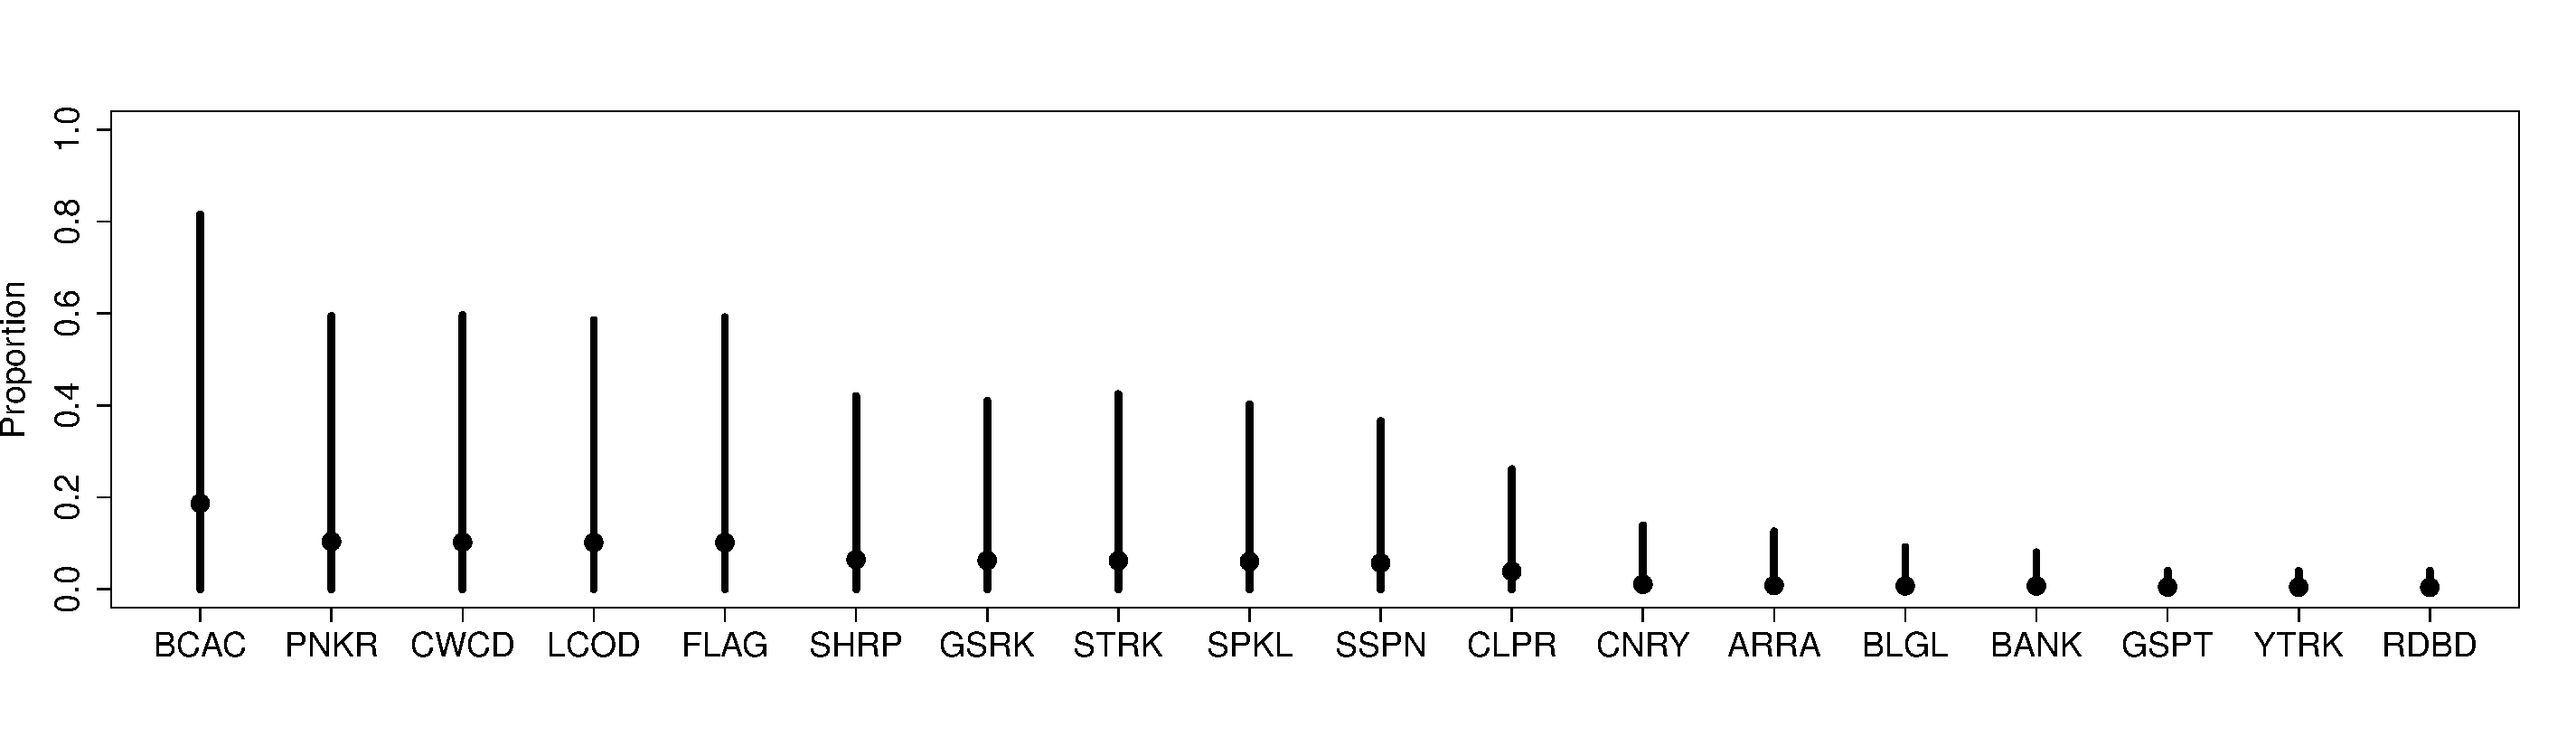
\includegraphics[width=1.15\textwidth]{bocBox1.pdf}
\end{frame}

%
%

\begin{frame}{}
\color{red} Expansion
\end{frame}

%
%

\section{BMA}
\subsection{}
\begin{frame}
\color{red} instructive example of port pooling w/ Bell number and constraints
\end{frame}

%\subsection{}
\begin{frame}{}%{\color{red}ITH} Southern California\color{red}Model Selection Example (Weights, WAIC) $\rightarrow$ look for point conception}
$~$\\
%\vspace{-0.5cm}
\hspace*{-1cm}
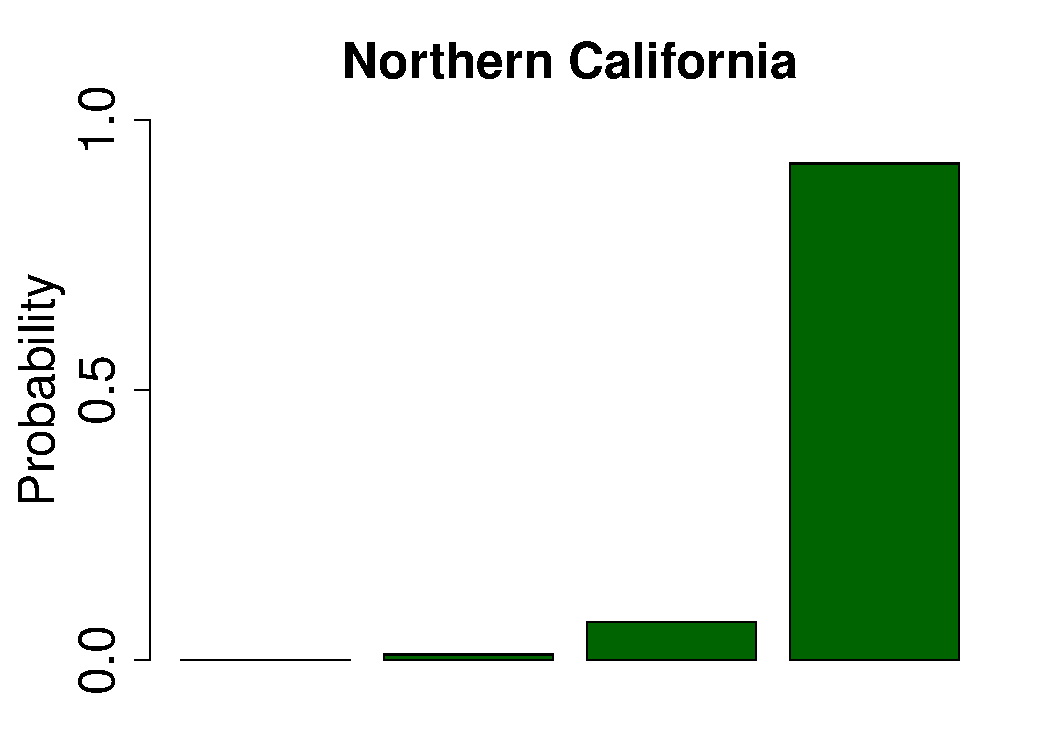
\includegraphics[width=0.6\textwidth]{northern269.pdf}
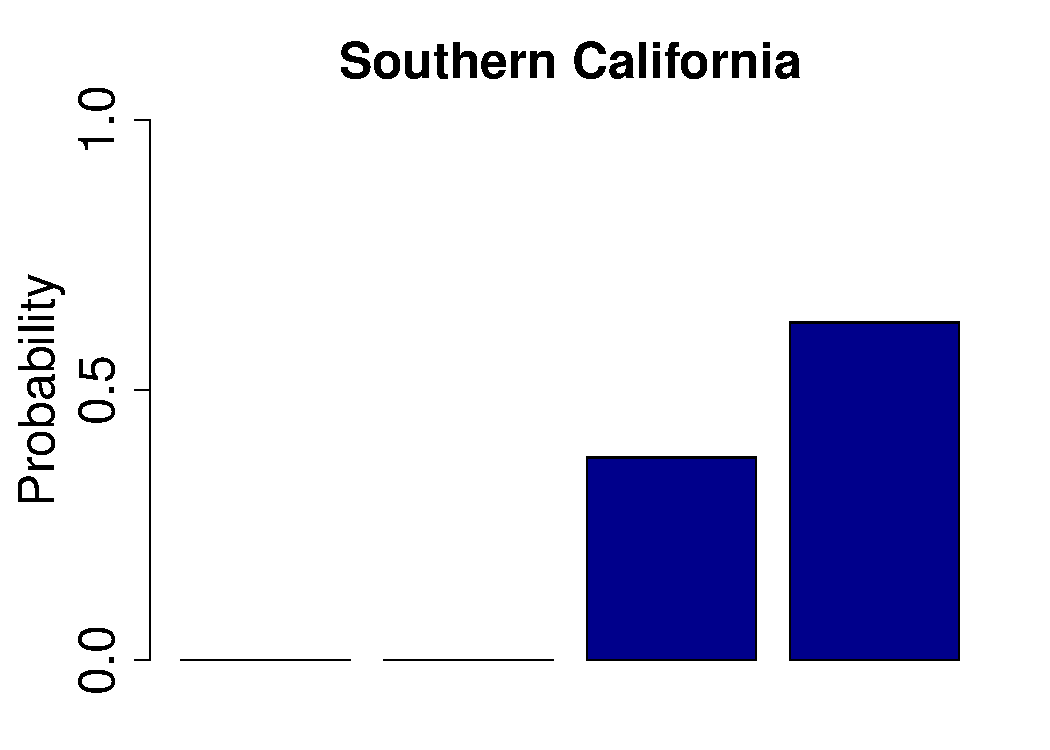
\includegraphics[width=0.6\textwidth]{southern269.pdf}\\
\vspace{-0.5cm}
\hspace*{-0.3cm}
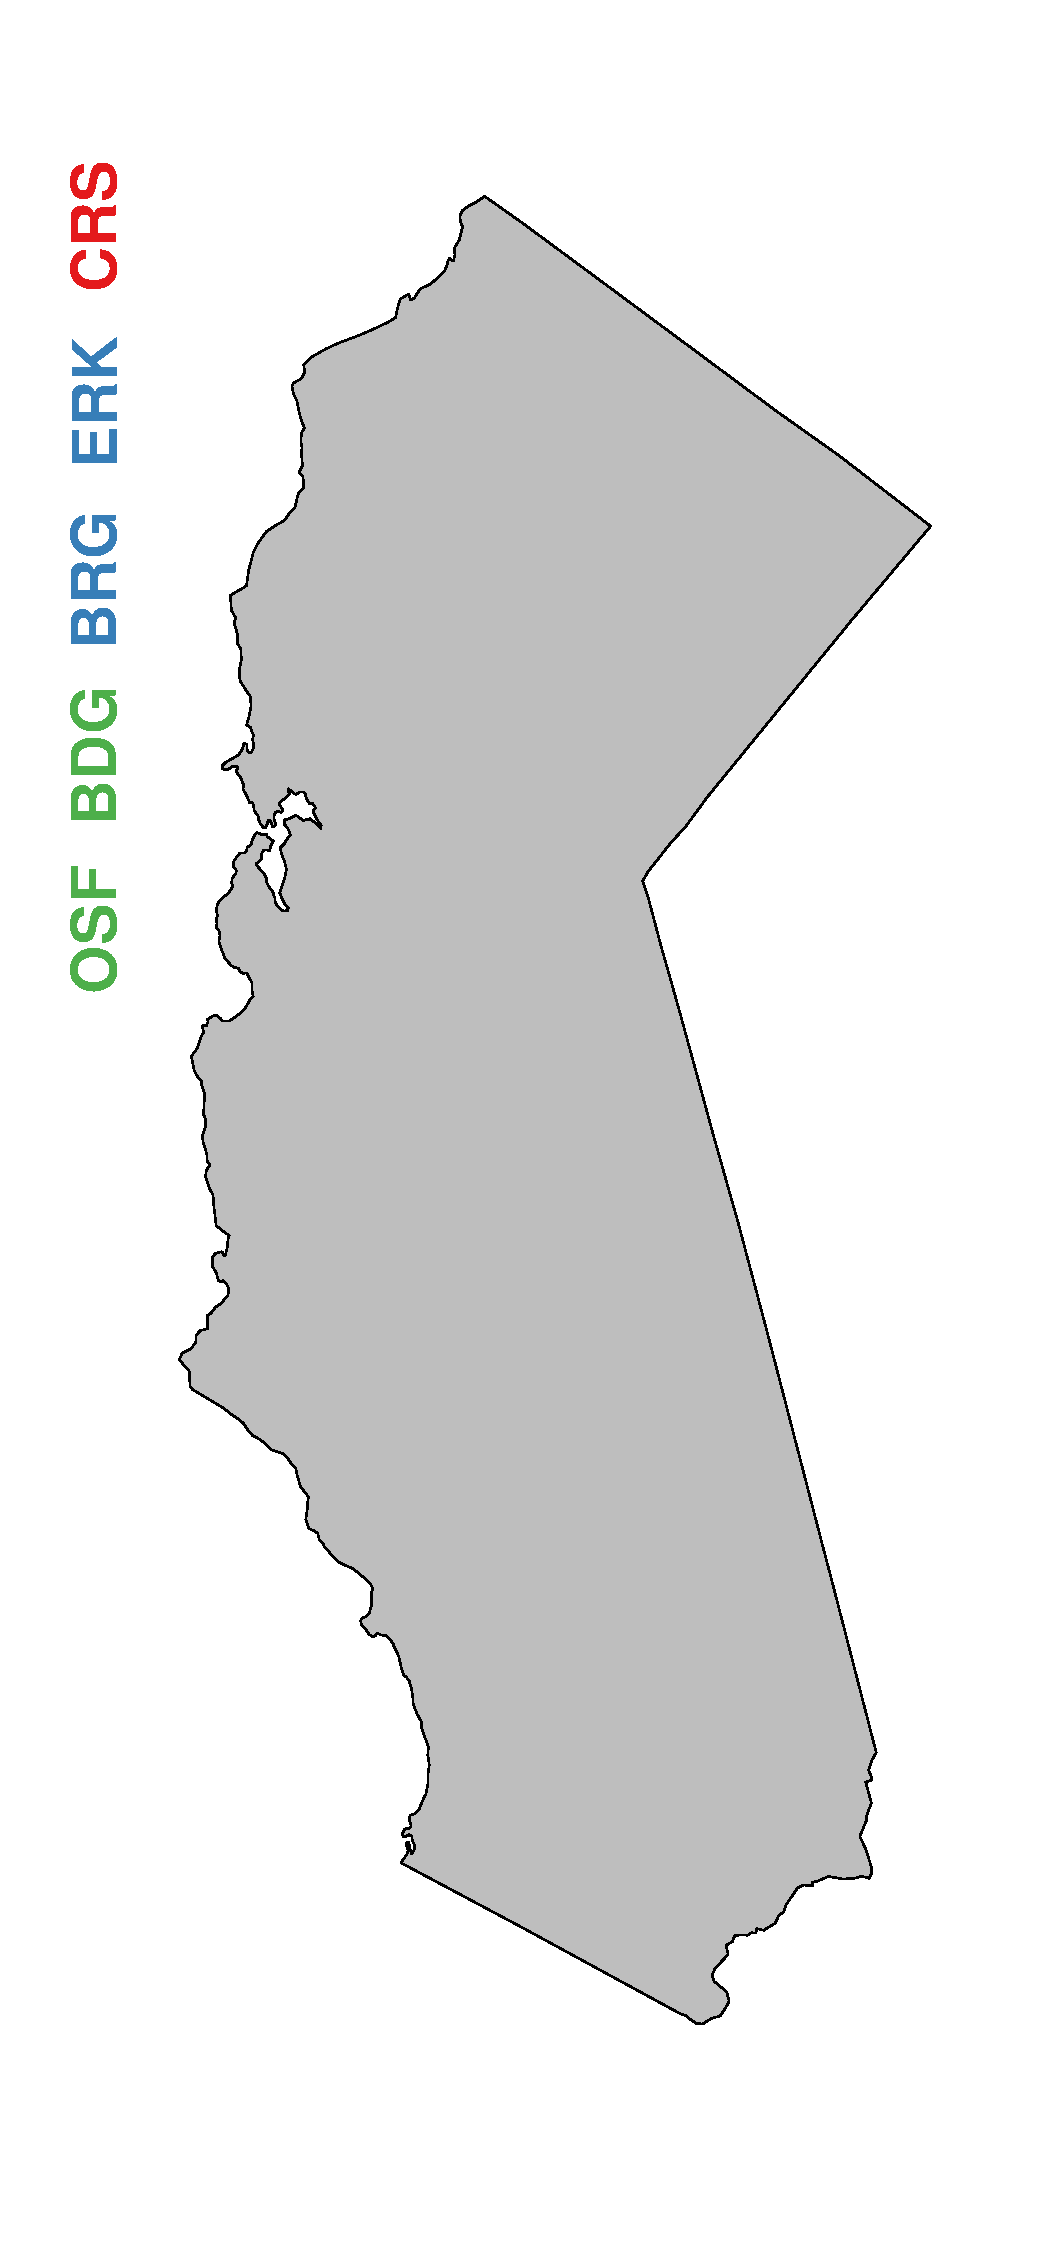
\includegraphics[height=0.37\textheight]{./space10MapTop.pdf}
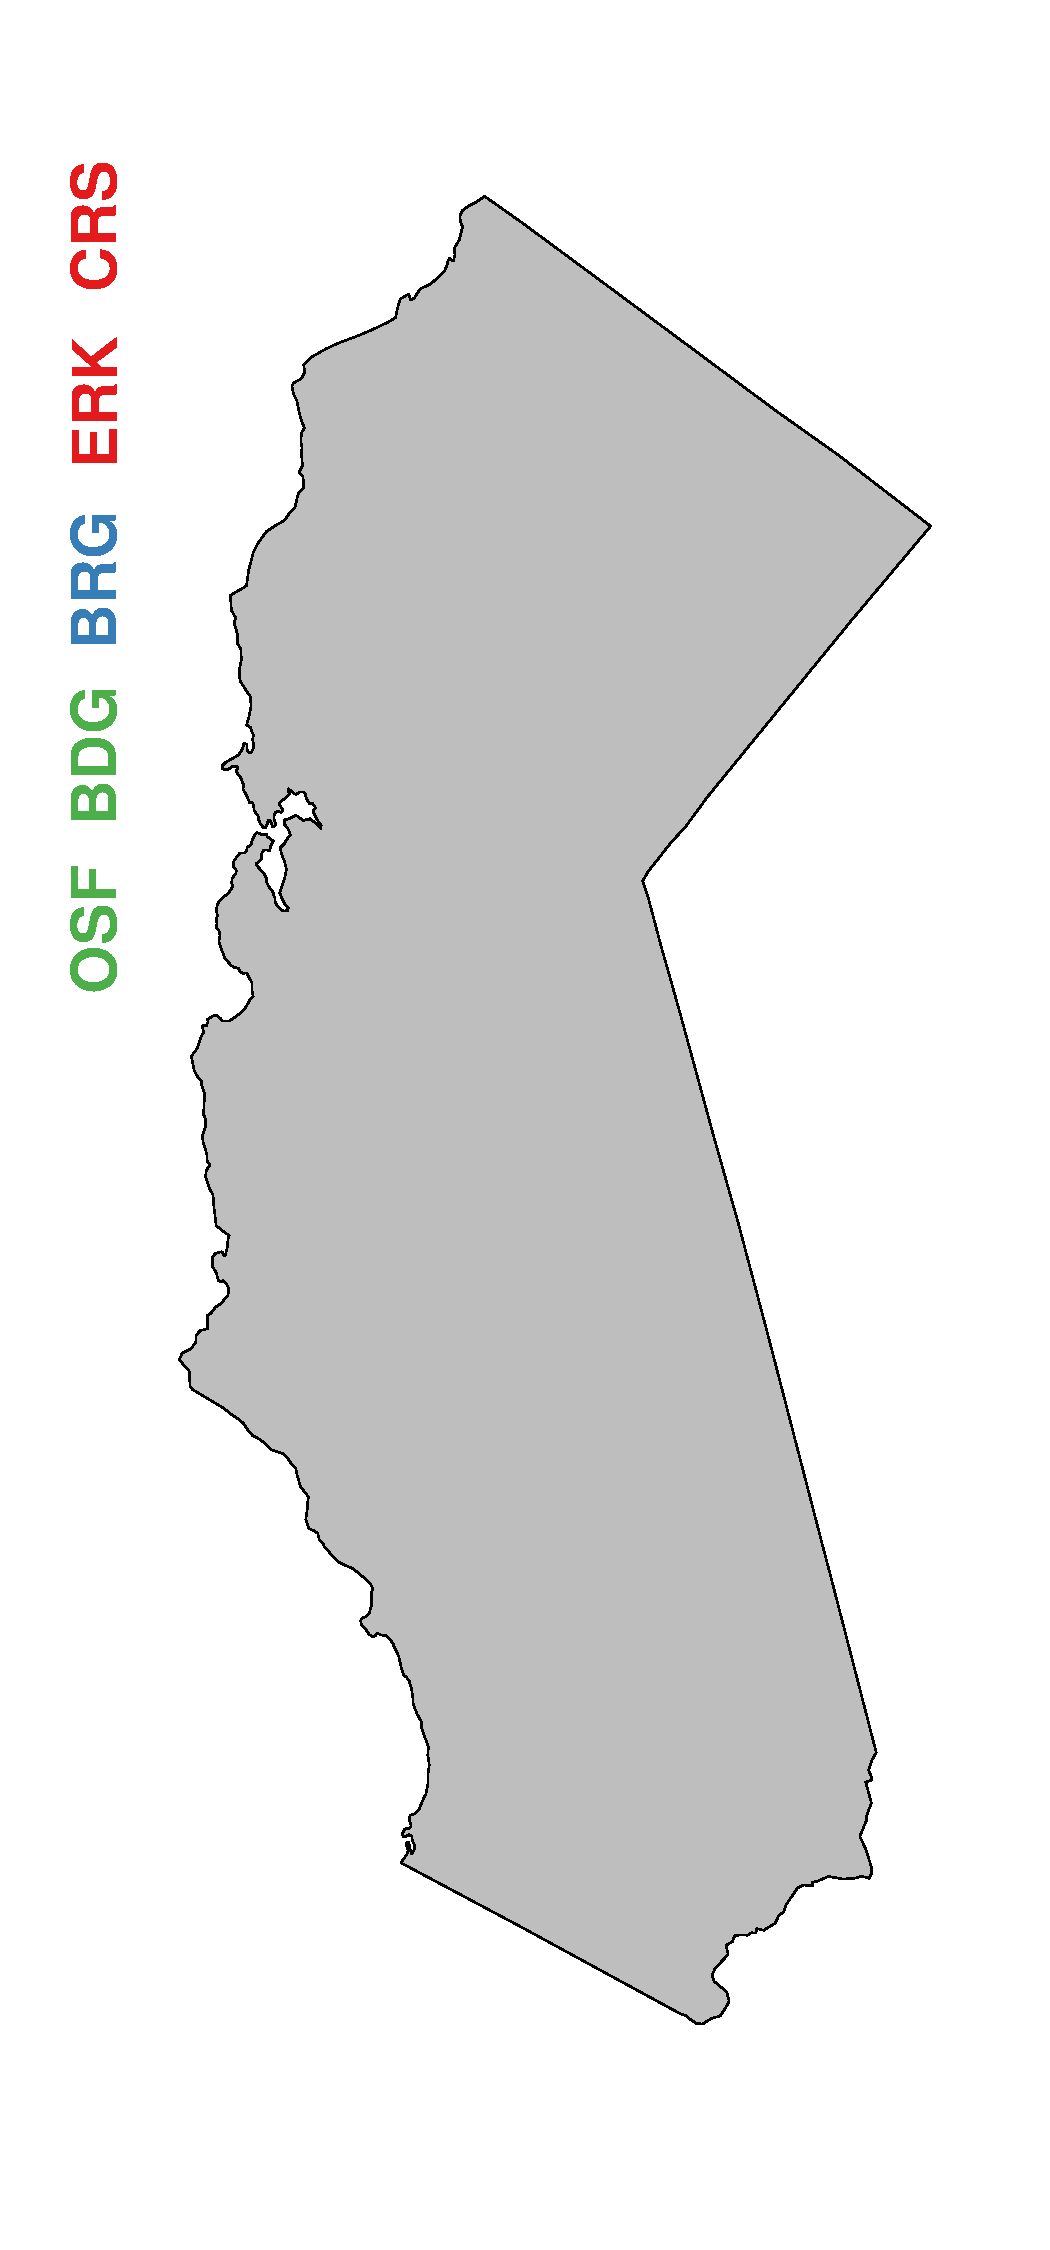
\includegraphics[height=0.37\textheight]{./space9MapTop.pdf}
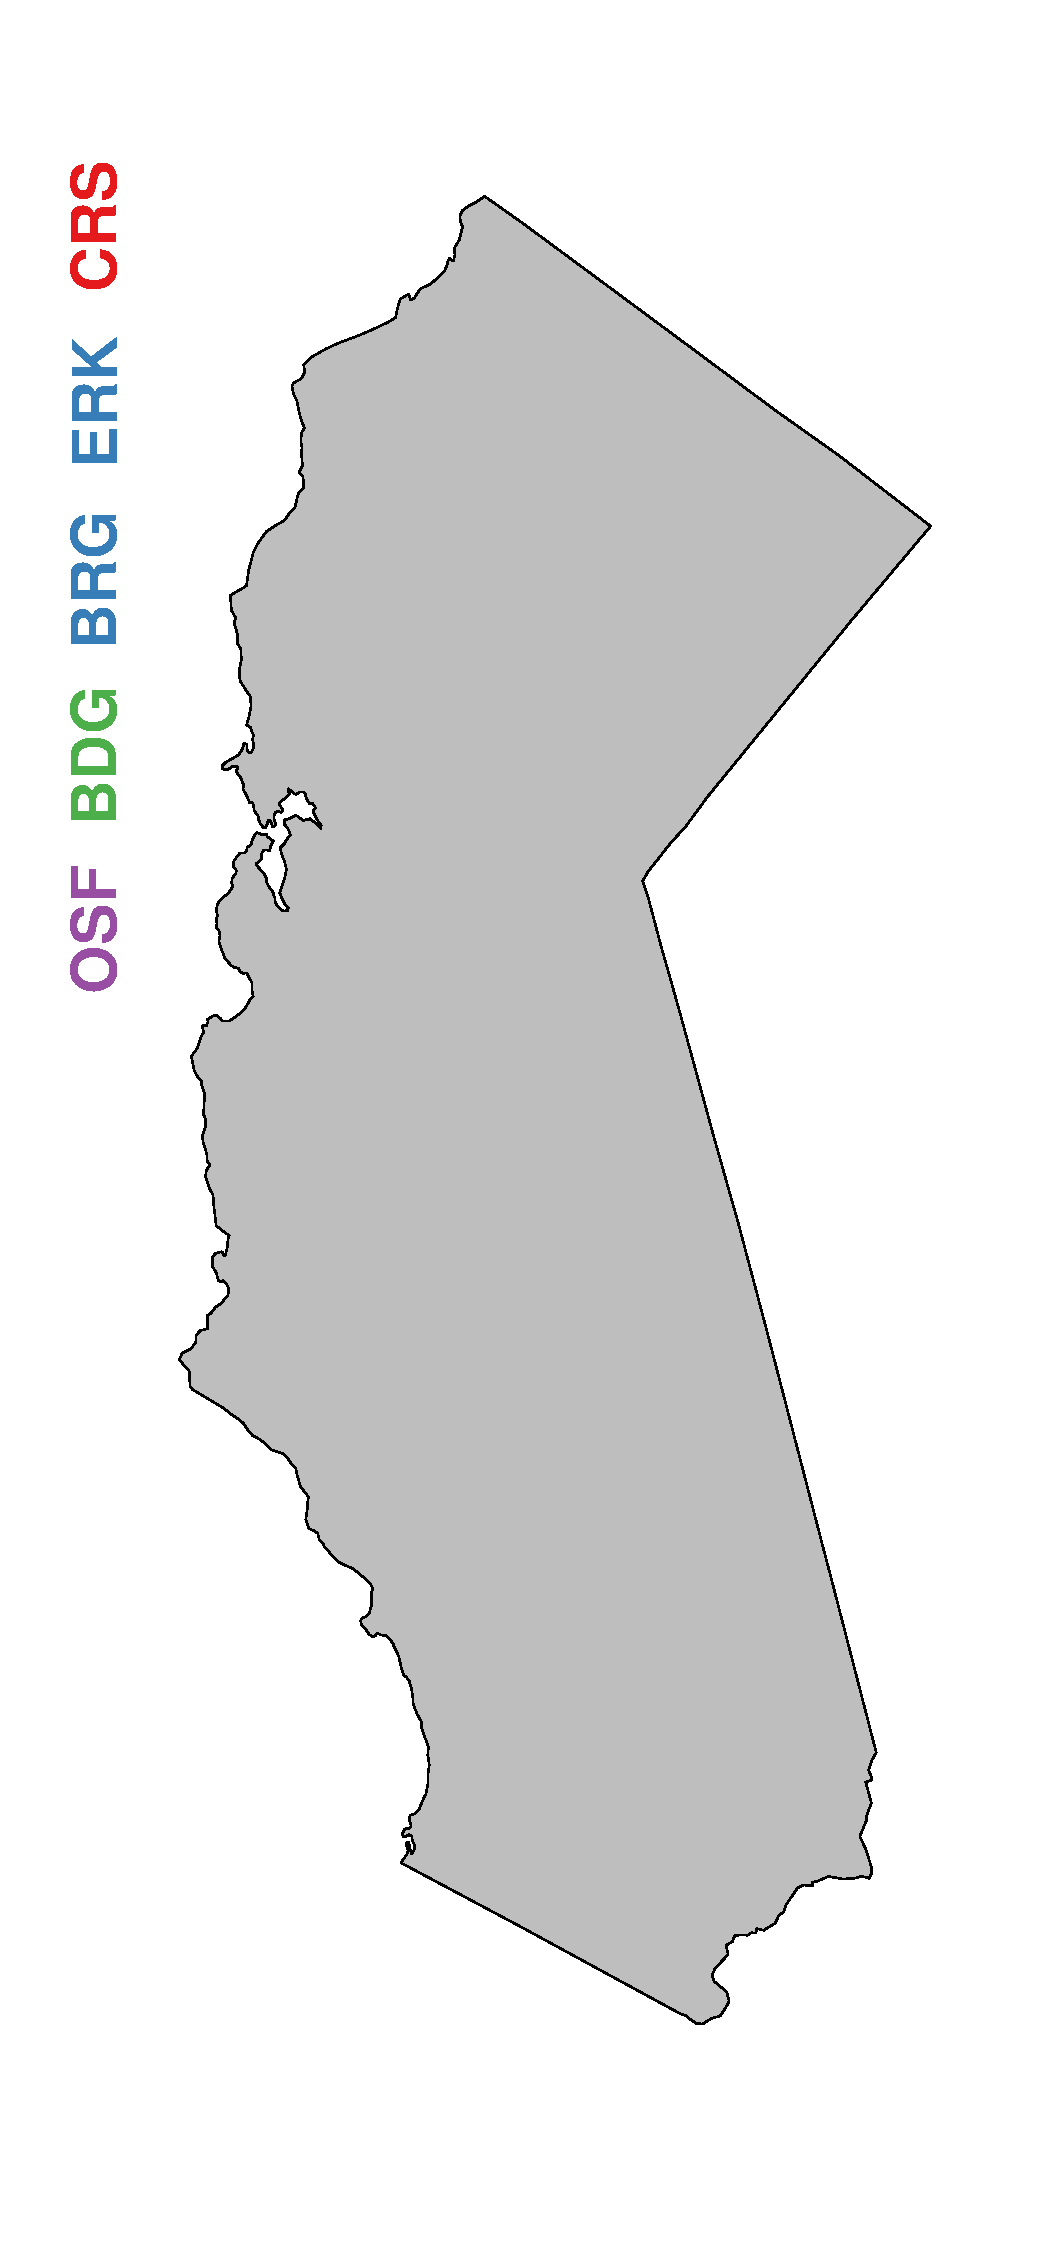
\includegraphics[height=0.37\textheight]{./space14MapTop.pdf}
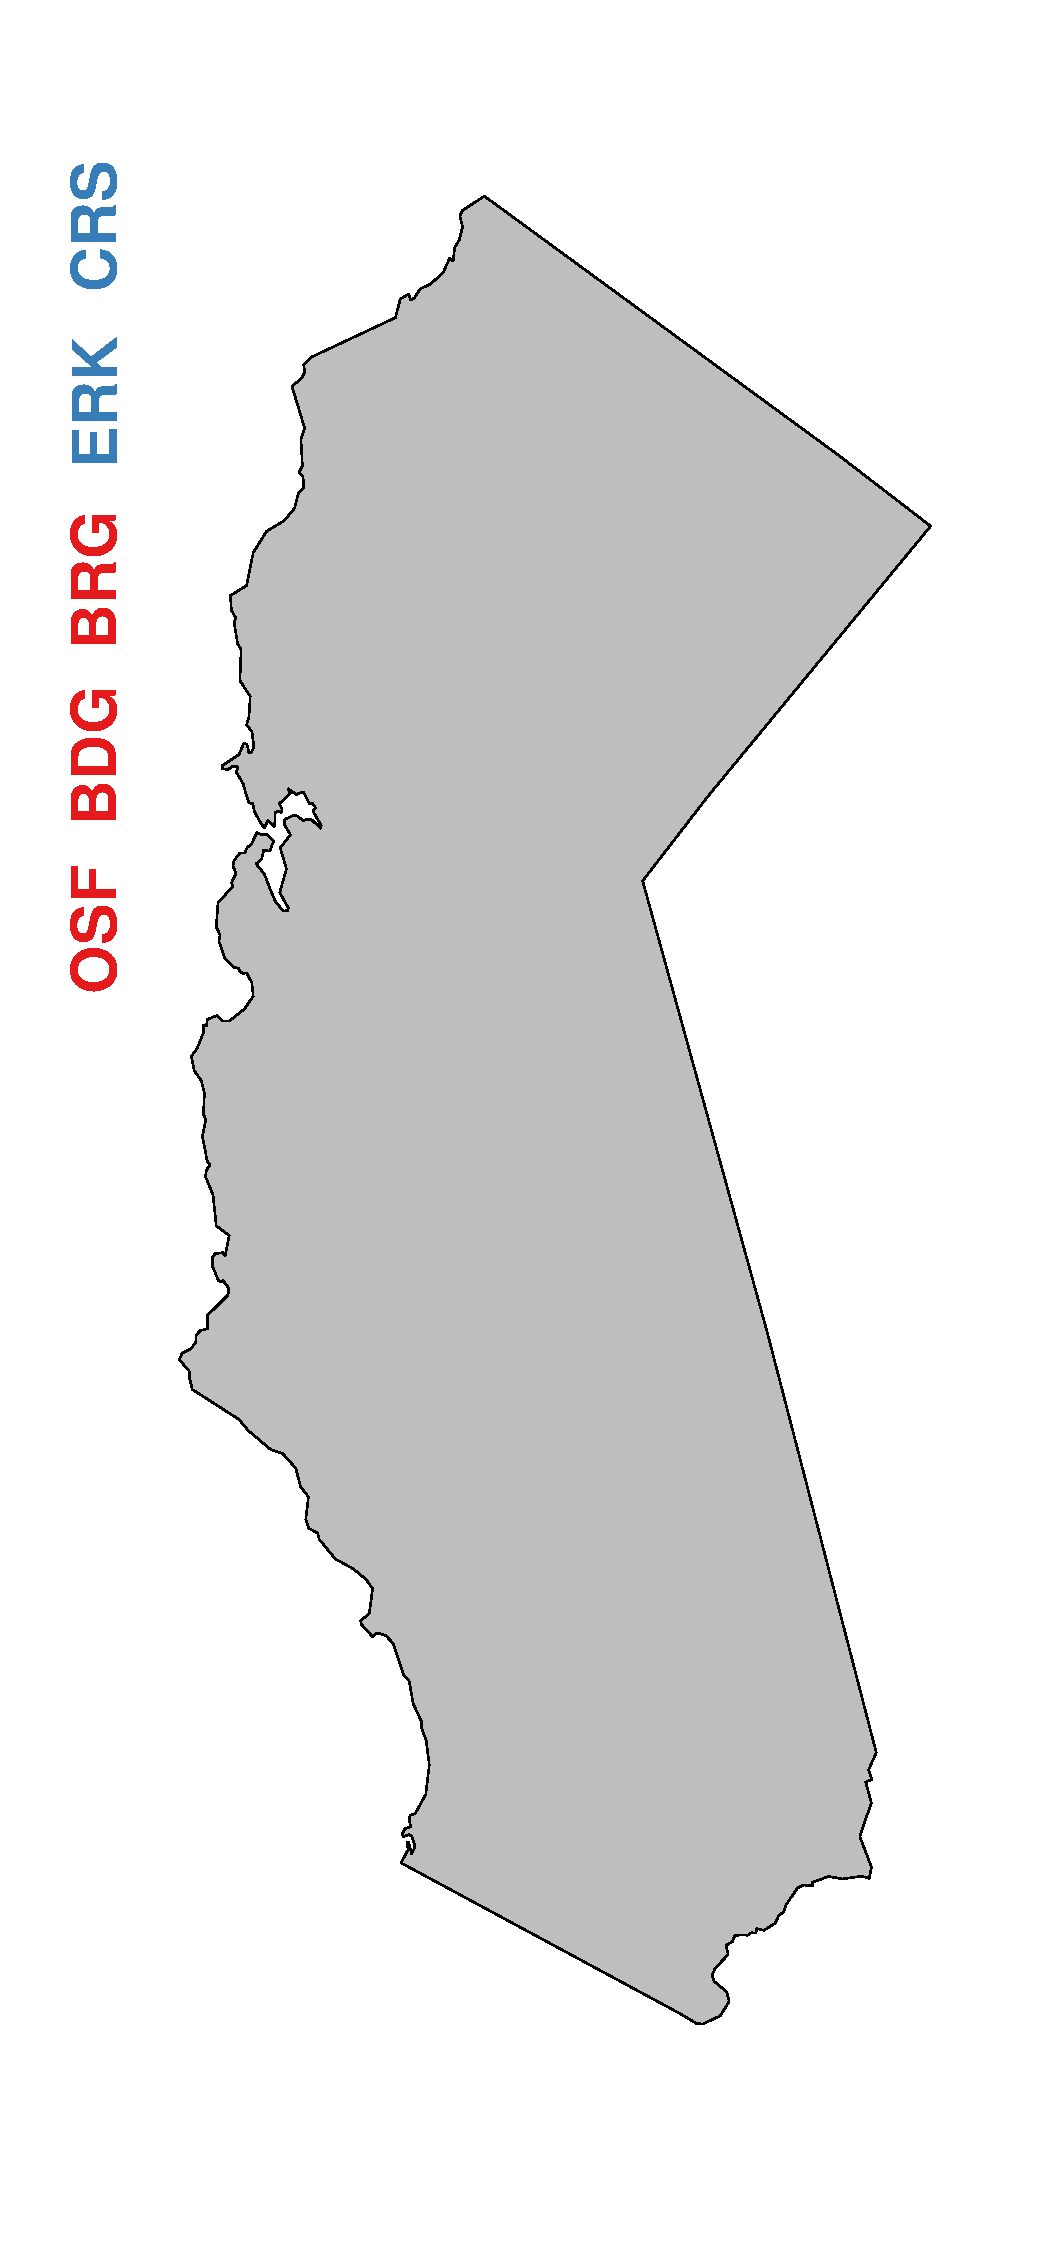
\includegraphics[height=0.37\textheight]{./space4MapTop.pdf}
\hspace*{0.9cm}
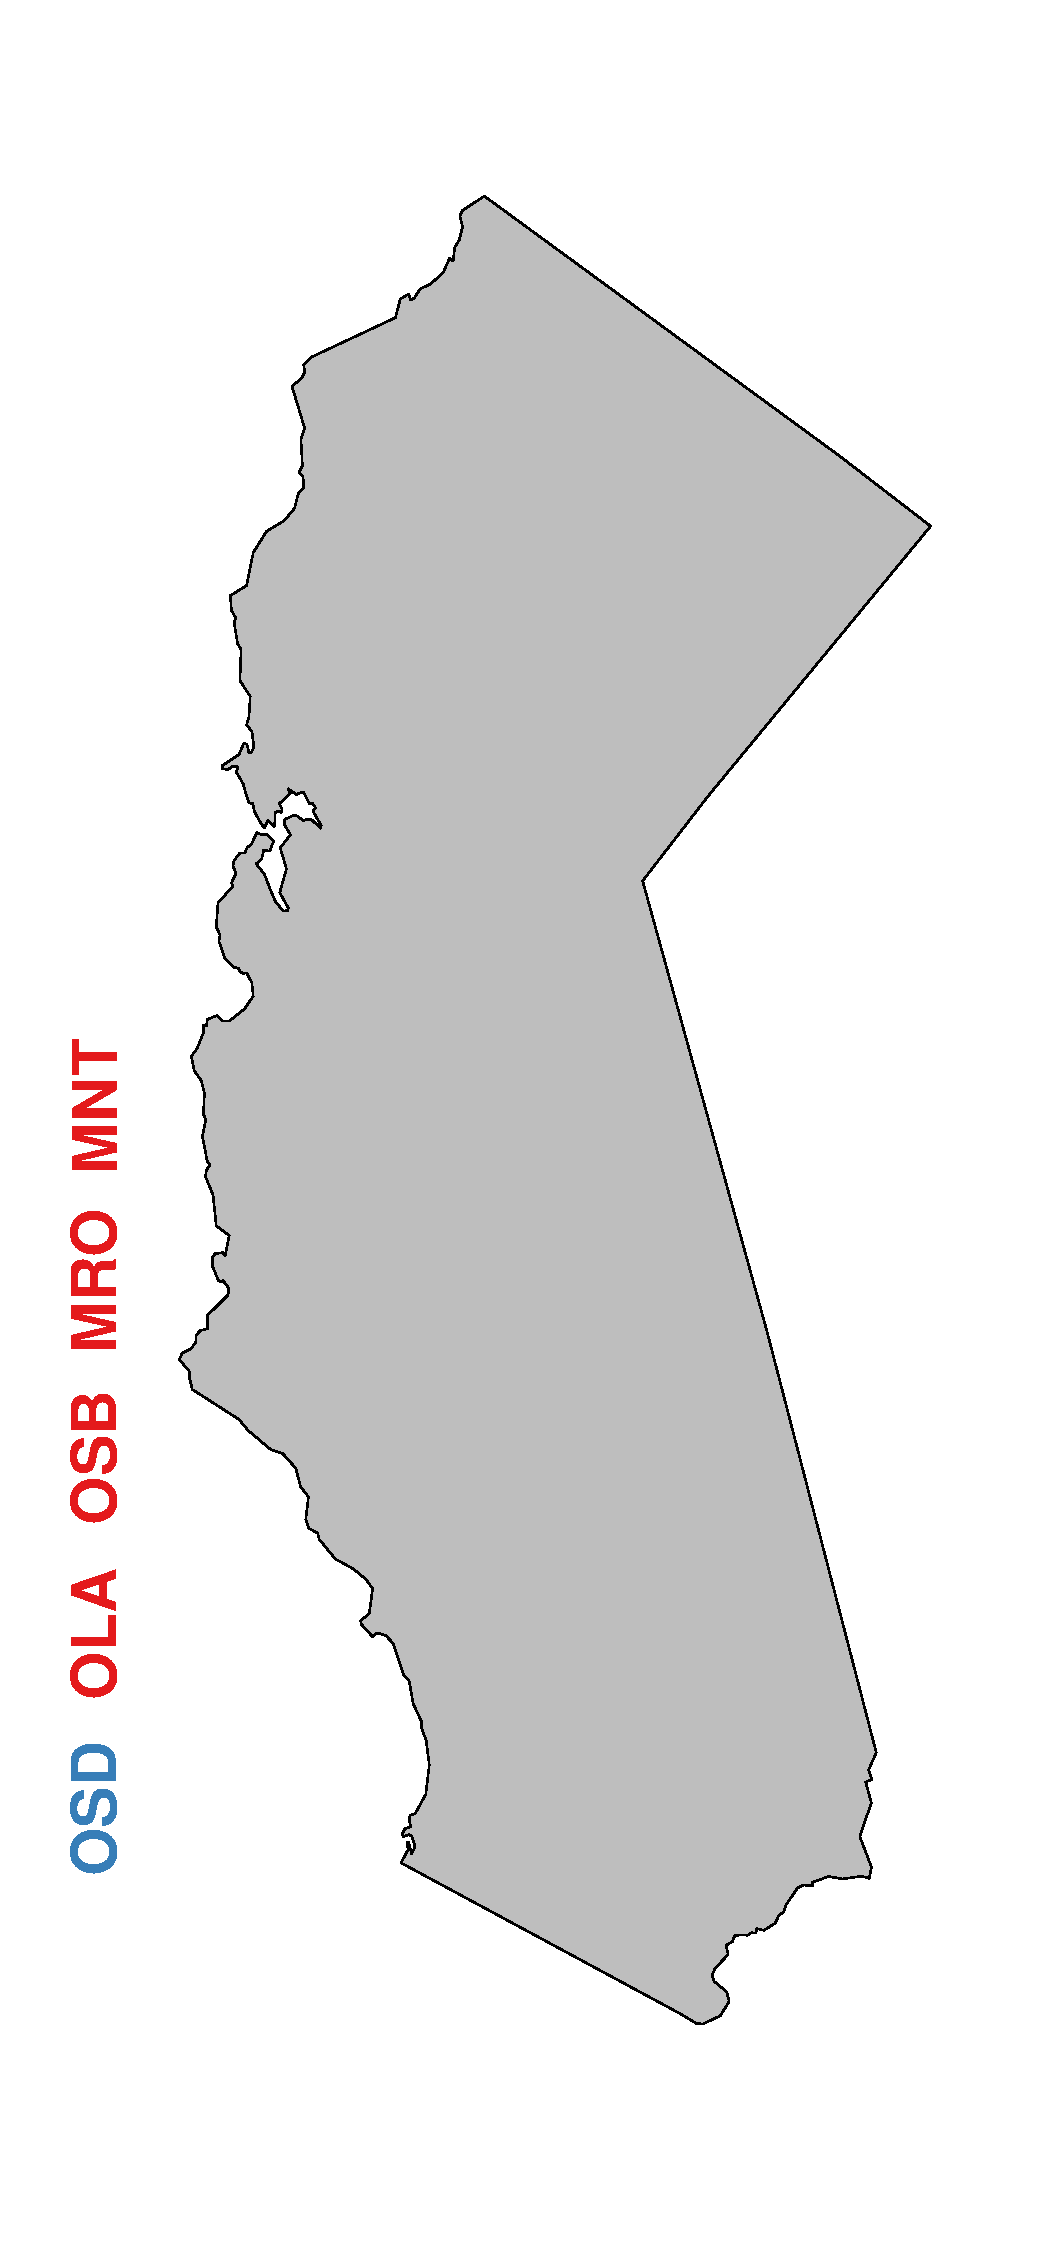
\includegraphics[height=0.37\textheight]{./space2MapBottom.pdf}
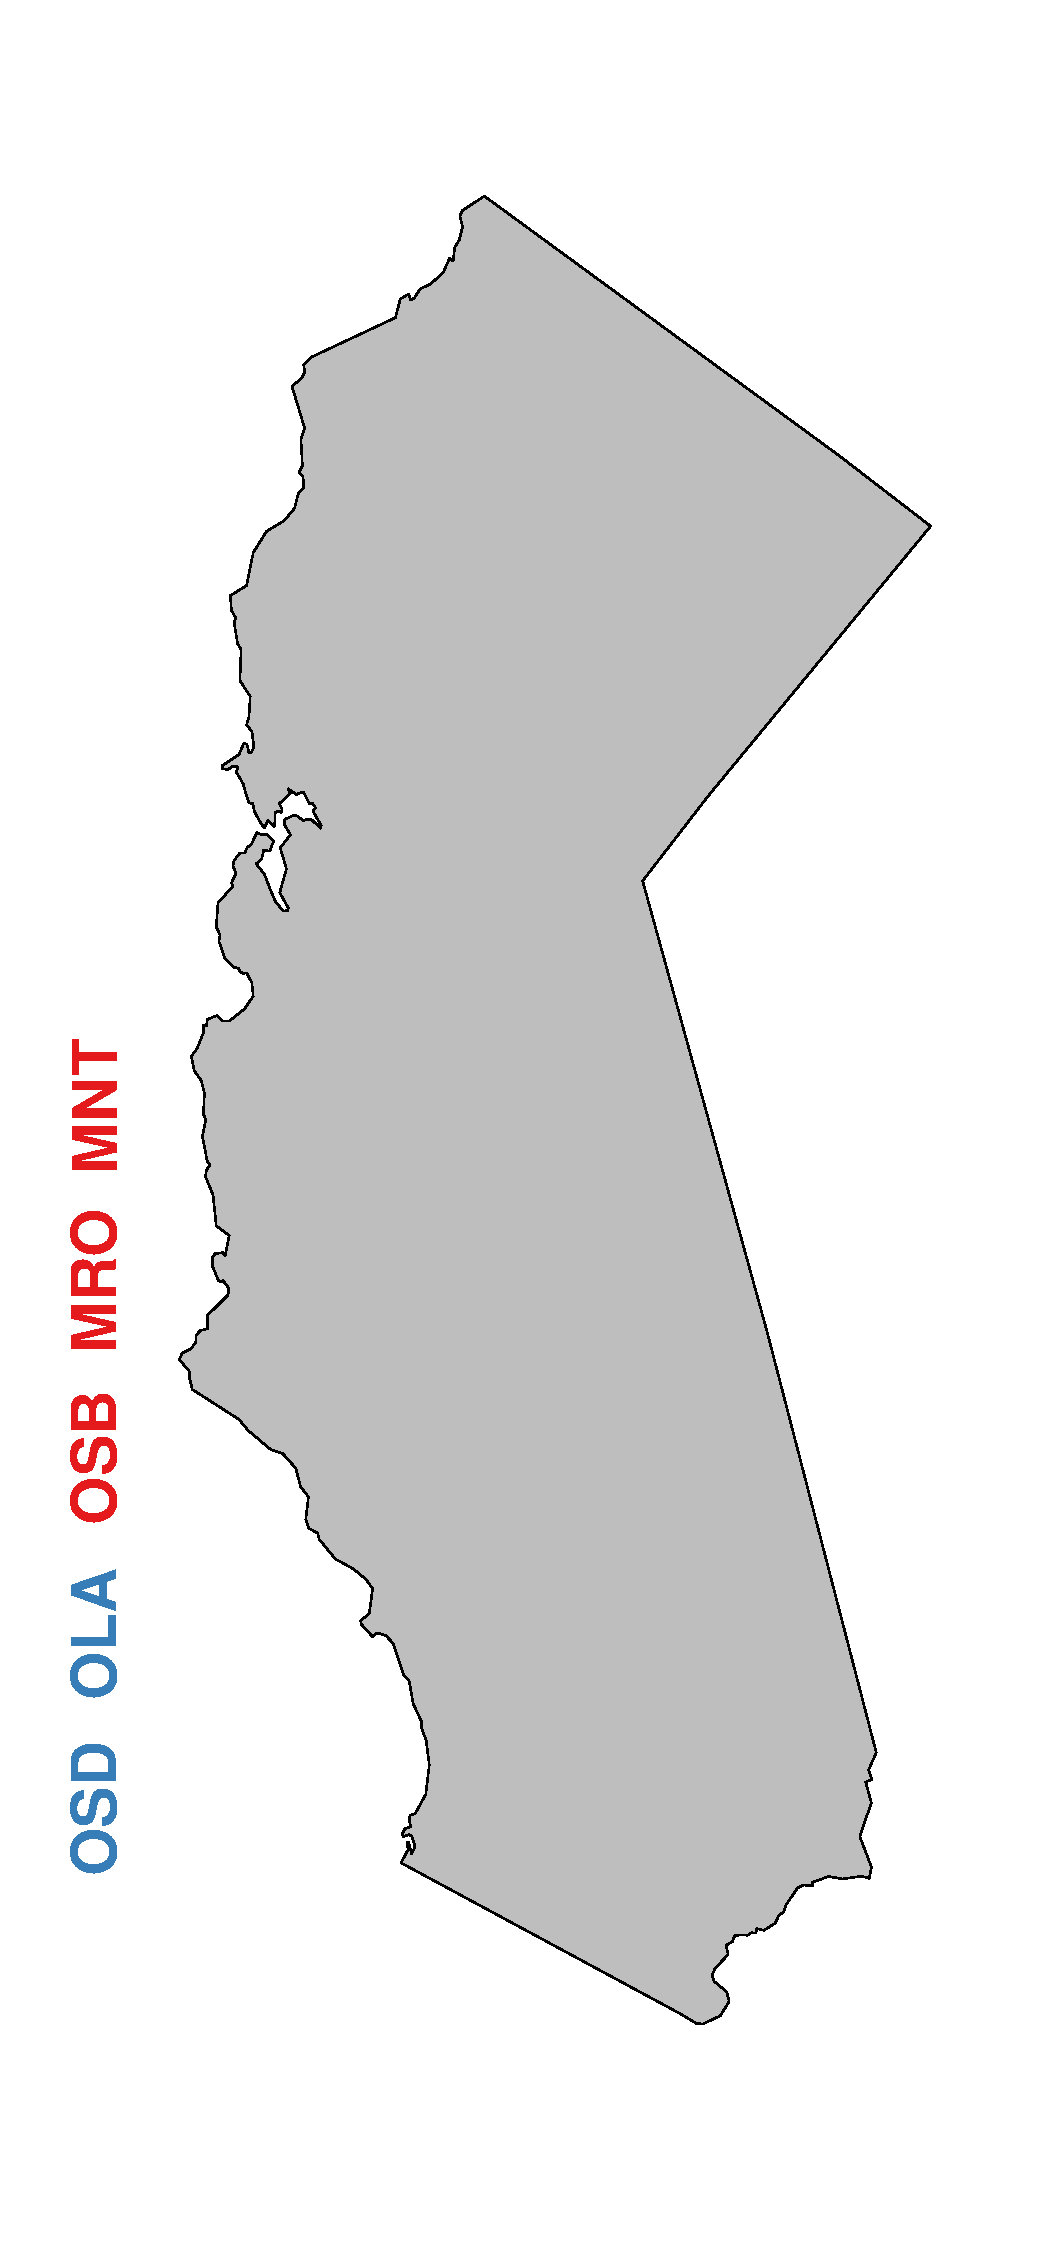
\includegraphics[height=0.37\textheight]{./space4MapBottom.pdf}
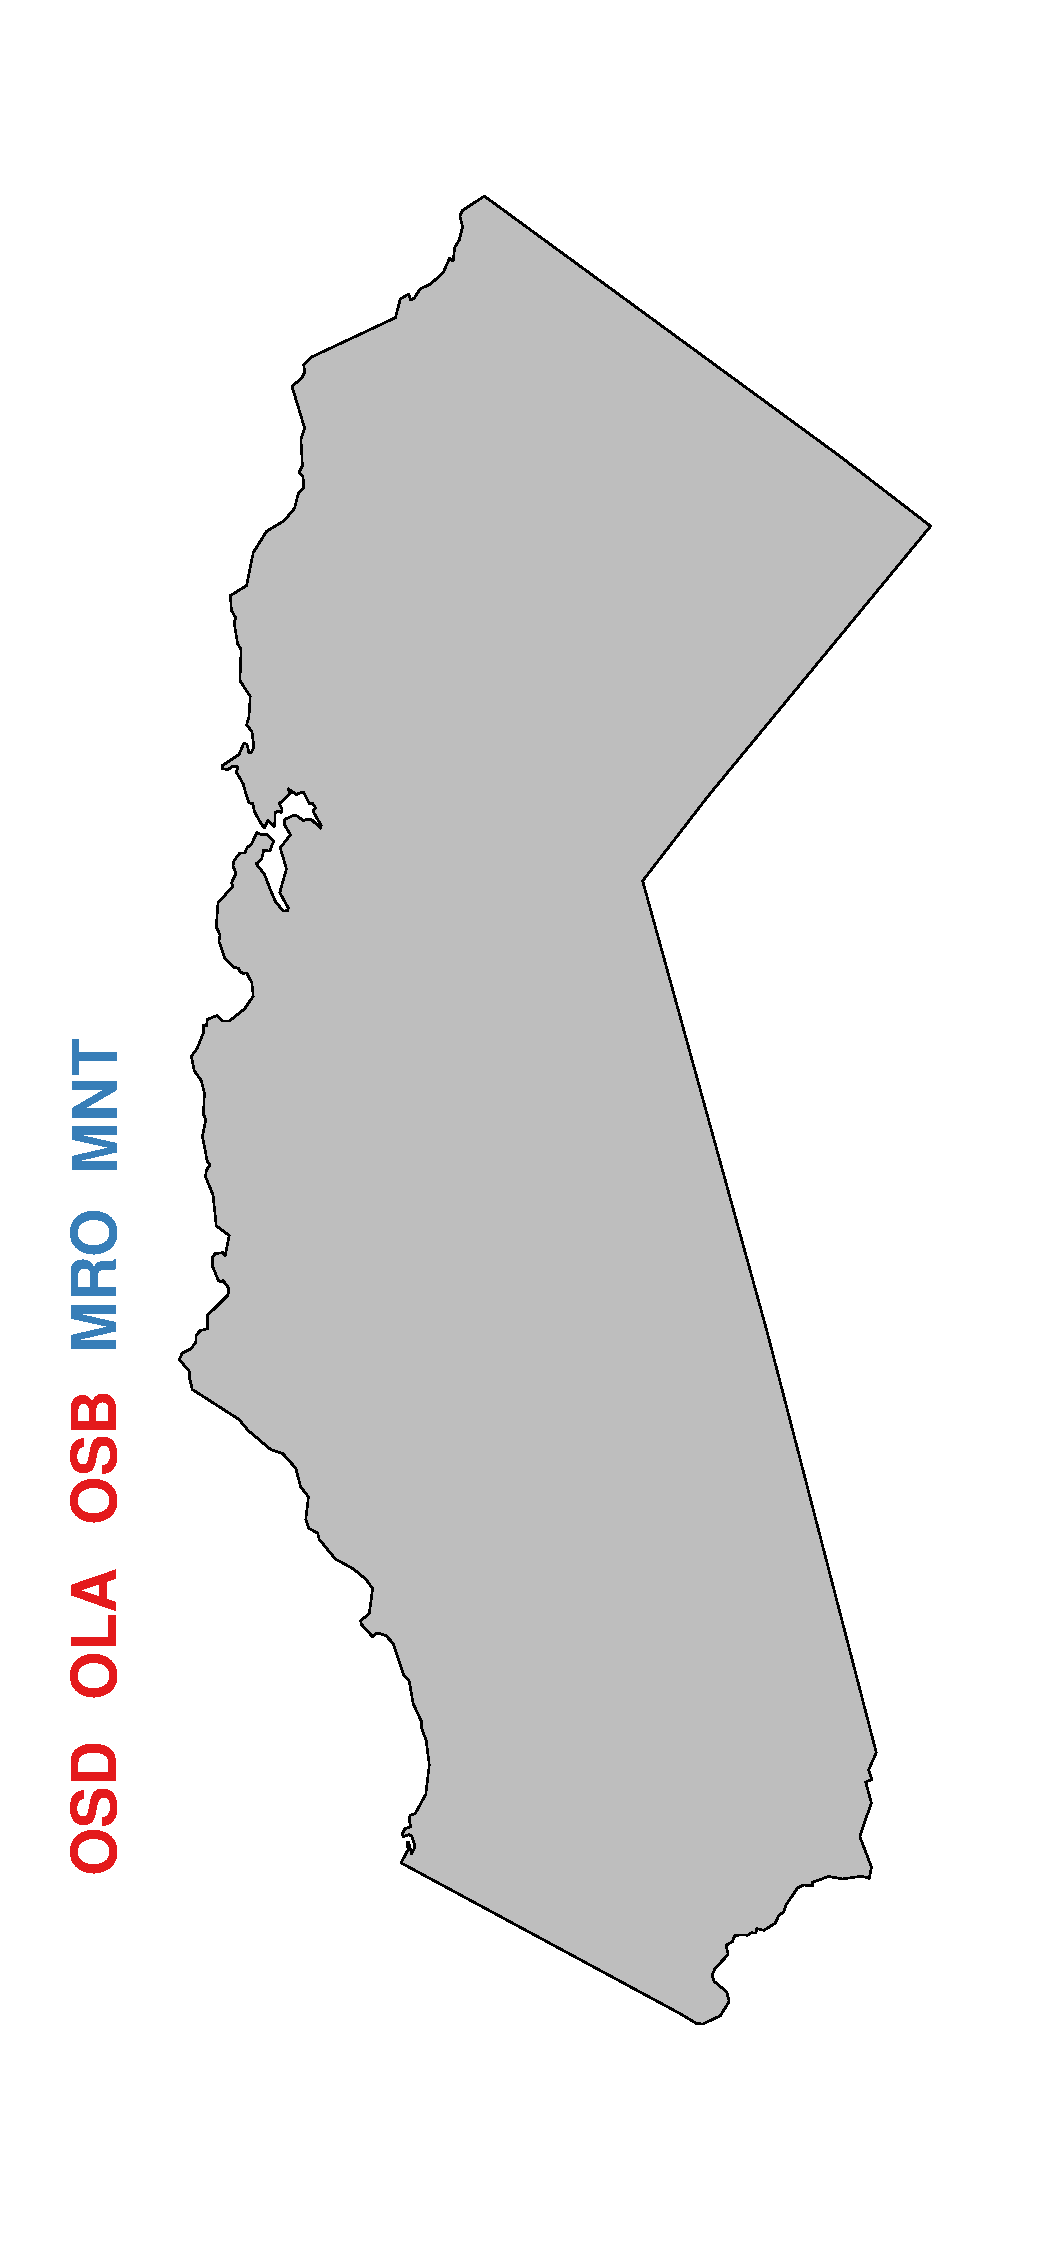
\includegraphics[height=0.37\textheight]{./space5MapBottom.pdf}
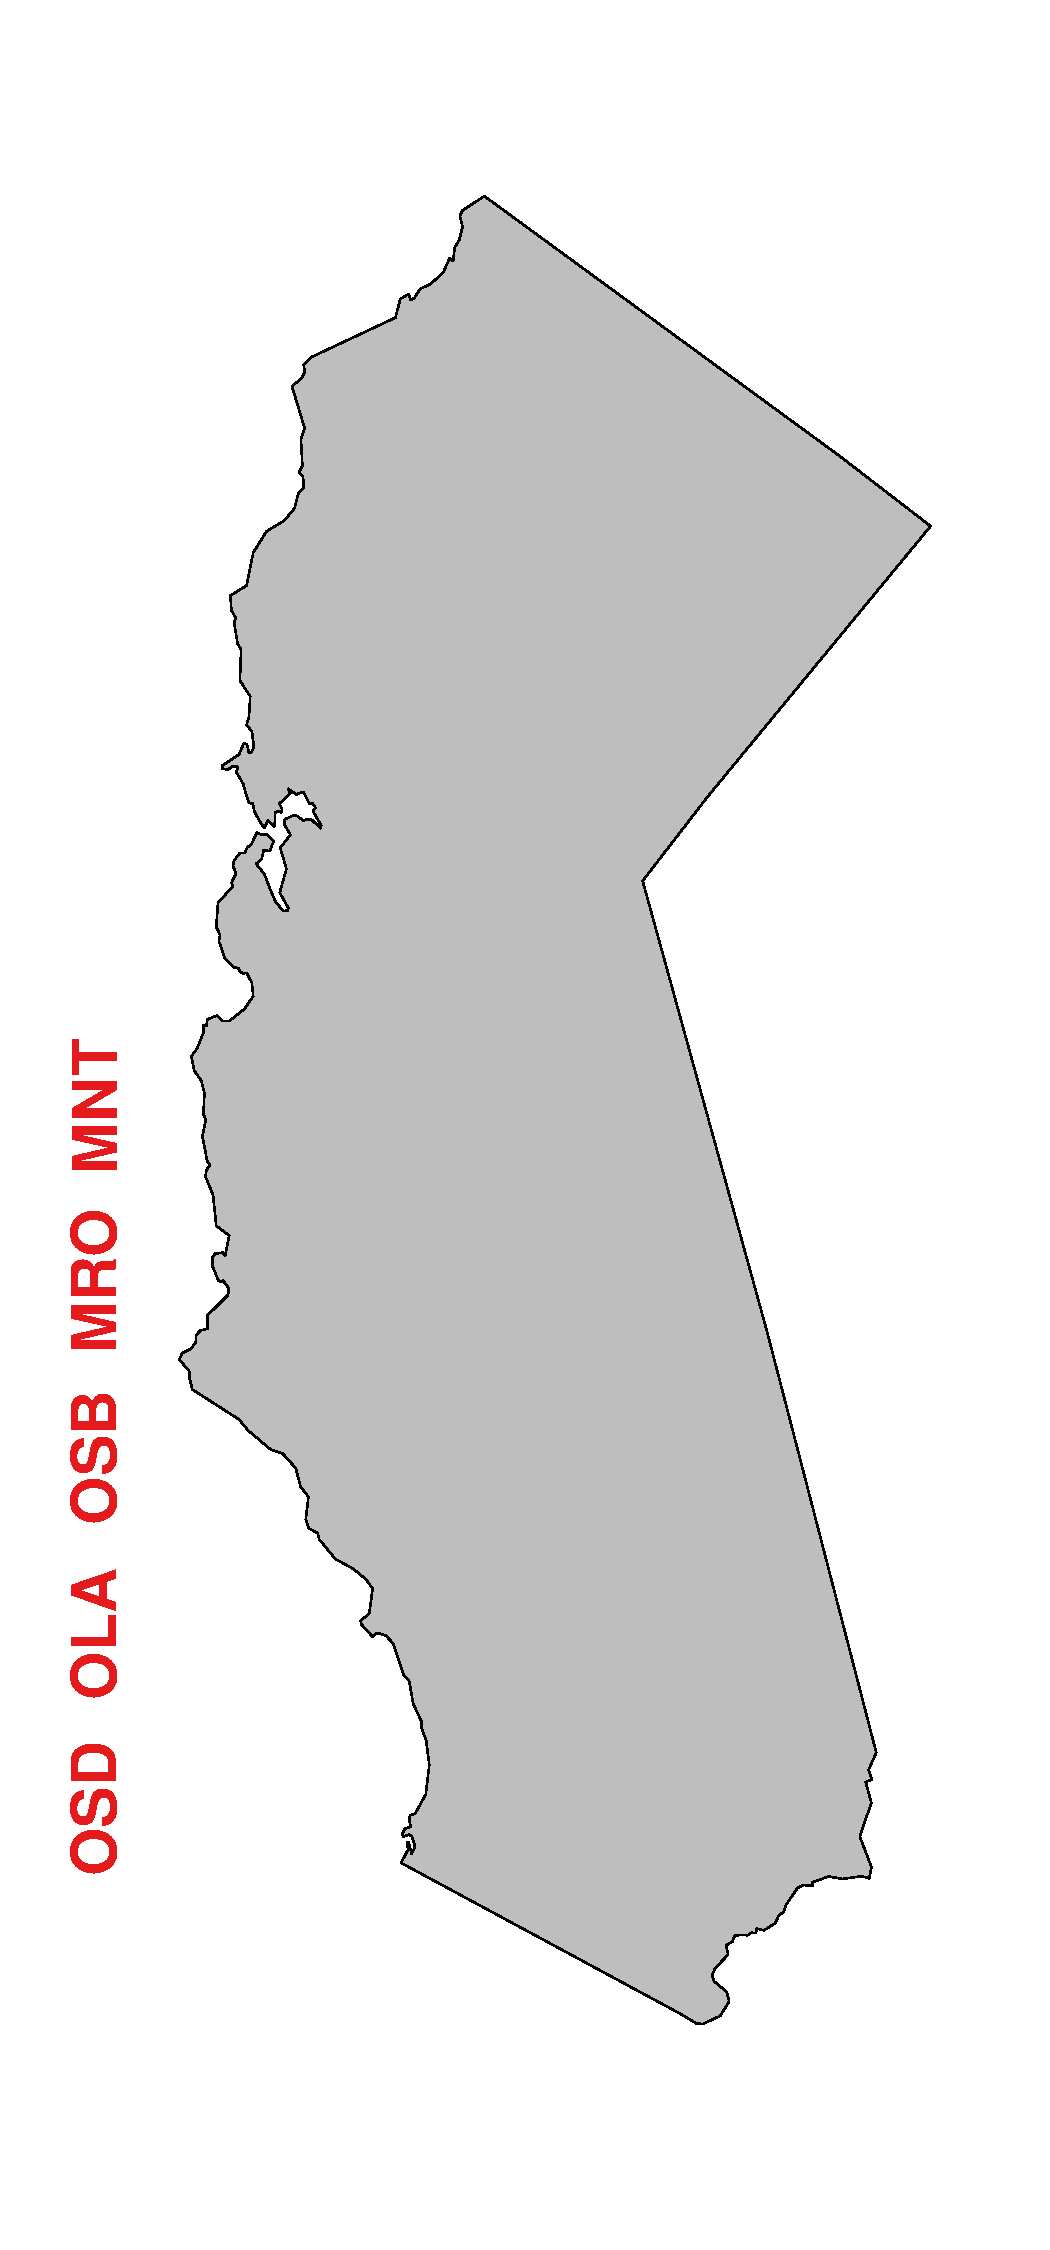
\includegraphics[height=0.37\textheight]{./space1MapBottom.pdf}
\end{frame}

%
%

%\subsection{}
\begin{frame}{Bayesian Model Averaging (BMA)}
      	Consider a set of Models ($M$) indexed by $\iota$: % sharing a common distribution $f(y|\bm{\theta})$:
      	\begin{equation*}
	\omega_\iota = Pr(M_\iota|y) = \frac{ p(y|M_\iota)p(M_\iota) }{ \sum_\iota p(y|M_\iota)p(M_\iota) }
      	%\omega_j = Pr(\mathbb{M}_j|\bm{y}) = \frac{ p(\bm{y}|\mathbb{M}_j)p\cancelto{\propto 1}{(\mathbb{M}_j)} }{ \sum_i p(\bm{y}|\mathbb{M}_i)p\cancelto{\propto 1}{(\mathbb{M}_i)}} = \frac{ p(\bm{y}|\mathbb{M}_j) }{ \sum_i p(\bm{y}|\mathbb{M}_i)}
	\end{equation*}
      	\begin{equation*}
      	\bar p(\bm{\theta}|\bm{y}) = \sum_{\iota} \omega_\iota p(\bm{\theta}|\bm{y}, M_\iota)
      	\end{equation*}
	\indent if $f$ only depends on $M$ through $\bm{\theta}$, then
      	\begin{equation*}
      	\bar p(y^*|\bm{y}) = \bm{\int} f(y^*|\bm{\theta}) \bar p(\bm{\theta}|\bm{y}) \bm{d\theta}
      	\end{equation*}
$~$\\
\fontsize{6pt}{7.2}\selectfont
* Hoeting, J. A., Madigan, D., Raftery, A. E., and Volinsky, C. T. (1999). Bayesian model averaging: a tutorial. \textit{Statistical science}, 382-401.
\end{frame}

%
%

%\subsection{}
\begin{frame}
\centering
\resizebox{1\textwidth}{!}{\begin{tabular}{|c|c|c|c|c|c|c|c|c|c|c|}
        %\hline \multicolumn{6}{|c|}{MCAT 250} \\ \hline
        \hline \multicolumn{11}{|c|}{MCAT 250} \\ \hline
        %$\omega$&0.32&0.14&0.13&0.12&0.02 \\ \hline %&0.02&0.02&0.02&0.02&0.02 \\ \hline
        $\omega$&0.32&0.14&0.13&0.12&0.02&0.02&0.02&0.02&0.02&0.02 \\ \hline
        CRS&\cellcolor[HTML]{E41A1C}&\cellcolor[HTML]{E41A1C}&\cellcolor[HTML]{E41A1C}&\cellcolor[HTML]{E41A1C}&\cellcolor[HTML]{E41A1C}&\cellcolor[HTML]{E41A1C}&\cellcolor[HTML]{E41A1C}&\cellcolor[HTML]{E41A1C}&\cellcolor[HTML]{E41A1C}&\cellcolor[HTML]{E41A1C} \\ \hline%
        ERK&\cellcolor[HTML]{377EB8}&\cellcolor[HTML]{377EB8}&\cellcolor[HTML]{377EB8}&\cellcolor[HTML]{377EB8}&\cellcolor[HTML]{377EB8}&\cellcolor[HTML]{377EB8}&\cellcolor[HTML]{377EB8}&\cellcolor[HTML]{377EB8}&\cellcolor[HTML]{377EB8}&\cellcolor[HTML]{377EB8} \\ \hline%
        BRG&\cellcolor[HTML]{4DAF4A}&\cellcolor[HTML]{4DAF4A}&\cellcolor[HTML]{4DAF4A}&\cellcolor[HTML]{4DAF4A}&\cellcolor[HTML]{4DAF4A}&\cellcolor[HTML]{4DAF4A}&\cellcolor[HTML]{4DAF4A}&\cellcolor[HTML]{4DAF4A}&\cellcolor[HTML]{4DAF4A}&\cellcolor[HTML]{4DAF4A} \\ \hline%
        BDG&\cellcolor[HTML]{4DAF4A}&\cellcolor[HTML]{4DAF4A}&\cellcolor[HTML]{4DAF4A}&\cellcolor[HTML]{4DAF4A}&\cellcolor[HTML]{4DAF4A}&\cellcolor[HTML]{4DAF4A}&\cellcolor[HTML]{4DAF4A}&\cellcolor[HTML]{984EA3}&\cellcolor[HTML]{4DAF4A}&\cellcolor[HTML]{4DAF4A} \\ \hline%
        OSF&\cellcolor[HTML]{984EA3}&\cellcolor[HTML]{984EA3}&\cellcolor[HTML]{984EA3}&\cellcolor[HTML]{984EA3}&\cellcolor[HTML]{4DAF4A}&\cellcolor[HTML]{4DAF4A}&\cellcolor[HTML]{4DAF4A}&\cellcolor[HTML]{984EA3}&\cellcolor[HTML]{4DAF4A}&\cellcolor[HTML]{4DAF4A} \\ \hline%
        MNT&\cellcolor[HTML]{984EA3}&\cellcolor[HTML]{984EA3}&\cellcolor[HTML]{984EA3}&\cellcolor[HTML]{984EA3}&\cellcolor[HTML]{984EA3}&\cellcolor[HTML]{984EA3}&\cellcolor[HTML]{984EA3}&\cellcolor[HTML]{FF7F00}&\cellcolor[HTML]{984EA3}&\cellcolor[HTML]{984EA3} \\ \hline%
        MRO&\cellcolor[HTML]{984EA3}&\cellcolor[HTML]{984EA3}&\cellcolor[HTML]{984EA3}&\cellcolor[HTML]{984EA3}&\cellcolor[HTML]{984EA3}&\cellcolor[HTML]{984EA3}&\cellcolor[HTML]{984EA3}&\cellcolor[HTML]{FF7F00}&\cellcolor[HTML]{984EA3}&\cellcolor[HTML]{984EA3} \\ \hline%
        OSB&\cellcolor[HTML]{FF7F00}&\cellcolor[HTML]{FF7F00}&\cellcolor[HTML]{FF7F00}&\cellcolor[HTML]{FF7F00}&\cellcolor[HTML]{FF7F00}&\cellcolor[HTML]{FF7F00}&\cellcolor[HTML]{FF7F00}&\cellcolor[HTML]{FF7F00}&\cellcolor[HTML]{984EA3}&\cellcolor[HTML]{FF7F00} \\ \hline%
        OLA&\cellcolor[HTML]{FF7F00}&\cellcolor[HTML]{FFFF33}&\cellcolor[HTML]{FF7F00}&\cellcolor[HTML]{FFFF33}&\cellcolor[HTML]{FF7F00}&\cellcolor[HTML]{FFFF33}&\cellcolor[HTML]{FFFF33}&\cellcolor[HTML]{FFFF33}&\cellcolor[HTML]{FF7F00}&\cellcolor[HTML]{FF7F00} \\ \hline%
        OSD&\cellcolor[HTML]{FF7F00}&\cellcolor[HTML]{FFFF33}&\cellcolor[HTML]{FFFF33}&\cellcolor[HTML]{A65628}&\cellcolor[HTML]{FFFF33}&\cellcolor[HTML]{FFFF33}&\cellcolor[HTML]{A65628}&\cellcolor[HTML]{FFFF33}&\cellcolor[HTML]{FFFF33}&\cellcolor[HTML]{FF7F00} \\ \hline%
\end{tabular}}
\end{frame}

%
%

%\subsection{}
\begin{frame}
\color{red} select port pooling results
\end{frame}

\begin{frame}
\begin{itemize}
\item {\color{red}Red stuff}
\item Species Composition Proof
\end{itemize}
\end{frame}


%%
%\section{Performance}
%\subsection{}
%\begin{frame}
%\end{frame}

%
%

%
\section{Extra}
\subsection{}
\begin{frame}
\centering
%\vspace{-1.2cm}
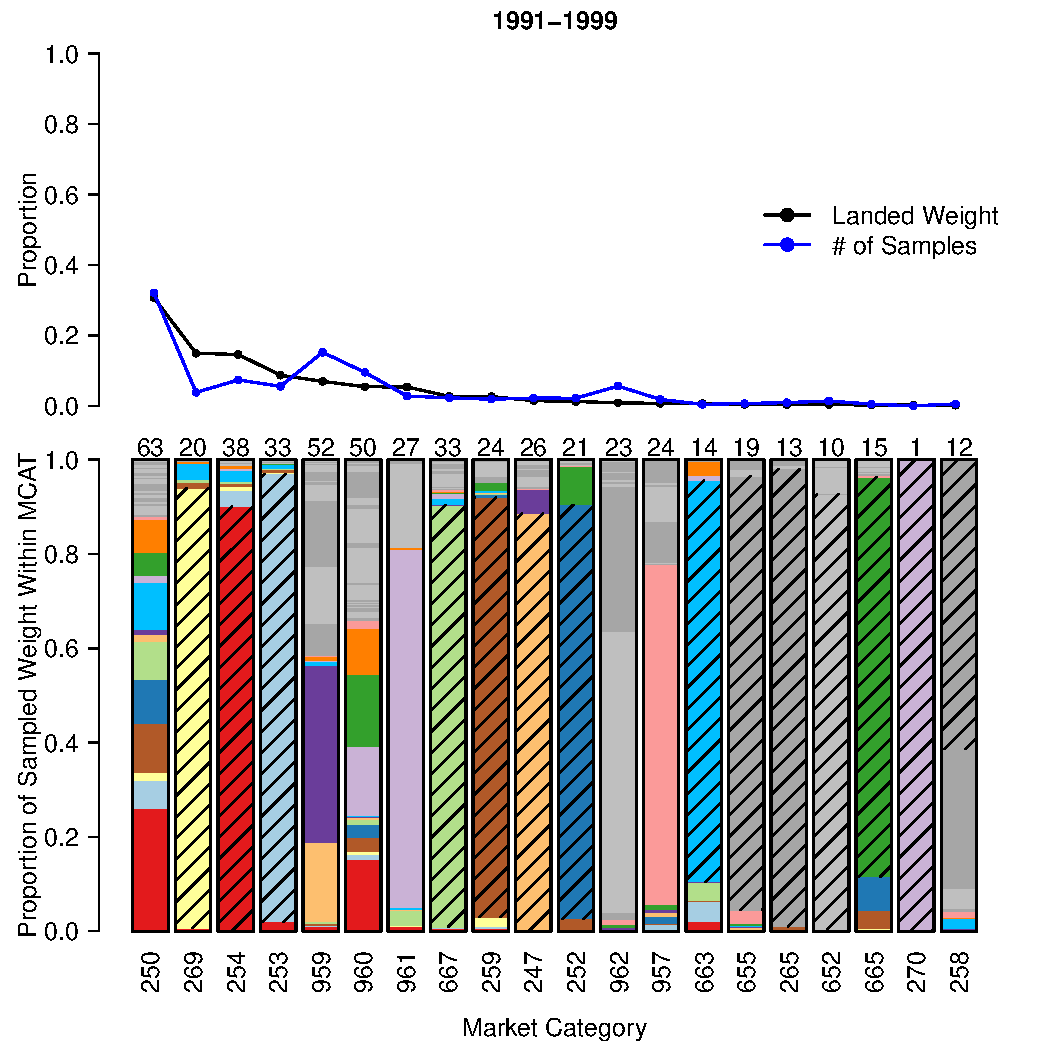
\includegraphics[height=\textheight]{../pictures/1991to1999Bar3.pdf}
%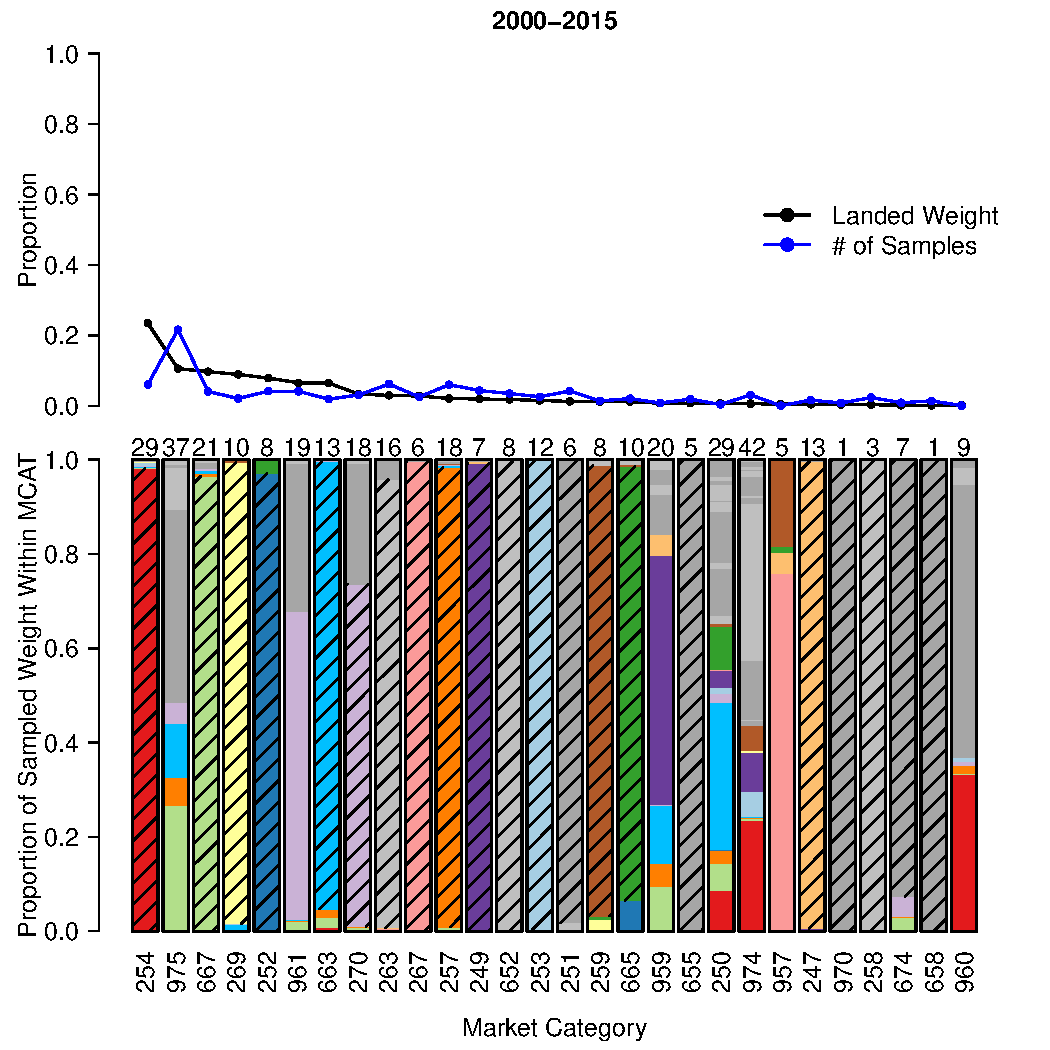
\includegraphics[width=0.43\textwidth]{../pictures/2000to2015Bar3.pdf}
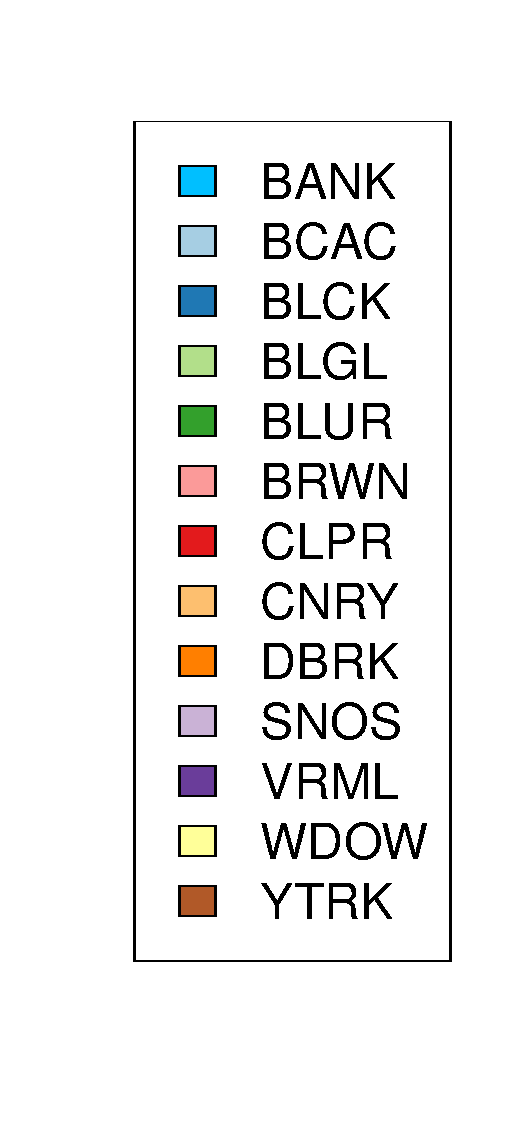
\includegraphics[height=\textheight]{../pictures/barplotLegend.pdf}
\end{frame}

%
%

%
\subsection{}
\begin{frame}
\centering
%\vspace{-1.2cm}
%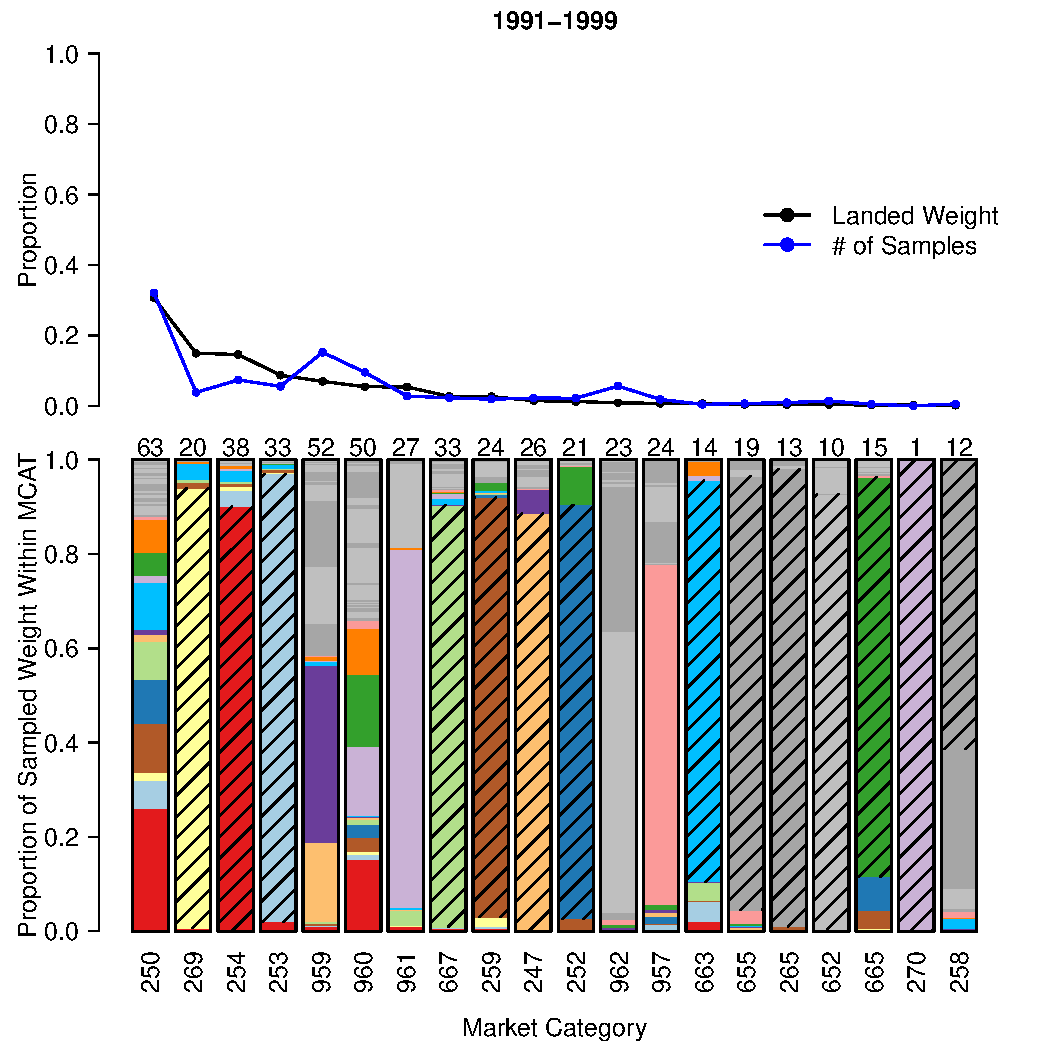
\includegraphics[height=\textheight]{../pictures/1991to1999Bar3.pdf}
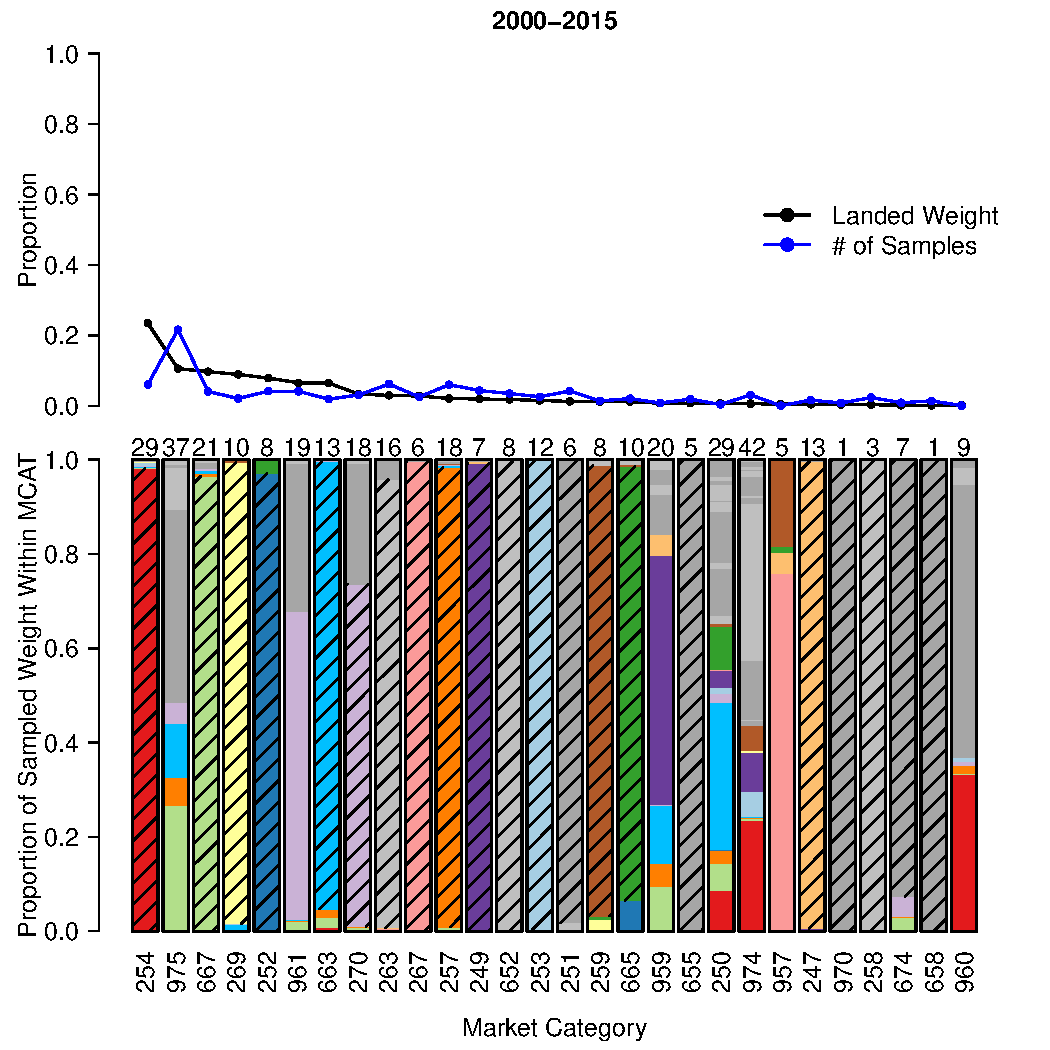
\includegraphics[height=\textheight]{../pictures/2000to2015Bar3.pdf}
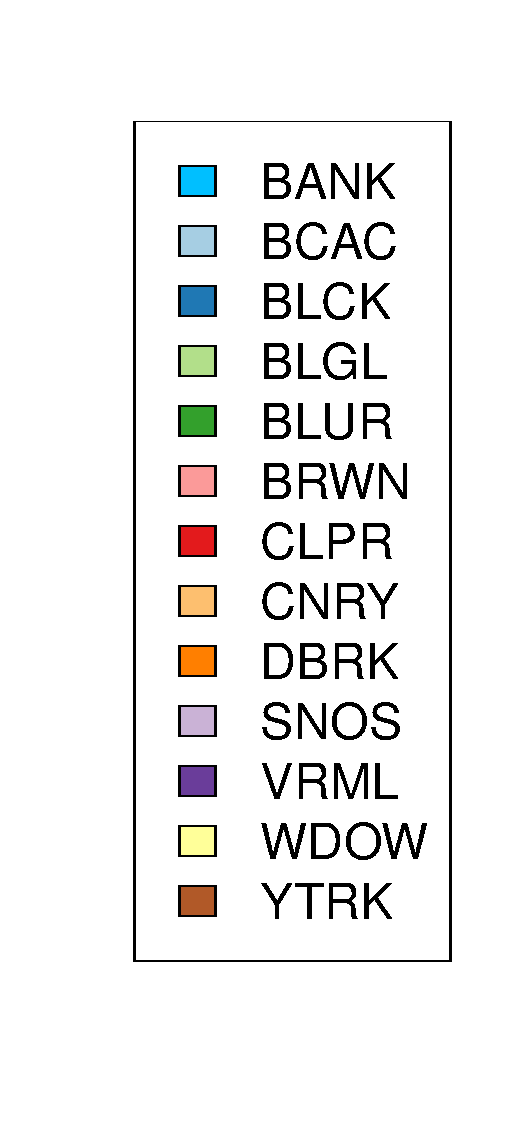
\includegraphics[height=\textheight]{../pictures/barplotLegend.pdf}
\end{frame}


%%
%%
%
%%\section{Introduction}
%%\subsection{}
%%
%%12*4/3 = 16
%%
%
%%
%\section{Modeling}
%\subsection{}
%\begin{frame}{Market Category Stratification}%{\color{red}Observed Rockfish Market Categories}}%\color{red}(add other orange and other blue n
%       \hspace*{-0.75cm}
%       \includegraphics[width=1.1\textwidth, height=0.5\textheight]{./propCatchCrop.png}\\
%       \vspace{-0.9cm}
%       \hspace*{-0.9cm}
%       \includegraphics[width=1.16\textwidth, height=0.5\textheight]{./nMcatsEMA.pdf}
%       %\includegraphics[width=1\textwidth]{./colorPic.jpg}
%       %$~$
%       %\hspace*{-1cm}
%       %\vspace*{-3cm}
%\end{frame}
%
%%
%%
%
%%\subsection{}
%\begin{frame}{Sampling Effort}
%       \hspace*{-0.75cm}
%       \includegraphics[width=1.1\textwidth, height=0.5\textheight]{./sampleNumTotalCrop.png}\\
%       \vspace{-0.9cm}
%       \hspace*{-0.9cm}
%       \includegraphics[width=1.16\textwidth, height=0.5\textheight]{./stratAvgSamp.pdf}
%\end{frame}
%
%%
%%
%
%%%\subsection{}
%%\begin{frame}{Borrowing Strategies}%How to Tell the old/new story: How to try all partitions and see what happens; (Bias/Variance Trade-off)}
%%%0.24
%%\hspace{0.5cm}
%%\begin{minipage}[h!]{0.2\textwidth}
%%        \hspace*{-0.5cm}
%%        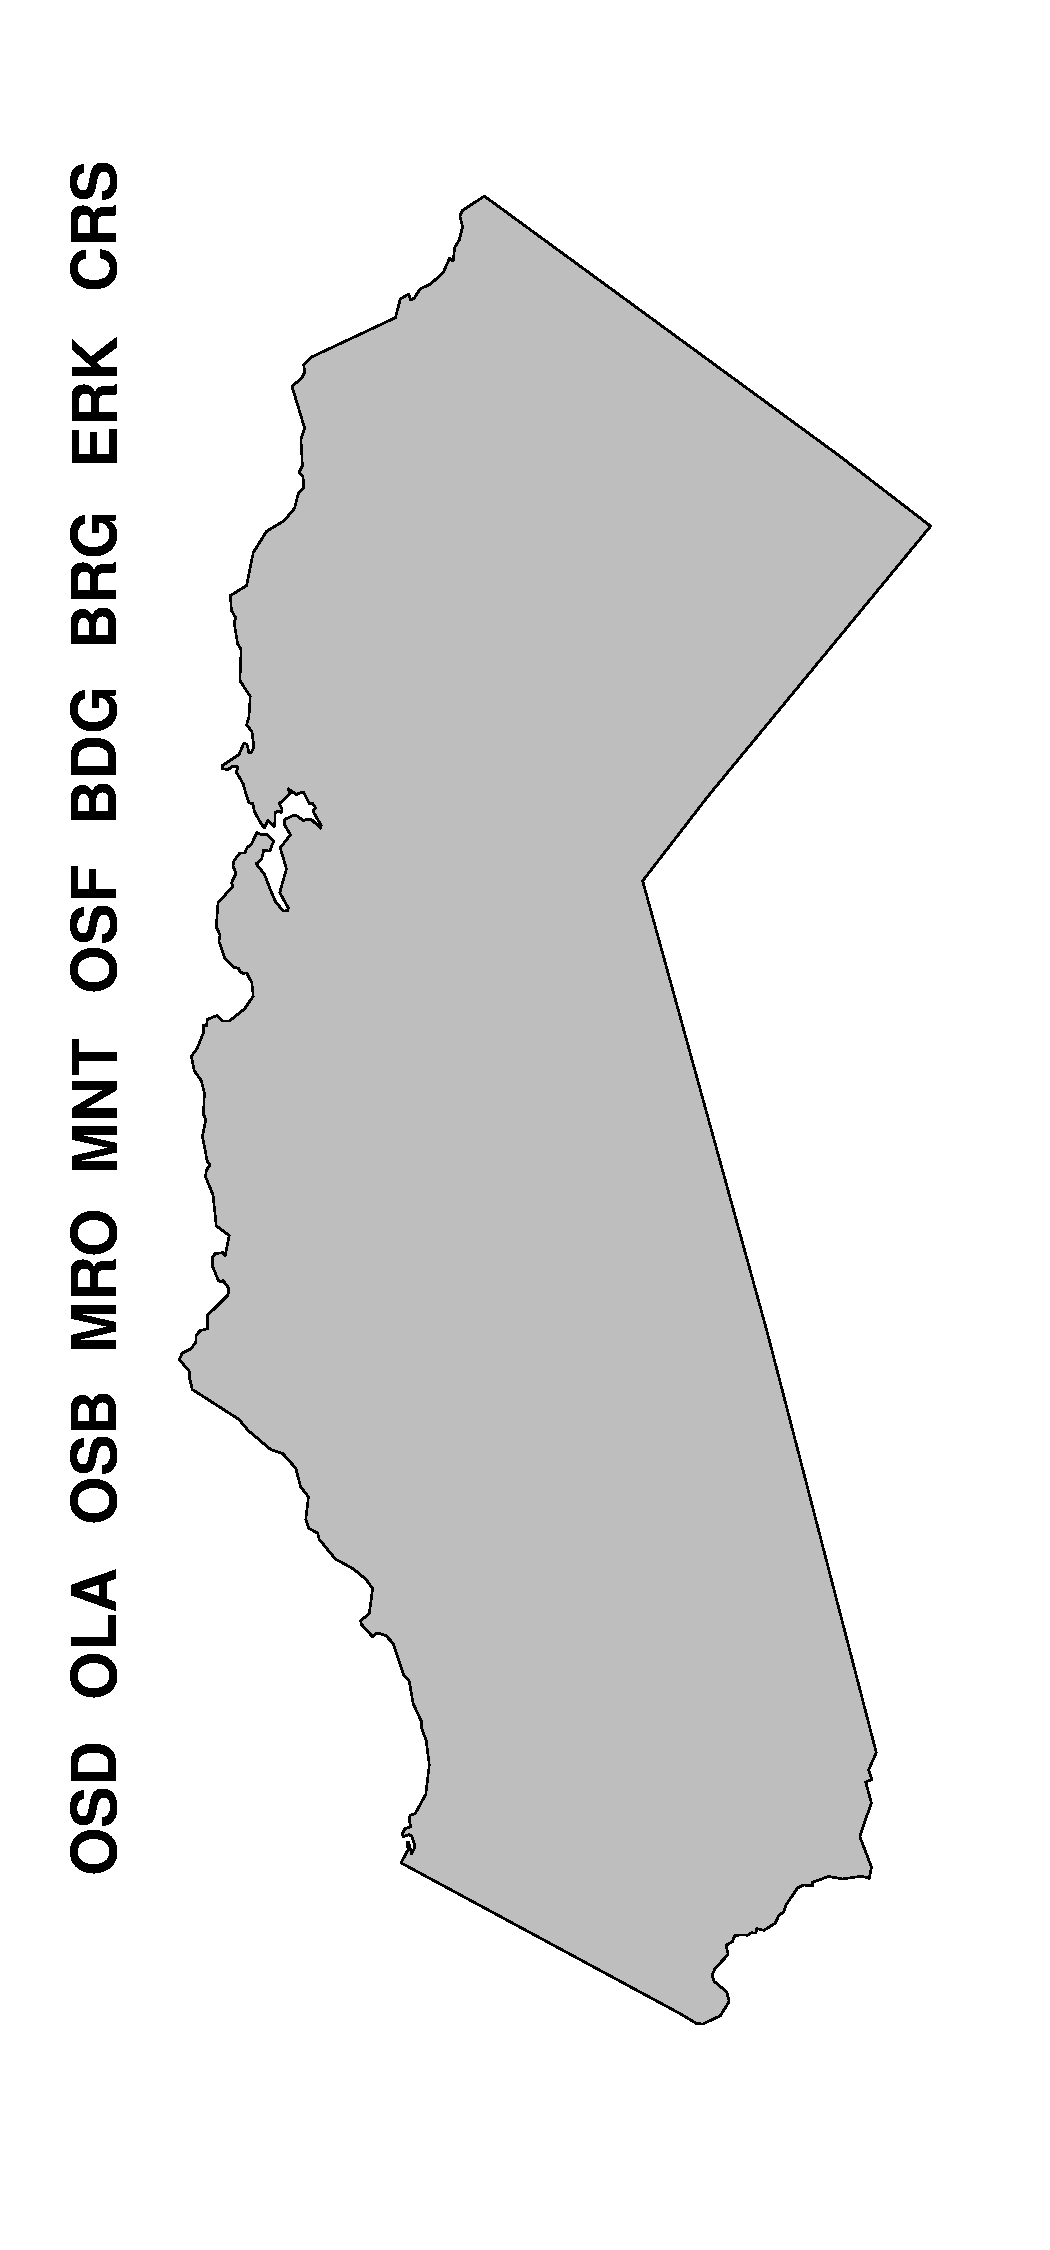
\includegraphics[width=1.2\textwidth]{mapFullBlank.pdf}
%%\end{minipage}
%%\begin{minipage}[h!]{0.2\textwidth}
%%        \hspace*{-0.25cm}
%%        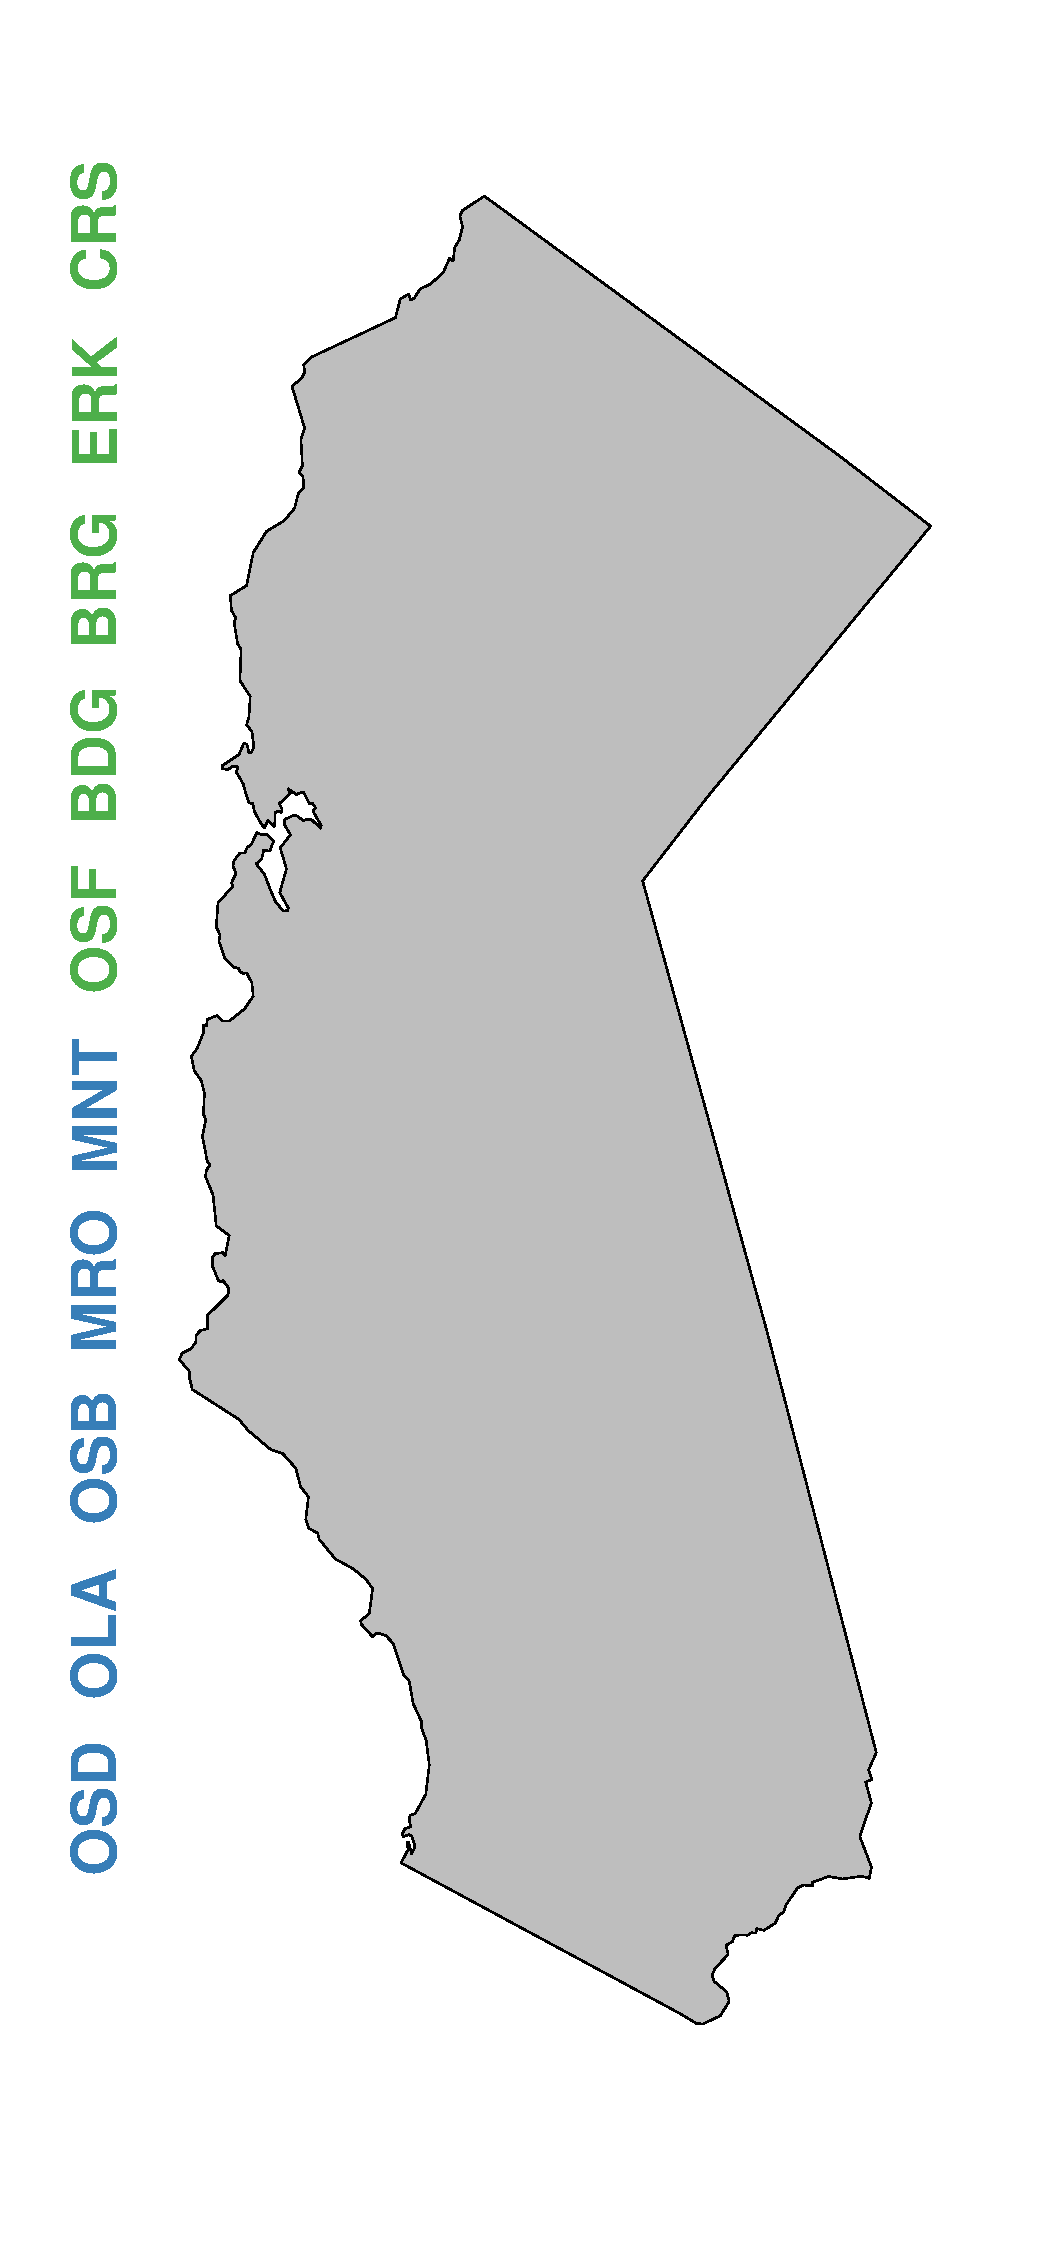
\includegraphics[width=1.2\textwidth]{mapFullHalfHalf.pdf}
%%\end{minipage}
%%\begin{minipage}[h!]{0.2\textwidth}
%%        \hspace*{0.25cm}
%%        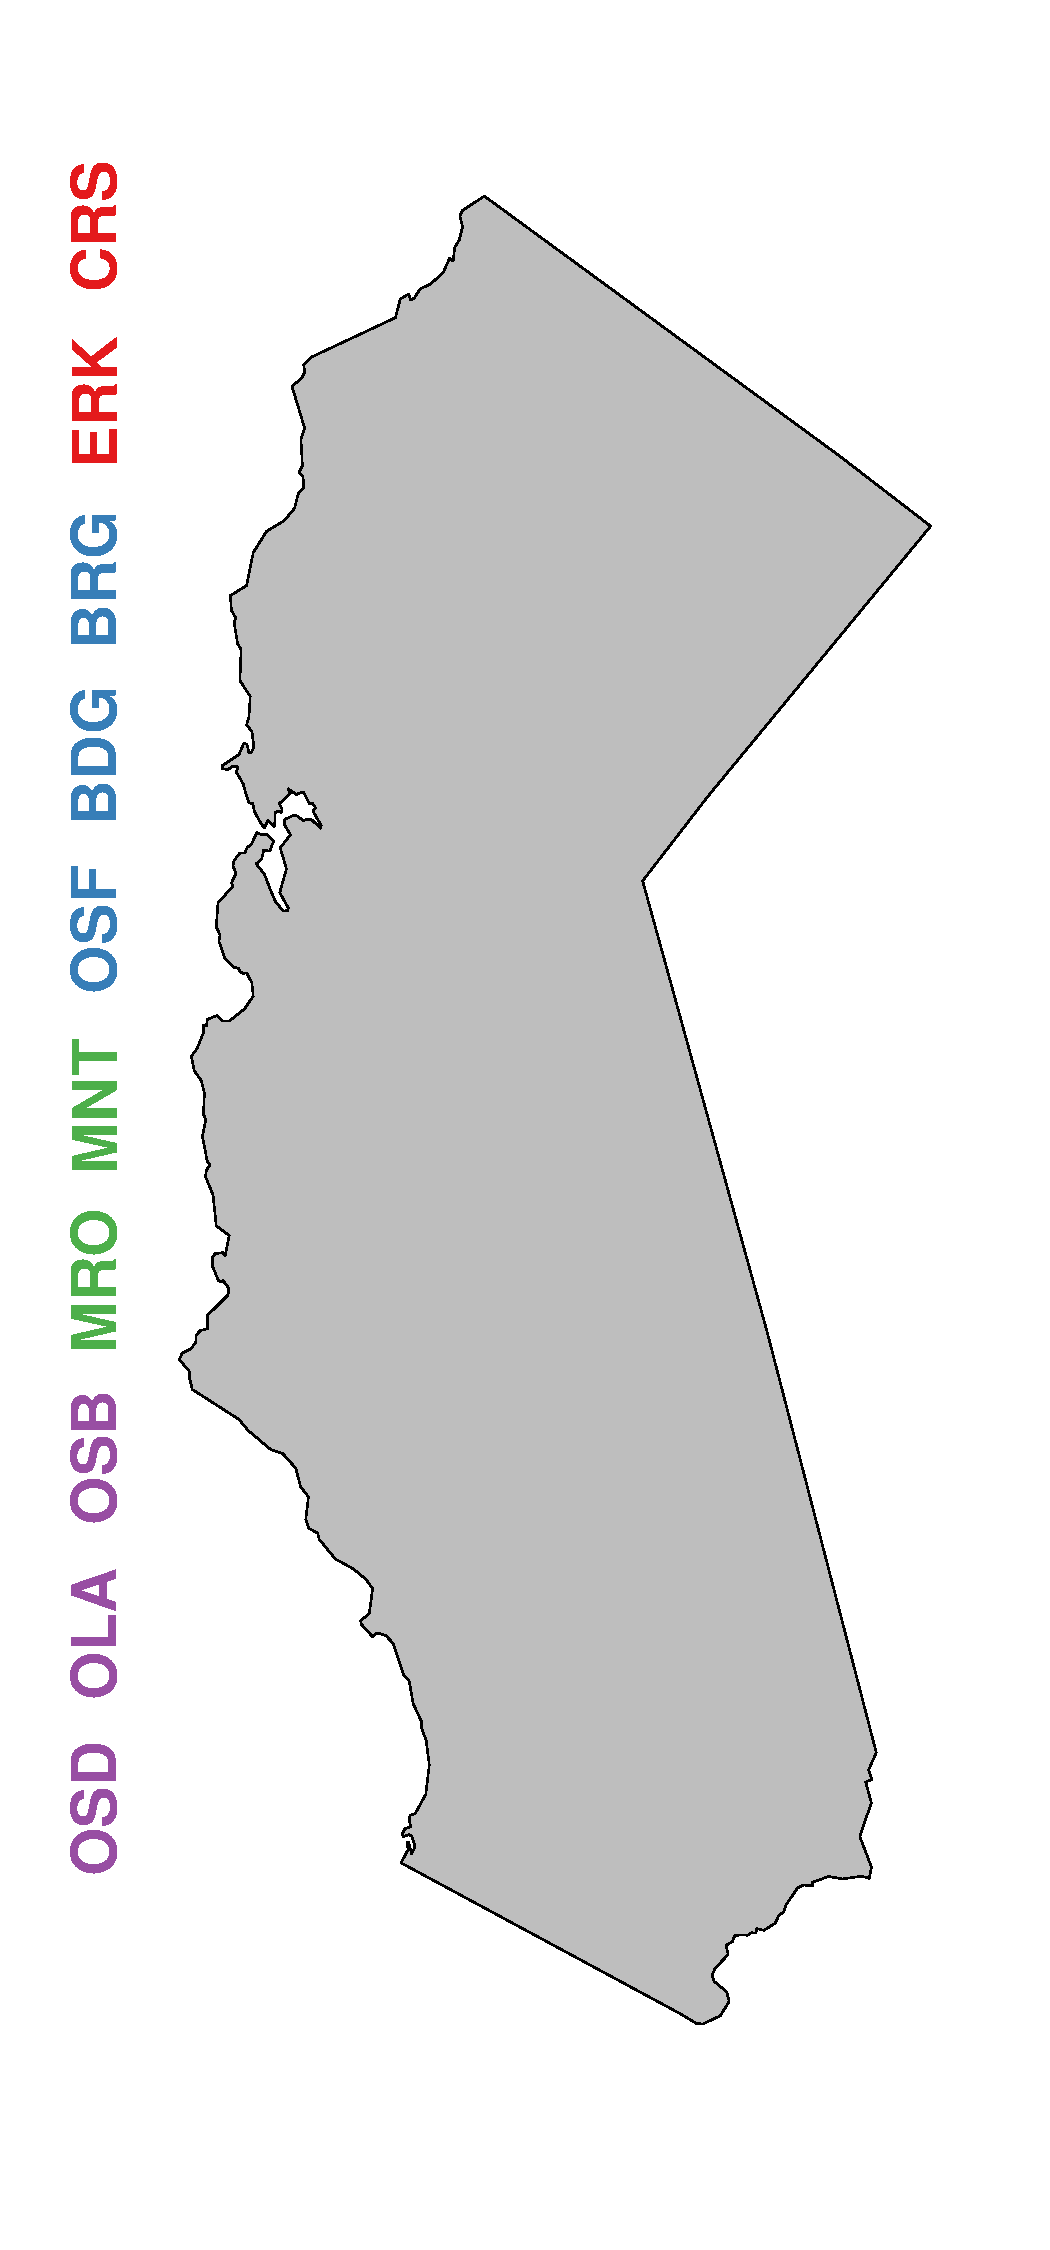
\includegraphics[width=1.2\textwidth]{mapFullConcMend.pdf}
%%\end{minipage}
%%%\begin{minipage}[h!]{0.19\textwidth}
%%%        \hspace*{0.25cm}
%%%        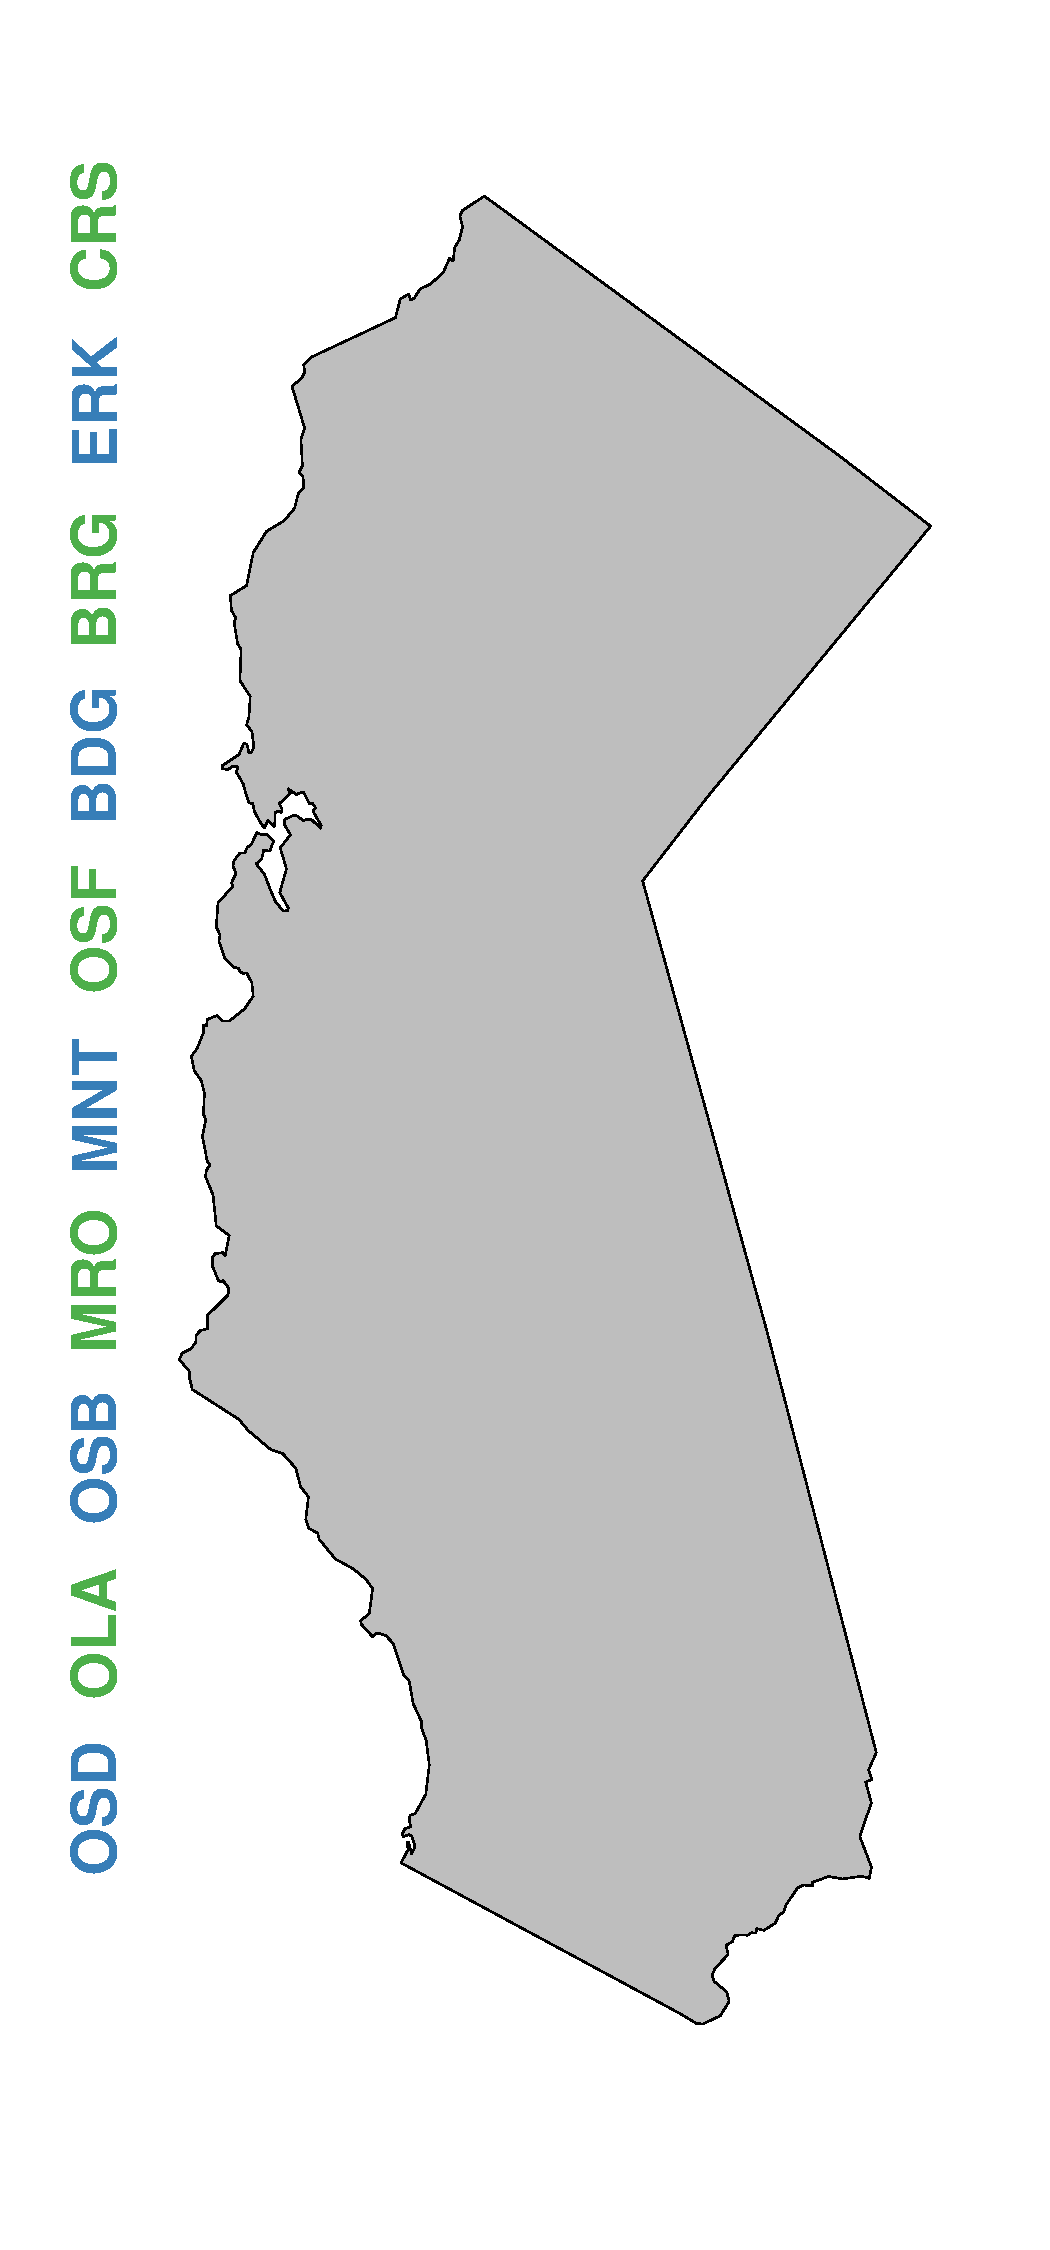
\includegraphics[width=1.2\textwidth]{mapFullEveryOther.pdf}
%%%\end{minipage}
%%\begin{minipage}[h!]{0.2\textwidth}
%%        \hspace*{0.5cm}                %1.2
%%        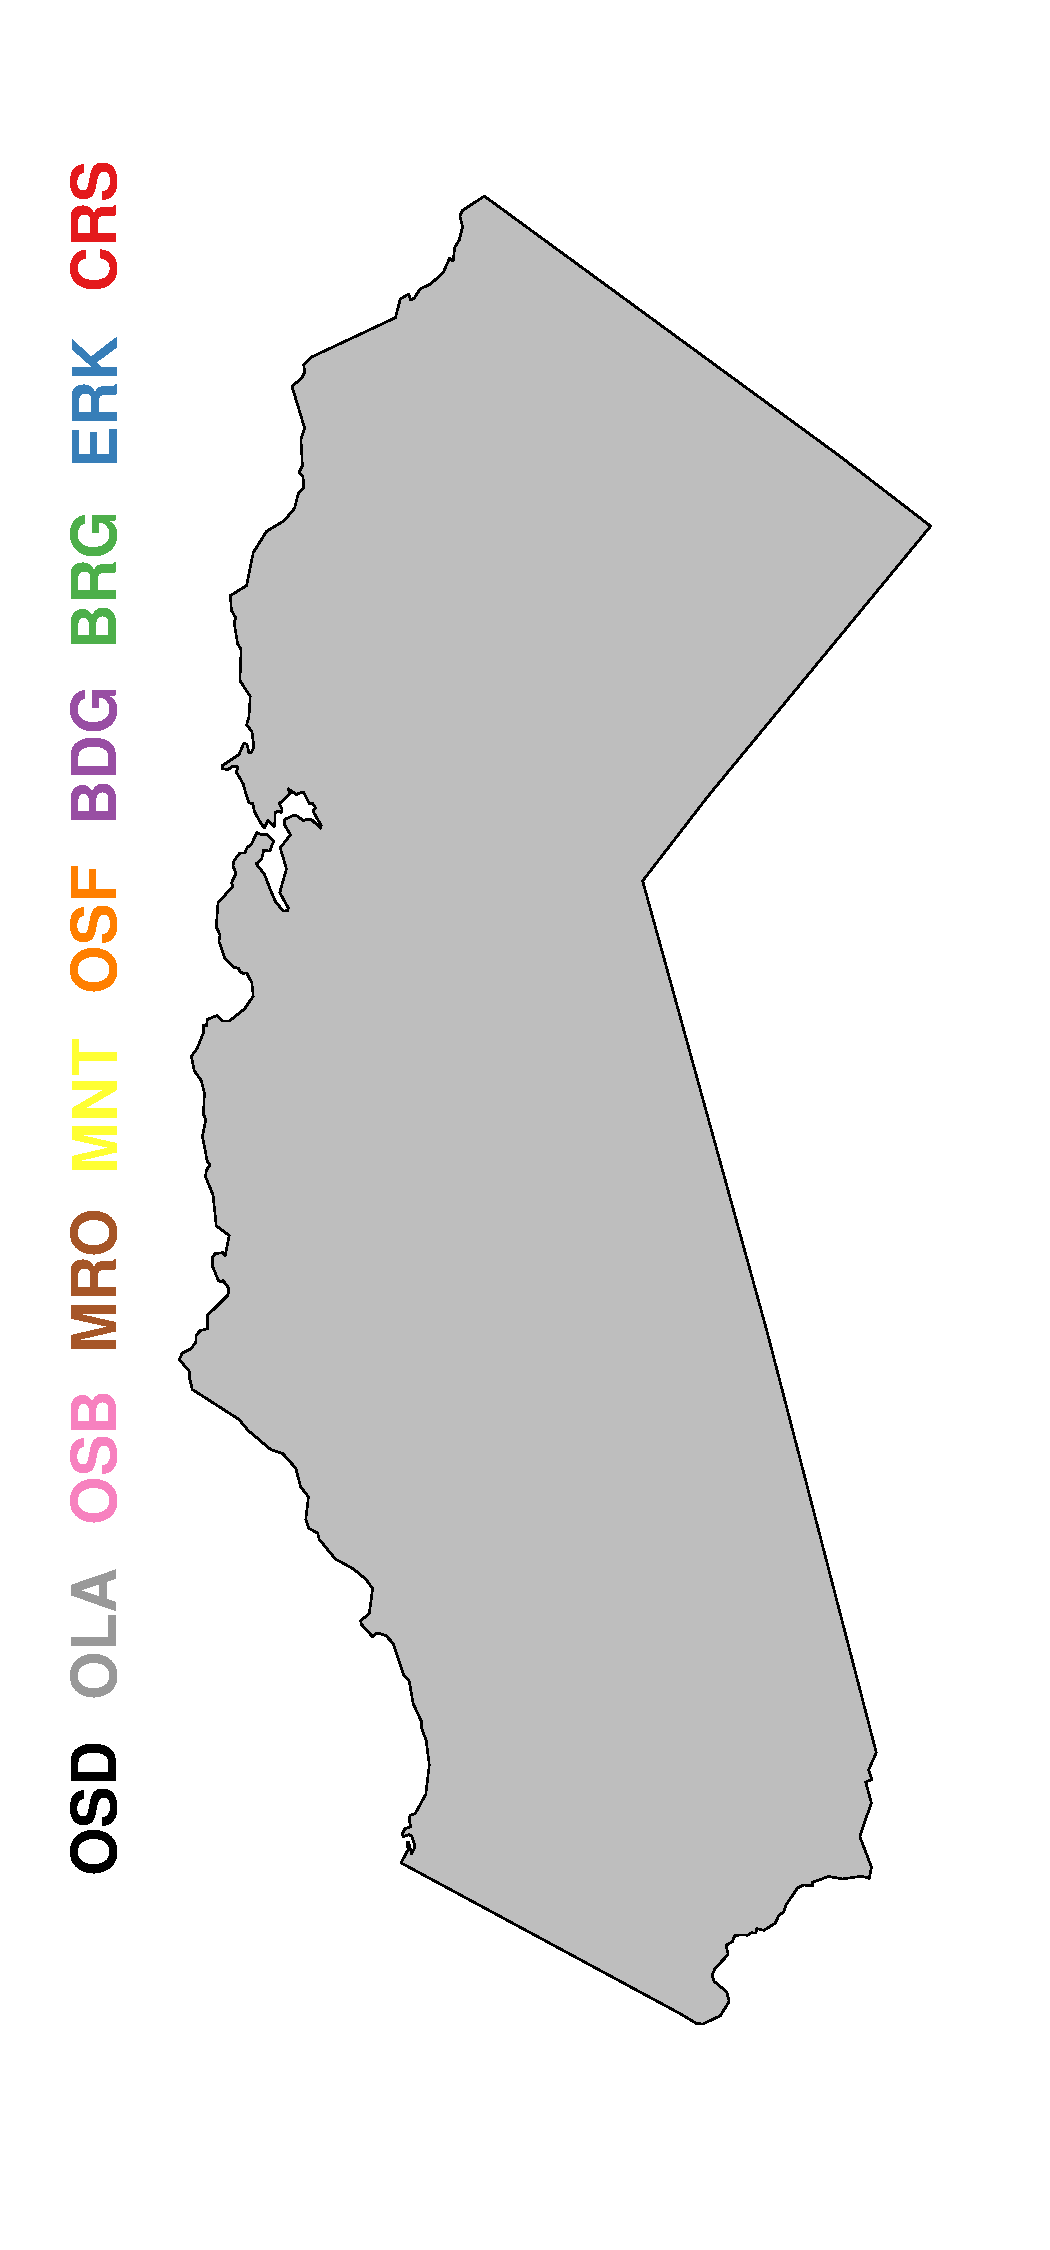
\includegraphics[width=1.2\textwidth]{mapFullSparse.pdf}
%%\end{minipage}
%%\vspace{-0.5cm}
%%\begin{equation*}
%%\text{MSE}(\hat\theta) = \mathbb{E}\left[~(\hat\theta - \theta)^2~\right] = \overbrace{\mathbb{E}\Big[~\left(\hat\theta-\mathbb{E}(\hat\theta)\right)^2~\Big]}^{\text{Var}(\hat \theta)} + \overbrace{\Big(~\mathbb{E}(\hat\theta)-\theta~\Big)^2}^{\text{Bias}(\hat \theta, \theta)^2}
%%\end{equation*}
%%\end{frame}
%
%
%%%
%%%
%%
%%\subsection{}
%%\begin{frame}{Modeling Concerns}
%%\begin{itemize}
%%	\setlength\itemsep{0.25cm}
%%	\item[] \hspace*{-0.5cm} {\color{blue} $\mathbf{\substack{\text{Port Sampling}\\\text{(Counts)}}}$ $\rightarrow$ $\mathbf{\substack{\text{Species Composition}\\\text{(Proportion)}}}$}\\
%%	\begin{itemize}
%%		\setlength\itemsep{0.25cm} 
%%		\item Multinomial Model
%%		\item Poisson $\rightarrow$ Multinomial
%%		%\item Samplers are Slow
%%	\end{itemize}
%%	\item[] \hspace*{0cm} {\color{blue} $\mathbf{\substack{\text{Sparse}\\\text{Sampling}}}$ $\rightarrow$ $\mathbf{\substack{\text{Degenerate}\\\text{Asymtoptics}}}$}\\
%%	\begin{itemize}
%%		\setlength\itemsep{0.25cm}
%%		%\item Degenerate Asymtoptics
%%		\item Stratum Pooling
%%		\item Hierarchical Modeling	
%%	\end{itemize}	
%%	\item[] \hspace*{0cm} {\color{blue}Overdispersion }
%%	\begin{itemize}
%%		\item Poisson $=>$ Negative Binomial	
%%		\item Dirichlet-Multinomial
%%		\begin{itemize}
%%			\item Samplers are Slooow
%%			\item Beta-Binomial
%%		\end{itemize}
%%	\end{itemize}
%%%		\item handles overdispersion
%%%		\item no multinomial-negative binomial transformation 
%%%		\item independent models of weight fit via inla are fast
%%%		\item prediction and normalization $=>$ sppComp
%%%	\end{itemize}
%%%	\item Dirichlet-Multinomial
%%%	\begin{itemize}
%%%                \item hard to fit with these data. 
%%%                \item Asymtoptics out the door.
%%%                \item Samplers are realllly slow.
%%%		\item handles overdispersion
%%%        \end{itemize}
%%%	\item direct analogy to Beta-Binomial rather than Negative Binomial
%%%	\begin{itemize}
%%%		\item waic example comparison
%%%                \item handles overdispersion 
%%%                \item independent models of weight fit via inla are fast
%%%                \item prediction and normalization $=>$ sppComp
%%%        \end{itemize}
%%\end{itemize}
%%\end{frame}
%%
%%%
%%%
%
%%
%\subsection{}
%\begin{frame}
%\vspace{-0.5cm}
%\hspace{-0.5cm}
%\begin{minipage}{0.6\textwidth}
%	\begin{itemize}
%		\setlength\itemsep{0.25cm}
%		\item[Goal:]$~$\\
%		\item Model Based Estimation
%		\item \mbox{$\mathbf{\substack{\text{Complete}\\\text{Inference}}}$ = $\mathbf{\substack{\text{Point}\\\text{Estimation}}}$ + Uncertainty}
%	\end{itemize}
%\end{minipage}
%\begin{minipage}{0.39\textwidth}
%	%\vspace{-0.15cm}
%	\vspace{1cm}
%	\begin{itemize}
%		\setlength\itemsep{0.25cm}
%		\item[Issues:]$~$\\
%		\item Overdispersion
%		\item $\mathbf{\substack{\text{Sparse}\\\text{Sampling}}}$ $\rightarrow$ $\mathbf{\substack{\text{Degenerate}\\\text{Asymtoptics}}}$\\
%			\scalebox{0.9}{
%			\vbox{
%			\begin{itemize}
%				%\setlength\itemsep{0.25cm}
%				\item[$\hookrightarrow$] $\mathbf{\substack{\text{Stratum}\\\text{Pooling}}}$
%        	        	\item[$\hookrightarrow$] $\mathbf{\substack{\text{Hierarchical}\\\text{Modeling}}}$
%			\end{itemize}
%			}}
%	\end{itemize}
%\end{minipage}
%$~$\\
%\vspace{0cm}
%\begin{center}
%	\begin{tabular}{c c c}
%		Binomial    & $\longleftrightarrow$ & Beta-Binomial\\
%		$\uparrow$  & 		    	    & $\uparrow$\\
%		Multinomial & $\longleftrightarrow$ & Dirichelet-Multinomial\\
%		$\uparrow\uparrow\uparrow$  & 		    	    &\\
%		Poisson	    & $\longleftrightarrow$ & Negative-Binomial
%	\end{tabular}
%\end{center}
%\end{frame}
%
%%
%%
%
%%
%%\subsection{}
%\begin{frame}{Data Generating Model}
%\vspace{-0.5cm}
%%\begin{align*}
%\begin{equation*}
%        y_{ijklm\eta} \sim \text{Beta-Binomial}\Big(\mu_{jklm\eta},~\sigma^2_{jklm\eta} \Big)
%\end{equation*}
%\vspace{-0.7cm}
%\begin{gather*}
%%	\vspace{0.2cm}
%	\mu_{jklm\eta} = n~\text{logit}^{-1}(\theta_{jklm\eta})\\
%	%=n~\frac{\alpha_{jklm\eta}}{\alpha_{jklm\eta}+\beta_{jklm\eta}}  
%	\sigma^2_{jklm\eta} = \mu_{jklm\eta}\Big(1-\frac{\mu_{jklm\eta}}{n}\Big)\Big(1+(n-1)~\rho\Big)
%	%\sigma^2_{jklm\eta} = \bigg(\mu_{jklm\eta}-\frac{\mu^2_{jklm\eta}}{n}\bigg)\bigg(1+(n-1)~\rho\bigg)
%%	\vspace{0.2cm}
%\end{gather*}
%\vspace{-0.2cm}
%\begin{equation*}
%        \theta_{jklm\eta} = \beta_0 + \beta^{(s)}_j + \beta^{(p)}_k + \beta^{(g)}_l + \beta^{(y)}_m + \beta^{(q)}_\eta + \beta^{(y:q)}_{m\eta}   %{\color{blue}a_{jklm\eta}} + {\color{OliveGreen}b_{jklm\eta}} %+ c^*_{jklm\eta}
%	%=n~\text{logit}^{-1}(\theta_{jklm\eta})
%\end{equation*}
%\hspace{-0.5cm}
%%0.68
%\begin{minipage}[h!]{0.55\textwidth}
%	$~$\\
%	$y_{ijklm\eta}$: $i^{\text{th}}$ sample of the $j^{\text{th}}$ species' integer weight, in the $k^{\text{th}}$ port, caught with the $l^{\text{th}}$ gear, in the $\eta^{\text{th}}$ \mbox{quarter,} of year $m$, for a particular market \mbox{category.}
%%        \underline{Main Effects:}\\
%%        {\color{blue}$a_{jklm\eta} = a^{(0)} + a^{(1)}_j + a^{(2)}_k + a^{(3)}_l + a^{(4)}_m + a^{(5)}_\eta$}
%%        \\\\
%%        \underline{2-Way Interactions:}\\
%%        {\color{OliveGreen}$b_{jklm\eta} = b^{(1)}_{kj} + b^{(2)}_{kl} + b^{(3)}_{km} + b^{(4)}_{k\eta}$}
%%        \\\\
%\end{minipage}
%\begin{minipage}{0.45\textwidth}
%	\vspace{-0.5cm}
%	\hspace{4cm}
%        \begin{eqnarray*}
%        j &\in&\left\{1, ..., J\right\} \text{Species}\\
%        k &\in&\left\{1, ..., K\right\} \text{Ports}\\
%        l &\in&\left\{1, ..., L\right\} \text{Gears}\\
%        m &\in&\left\{1, ..., M\right\} \text{Years}\\
%        \eta &\in&\left\{1, ..., H\right\} \text{Quarters}
%        \end{eqnarray*}
%\end{minipage}
%\end{frame}
%
%%
%%
%
%%
%%\subsection{}
%\begin{frame}{Heirarchical Prior Structure}
%$~$
%\hspace{-0.8cm}
%\begin{minipage}{0.55\textwidth}
%%\vspace{-0.5cm}
%\begin{equation*}
%\text{logit}(\rho) \sim N(0, 2^2)
%\end{equation*}
%\begin{align*}
%\left\{\beta^{(s)}_j, \beta^{(p)}_k, \beta^{(g)}_l\right\} &\sim N(0, 32^2)\\
%\beta_0 \propto 1 ~~~~~ \beta^{(y)}_m &\sim N\left(0,~{v}^{(y)}\right)\\
%\beta^{(q)}_\eta &\sim N\left(0,~{v}^{(q)}\right)\\
%\beta^{(y:q)}_{m\eta} &\sim N\left(0,~{v}^{(y:q)}\right)\\
%\end{align*}
%\vspace{-1cm}
%\begin{equation*}
%v\substack{\sim} IG(1, 2x10^{3}) ~~~\forall~~~v 
%\end{equation*}
%\end{minipage}
%\begin{minipage}{0.4\textwidth}       
%%\hspace*{0.5cm}                %1.2
%        \includegraphics[width=1.4\textwidth]{priorPredict.pdf}
%%        %[width=10cm,height=8cm,grid,tics=10]{filename}
%%       \vspace*{-0.5cm}
%%       \hspace*{-1.5cm}
%%       %,grid,tics=10
%%       \begin{overpic}[width=2\textwidth]{../calcom3/modelGraphTrim.pdf}
%%       \put (70,70) {\LARGE$\displaystyle\psi$}
%%       \put (44, 58){
%%       \begin{tikzpicture}
%%       \draw node[ellipse, minimum height=1.2cm, minimum width=2cm, draw, fill=blue, fill opacity=0.3, rotate=-30] {};
%%       \end{tikzpicture}
%%       }
%%       \thicklines
%%       \put (52,51) {\oval(60, 60)}%[red,ultra thick,rounded corners] (50,50) rectangle (9.4,6.2);
%%       \end{overpic}
%\end{minipage}
%\end{frame}
%
%%
%%
%
%%
%%\subsection{}
%\begin{frame}{Species Composition Prediction}
%\vspace{-0.5cm}
%\begin{equation*}
%\hspace{-0.8cm}
%p(y^*_{jklm\eta}|\bm{y}) = \int\!\!\!\!\int\! \text{BB}\Big( y^*_{jklm\eta}|\mu_{jklm\eta}, \sigma^2_{jklm\eta} \Big) P\Big(\mu_{jklm\eta}, \sigma^2_{jklm\eta} | \bm{y}\Big) d\mu_{jklm\eta} d\sigma^2_{jklm\eta}
%\end{equation*}
%\begin{equation*}
%\pi^*_{jklm\eta} = \frac{y^*_{jklm\eta}}{\sum_j y^*_{jklm\eta}} ~~~ \bm{y}^*_{klm\eta}\neq \bm{0}
%\end{equation*}
%%\vspace{-0.3cm}
%\hspace*{-0.8cm}
%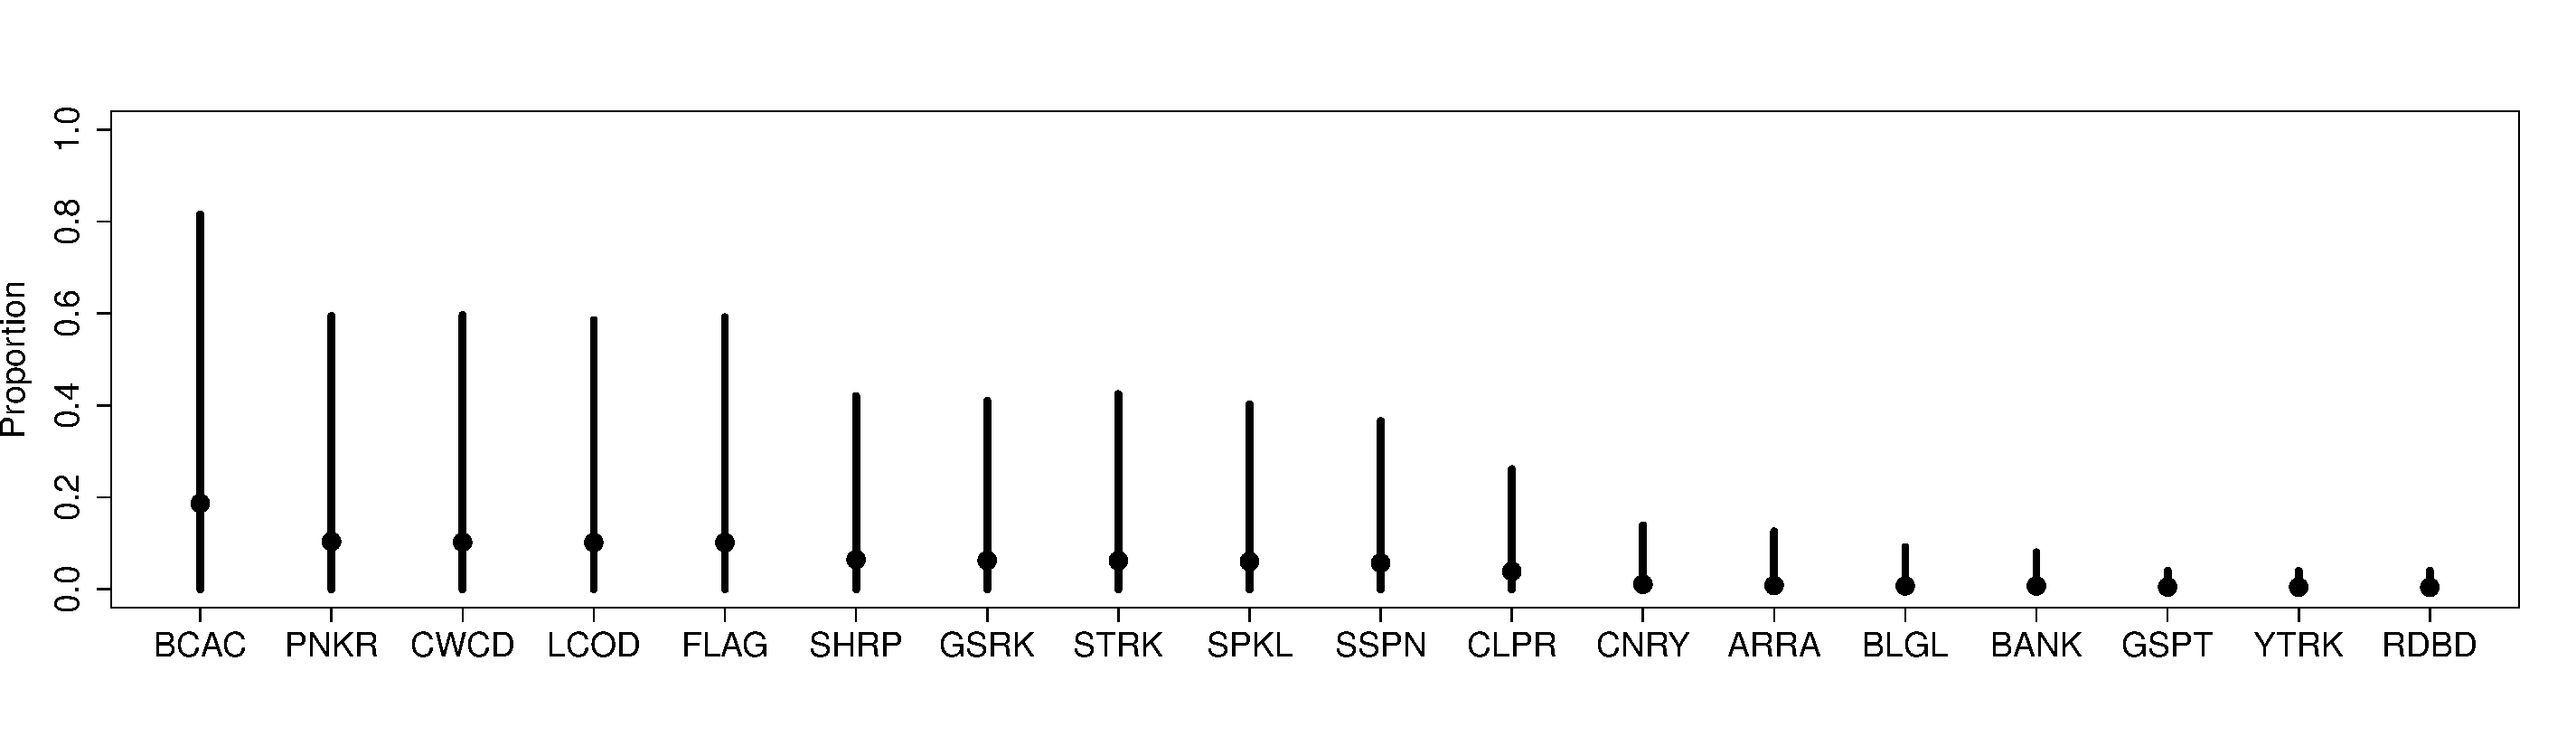
\includegraphics[width=1.15\textwidth]{bocBox1.pdf}
%%
%%$~$\\
%%\vspace{-0.5cm}
%%\begin{minipage}[h!]{0.49\textwidth}
%%$~$\\$~$\\
%%\scalebox{0.8}{\parbox{0.5\linewidth}{
%%\begin{align*}
%%       \text{[1]} ~~ \text{WAIC}       &= -2 f_{WAIC} + 2 p_{WAIC}\\
%%        f_{\text{WAIC}}                        &= \log \prod_{i=1}^{n}{\color{blue}p(y^*=y_i|\bm{y})}\\
%%       p_{\text{WAIC}}                 &= \sum_{i=1}^{n} {\color{blue}\text{Var}_{\bm{\theta}|\bm{y}}\Big( \log p(y_i|\bm{\theta}) \Big)} 
%%\end{align*}
%%}}
%%%\vrule height \vsize \kern 1mm \vrule height \vsize height 2pt 
%%\hspace*{0.1cm}
%%%\vrule{}
%%%\hspace*{-5pt}
%%%\vrule{}
%%\end{minipage}
%%\begin{minipage}[h!]{0.49\textwidth}
%%$~$\\$~$\\$~$\\
%%\end{minipage}
%%$~$\\
%%\vspace{0.1cm}
%%\fontsize{5pt}{7.2}\selectfont
%%%[1] Andrew Gelman, Jessica Hwang, and Aki Vehtari. Understanding predictive information criteria for Bayesian models. \textit{Statistics and Computing}, 24(6):997–1016, 2014.
%%%
%%[1]Gelman, A., Hwang, J., and Vehtari, A. (2014). Understanding predictive information criteria for Bayesian models. \textit{Statistics and Computing,} 24(6), 997-1016.
%%
%%$~$\\$~$\\
%%[2] Jaynes, E. T. (2003). \textit{Probability theory: the logic of science.} Cambridge university press.
%\end{frame}
%
%%
%%
%
%\subsection{}
%\begin{frame}{Port Pooling}%Borrowing Strategies}%How to Tell the old/new story: How to try all partitions and see what happens; (Bias/Variance Trade-off)}
%%0.24
%\hspace{0.5cm}
%\begin{minipage}[h!]{0.2\textwidth}
%        \hspace*{-0.5cm}
%        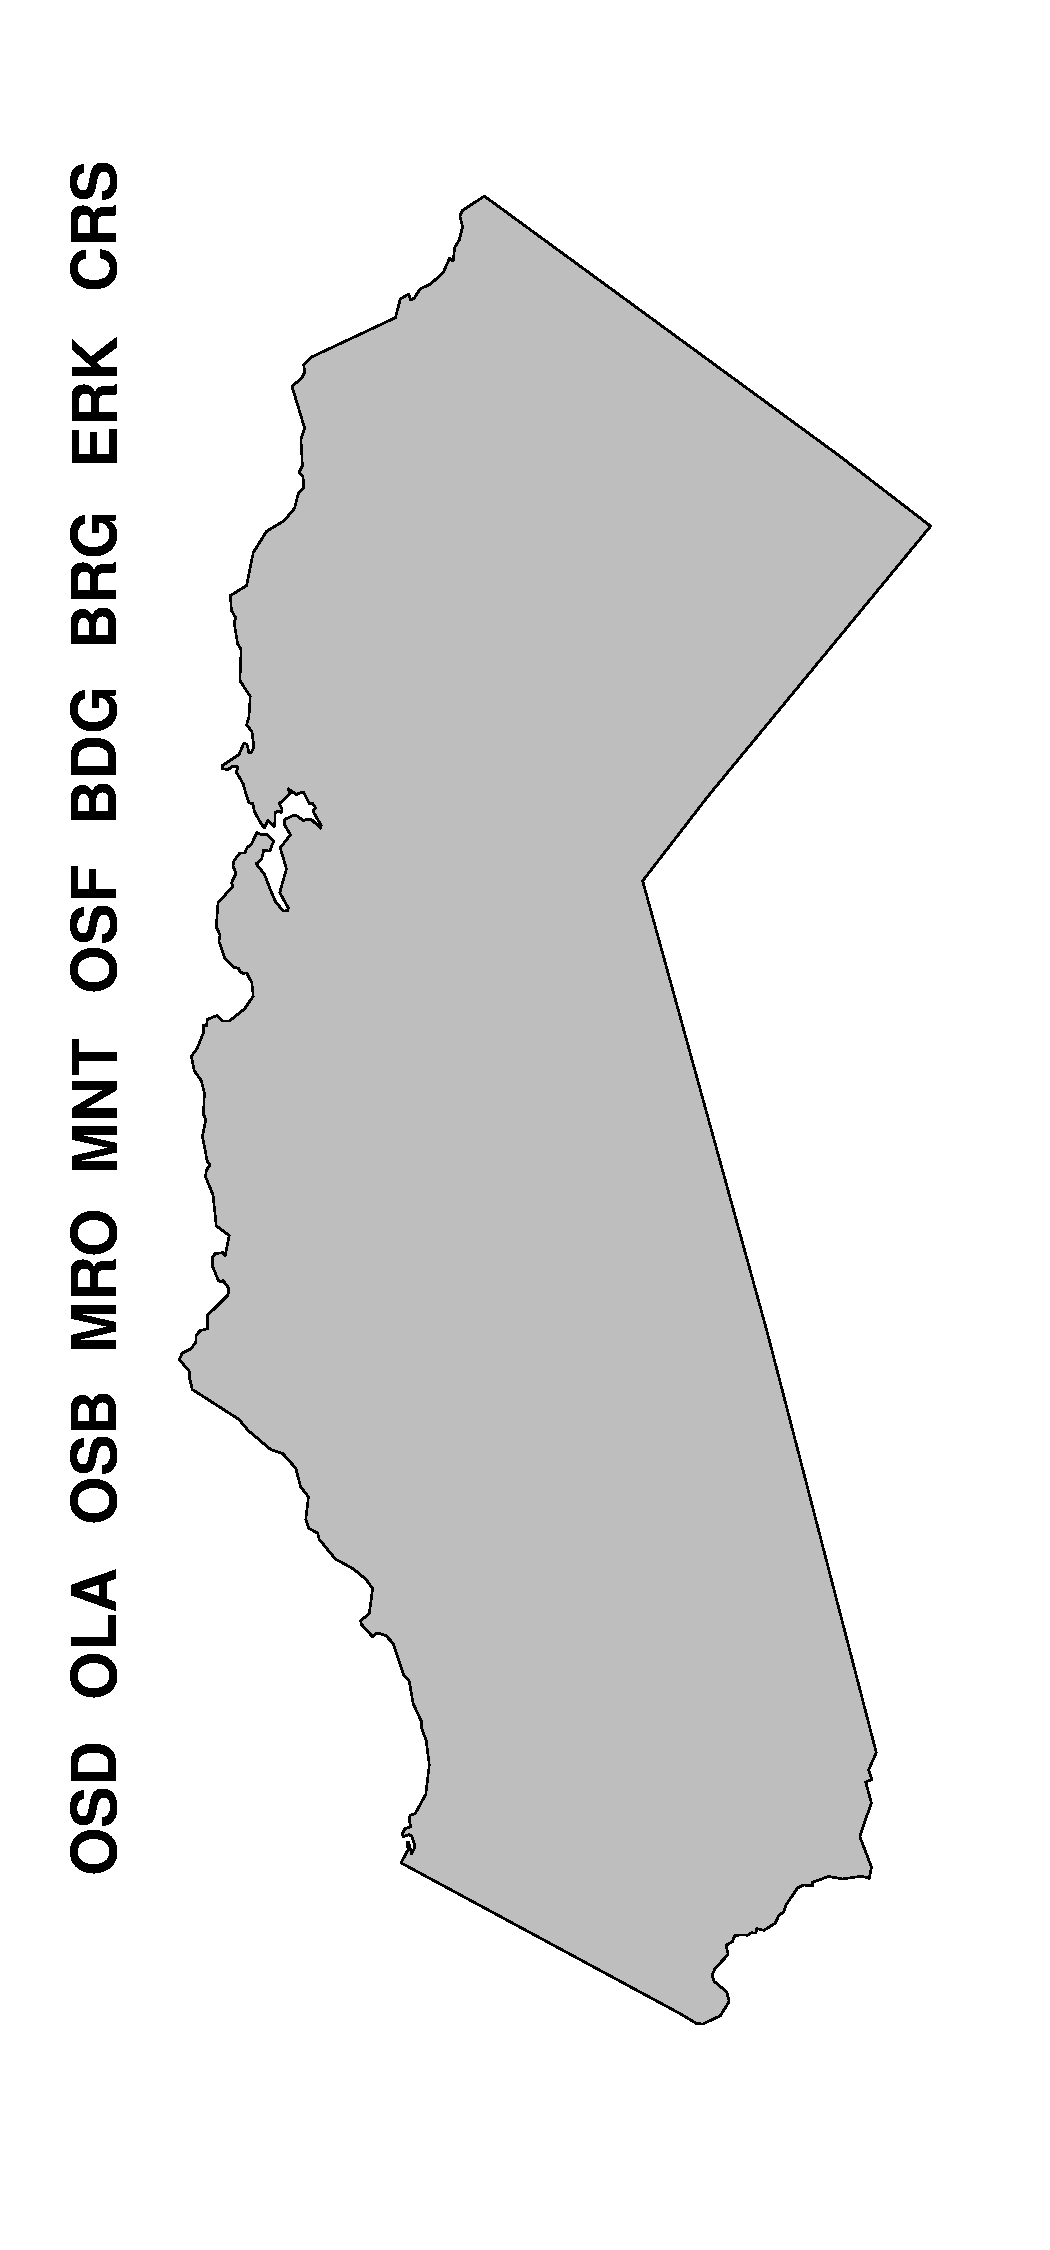
\includegraphics[width=1.2\textwidth]{mapFullBlank.pdf}
%\end{minipage}
%\begin{minipage}[h!]{0.2\textwidth}
%        \hspace*{-0.25cm}
%        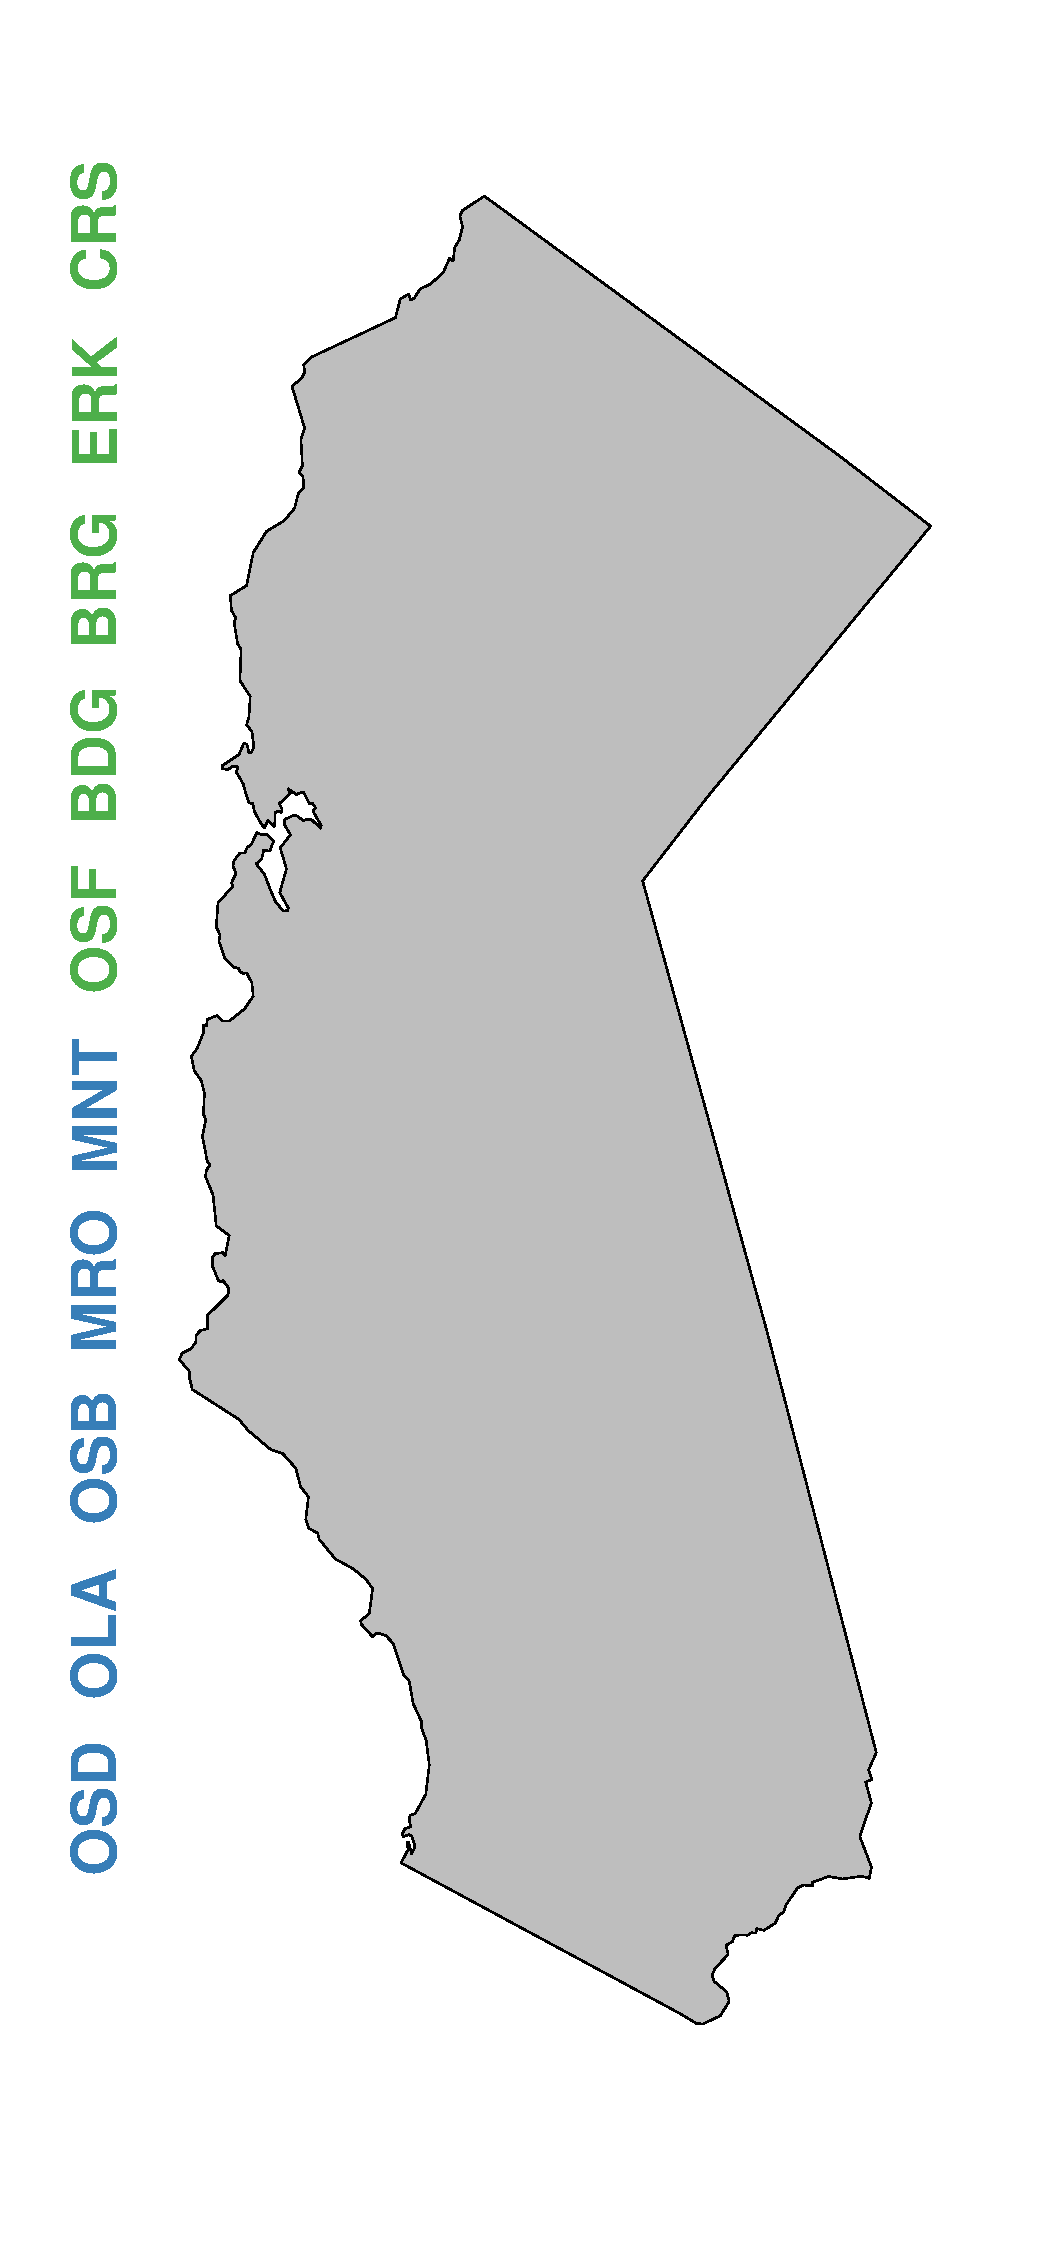
\includegraphics[width=1.2\textwidth]{mapFullHalfHalf.pdf}
%\end{minipage}
%\begin{minipage}[h!]{0.2\textwidth}
%        \hspace*{0.25cm}
%        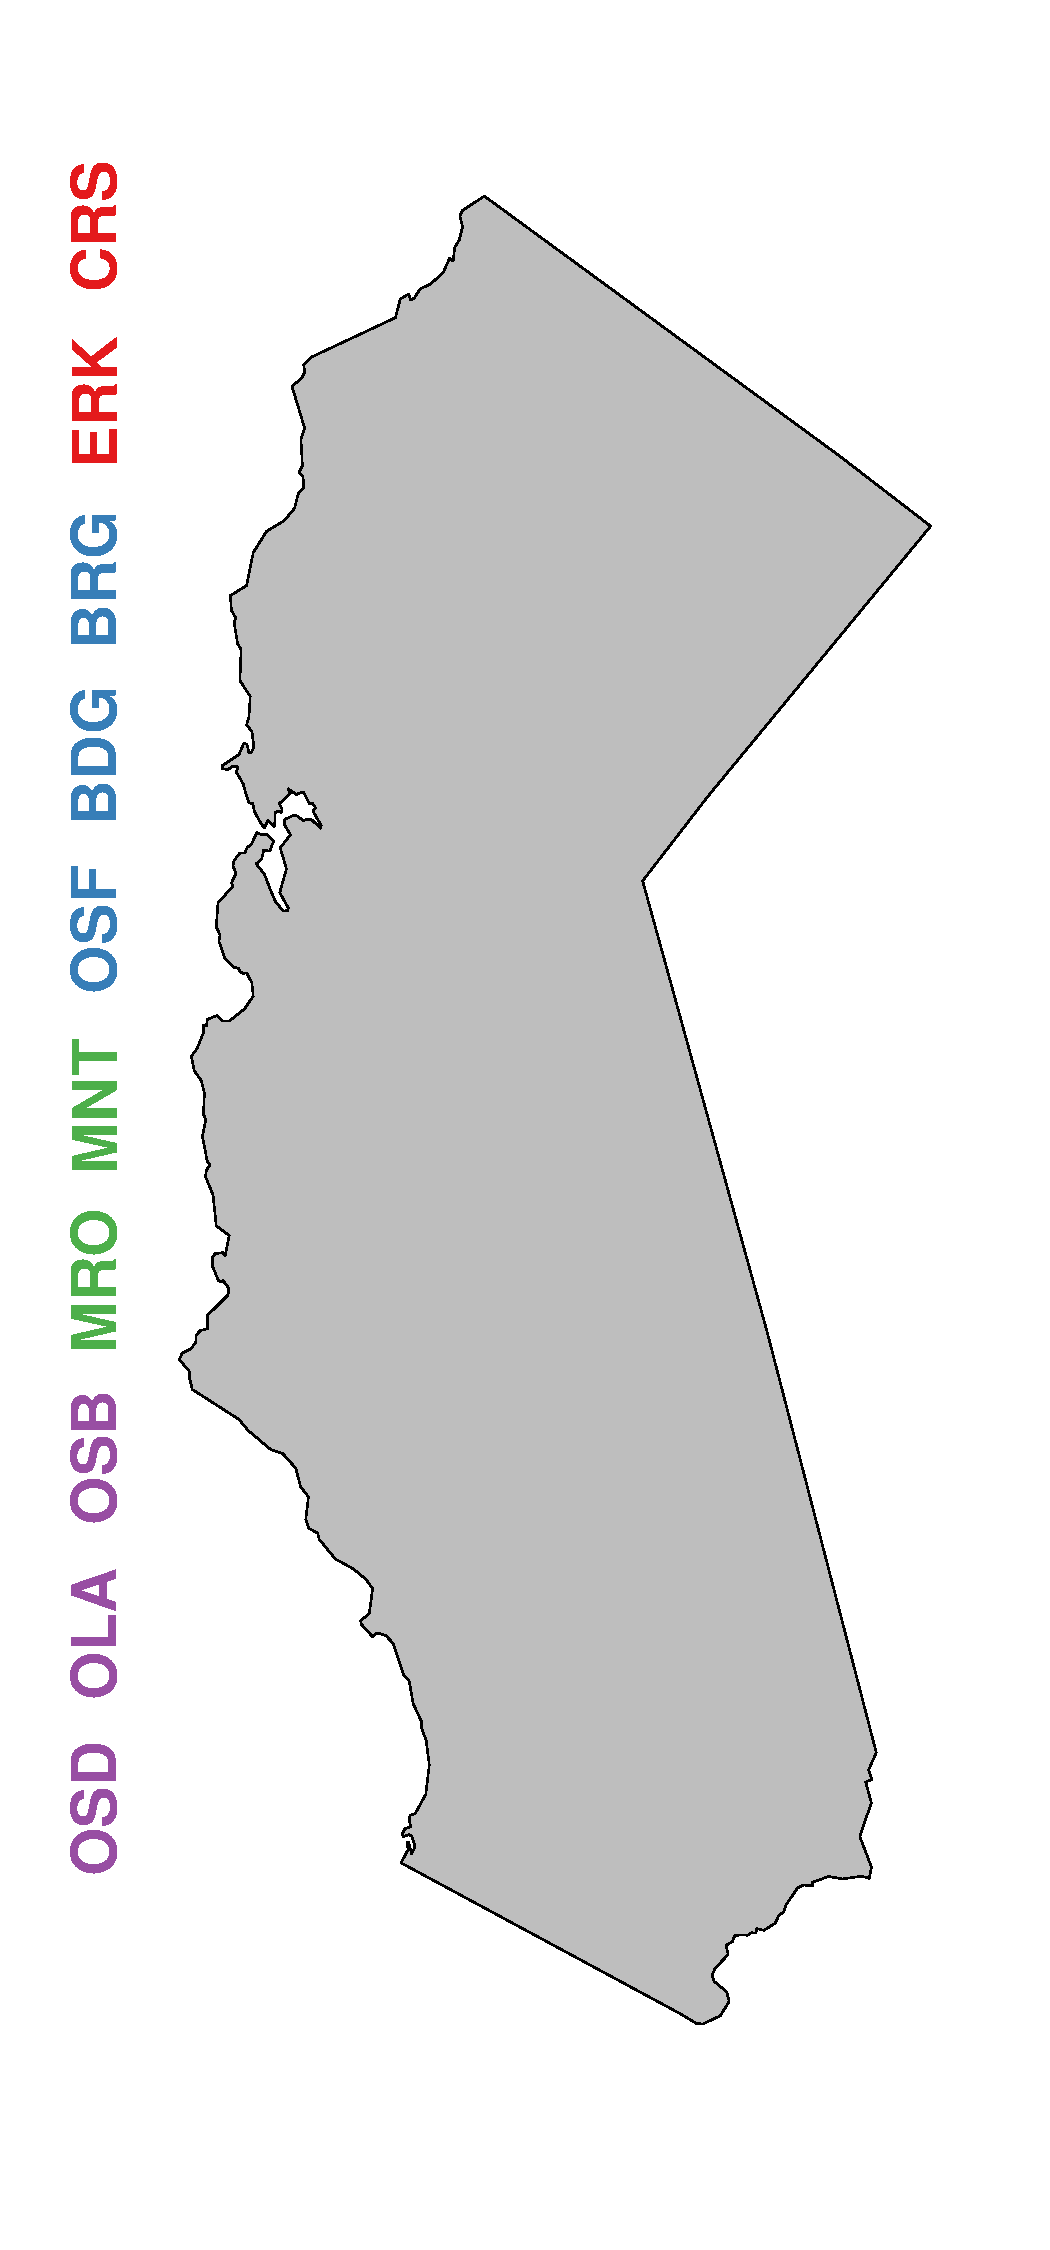
\includegraphics[width=1.2\textwidth]{mapFullConcMend.pdf}
%\end{minipage}
%%\begin{minipage}[h!]{0.19\textwidth}
%%        \hspace*{0.25cm}
%%        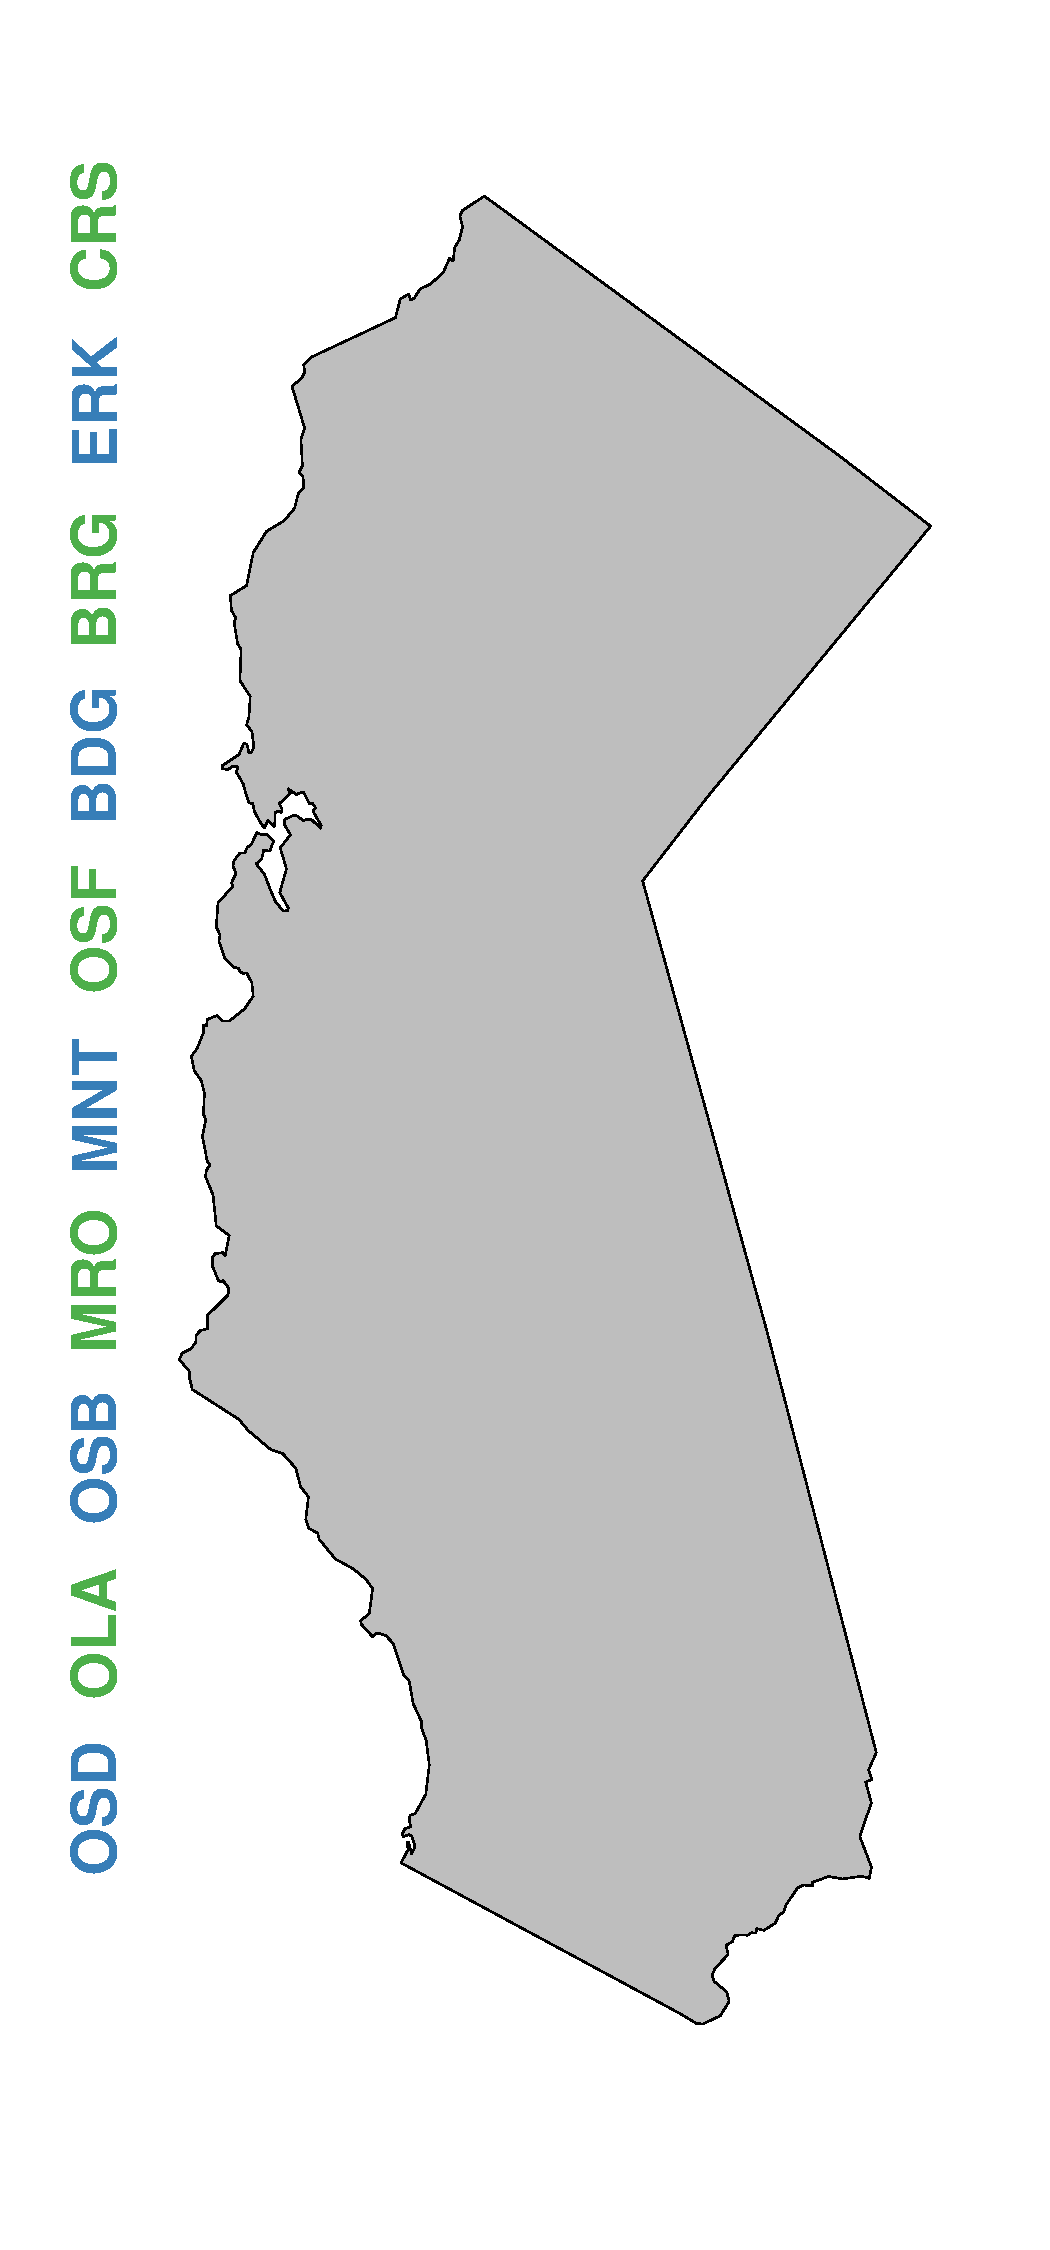
\includegraphics[width=1.2\textwidth]{mapFullEveryOther.pdf}
%%\end{minipage}
%\begin{minipage}[h!]{0.2\textwidth}
%        \hspace*{0.5cm}                %1.2
%        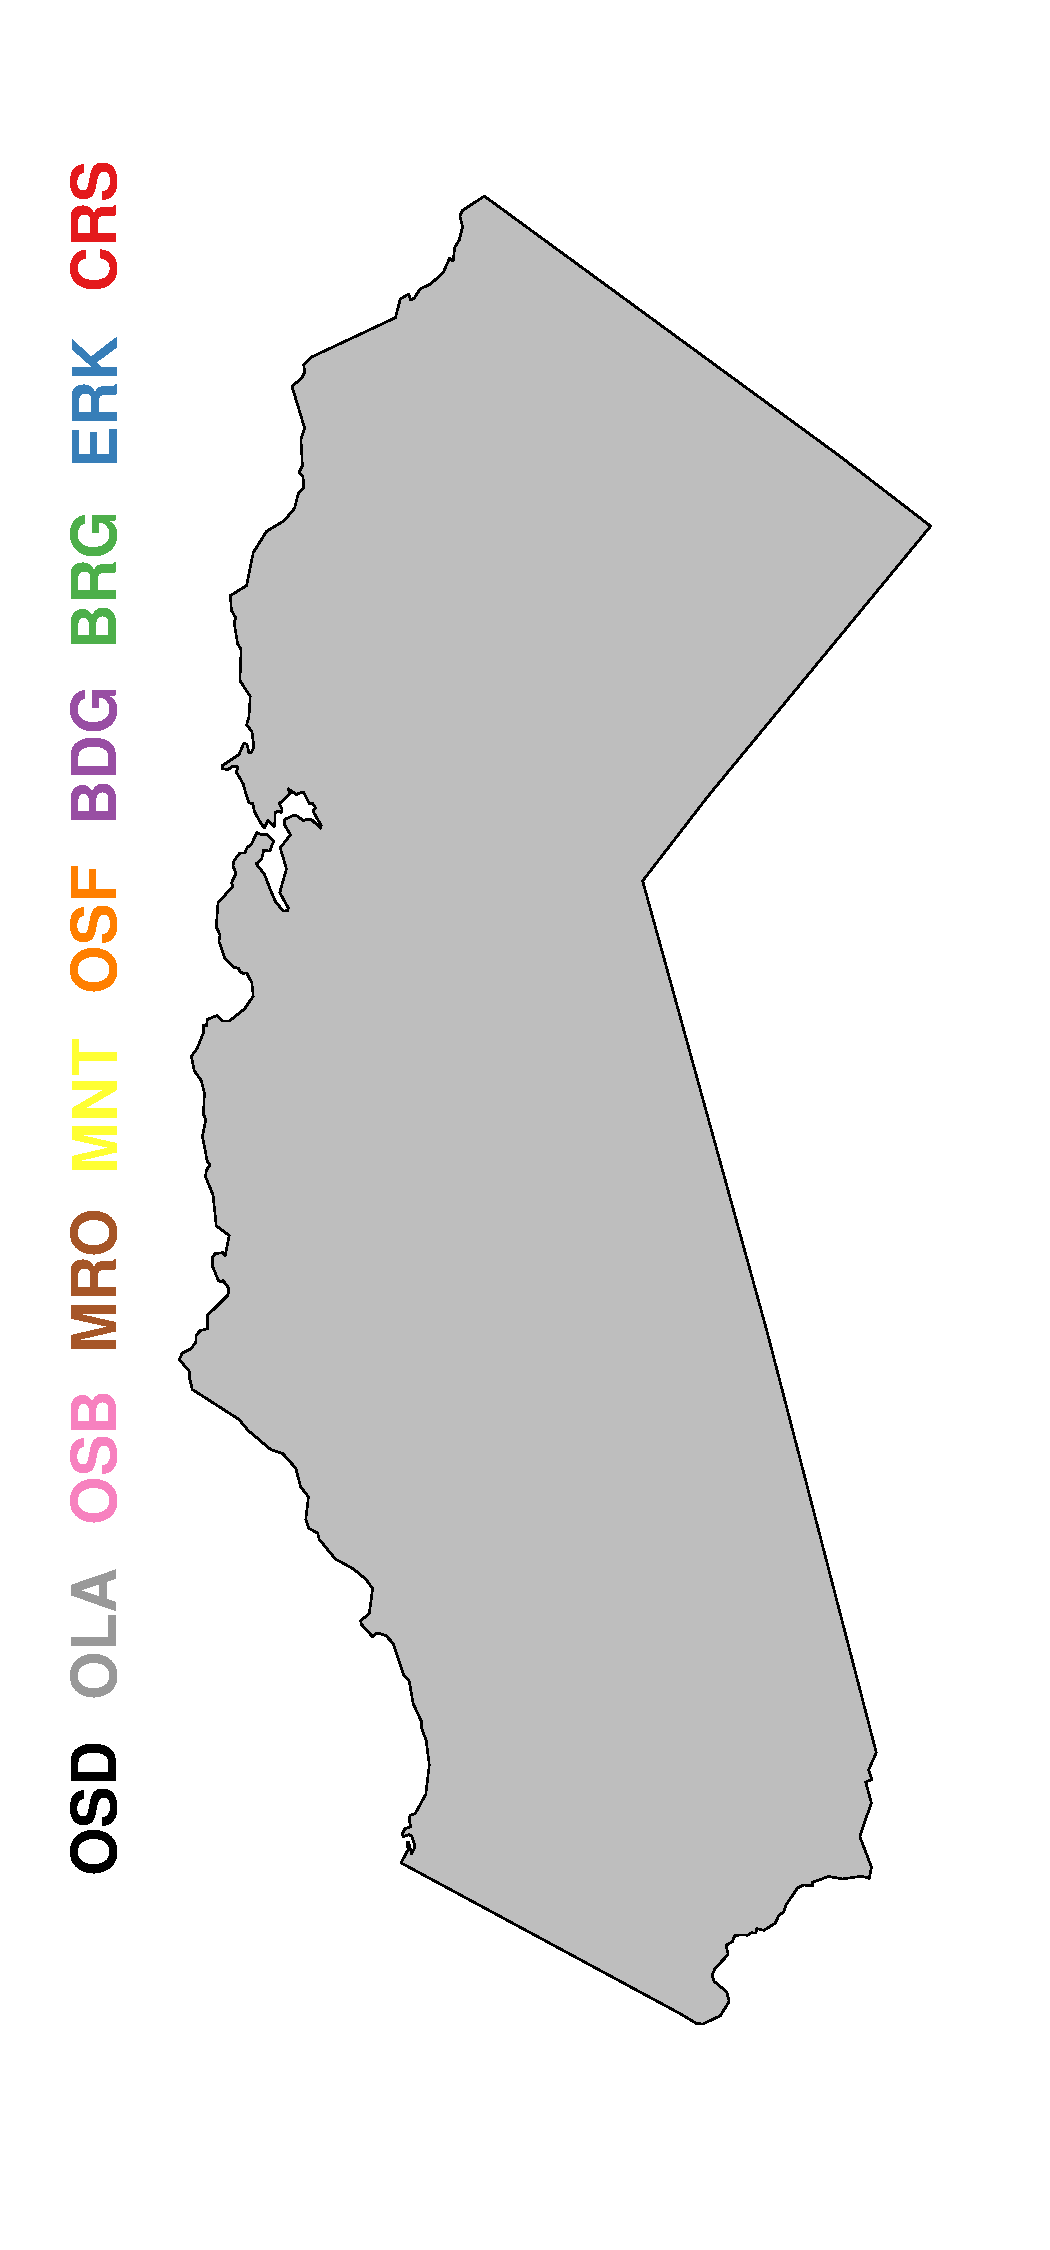
\includegraphics[width=1.2\textwidth]{mapFullSparse.pdf}
%\end{minipage}
%\vspace{-0.5cm}
%\begin{equation*}
%\text{MSE}(\hat\theta) = \mathbb{E}\left[~(\hat\theta - \theta)^2~\right] = \overbrace{\mathbb{E}\Big[~\left(\hat\theta-\mathbb{E}(\hat\theta)\right)^2~\Big]}^{\text{Var}(\hat \theta)} + \overbrace{\Big(~\mathbb{E}(\hat\theta)-\theta~\Big)^2}^{\text{Bias}(\hat \theta, \theta)^2}
%\end{equation*}
%\end{frame}
%
%
%%
%%
%
%%
%%\subsection{}
%\begin{frame}{Bayesian Model Averaging (BMA)}
%      	Consider $j\in \{1, ..., \mathcal{M}\}$ Models ($\mathbb{M}$): % sharing a common distribution $f(y|\bm{\theta})$:
%      	\begin{equation*}
%      	\omega_j = Pr(\mathbb{M}_j|\bm{y}) = \frac{ p(\bm{y}|\mathbb{M}_j)p\cancelto{\propto 1}{(\mathbb{M}_j)} }{ \sum_i p(\bm{y}|\mathbb{M}_i)p\cancelto{\propto 1}{(\mathbb{M}_i)}} = \frac{ p(\bm{y}|\mathbb{M}_j) }{ \sum_i p(\bm{y}|\mathbb{M}_i)}
%	\end{equation*}
%      	\begin{equation*}
%      	\bar p(\bm{\theta}|\bm{y}) = \sum_{j=1}^{\mathcal{M}} \omega_j p(\bm{\theta}|\bm{y}, \mathbb{M}_j)
%      	\end{equation*}
%	\indent if $f$ only depends on $\mathbb{M}$ thru $\bm{\theta}$, then
%      	\begin{equation*}
%      	\bar p(y^*|\bm{y}) = \bm{\int} f(y^*|\bm{\theta}) \bar p(\bm{\theta}|\bm{y}) \bm{d\theta}
%      	\end{equation*}
%$~$\\
%\fontsize{6pt}{7.2}\selectfont
%* Hoeting, J. A., Madigan, D., Raftery, A. E., and Volinsky, C. T. (1999). Bayesian model averaging: a tutorial. \textit{Statistical science}, 382-401.
%
%\end{frame}
%
%%
%%
%
%%
%%\subsection{}
%\begin{frame}{}%{\color{red}ITH} Southern California\color{red}Model Selection Example (Weights, WAIC) $\rightarrow$ look for point conception}
%$~$\\
%%\vspace{-0.5cm}
%\hspace*{-1cm}
%\includegraphics[width=0.6\textwidth]{northern269.pdf}
%\includegraphics[width=0.6\textwidth]{southern269.pdf}\\
%\vspace{-0.5cm}
%\hspace*{-0.3cm}
%\includegraphics[height=0.37\textheight]{./space10MapTop.pdf}
%\includegraphics[height=0.37\textheight]{./space9MapTop.pdf}
%\includegraphics[height=0.37\textheight]{./space14MapTop.pdf}
%\includegraphics[height=0.37\textheight]{./space4MapTop.pdf}
%\hspace*{0.9cm}
%\includegraphics[height=0.37\textheight]{./space2MapBottom.pdf}
%\includegraphics[height=0.37\textheight]{./space4MapBottom.pdf}
%\includegraphics[height=0.37\textheight]{./space5MapBottom.pdf}
%\includegraphics[height=0.37\textheight]{./space1MapBottom.pdf}
%\end{frame}
%
%%
%%
%
%%
%\subsection{}
%\begin{frame}{Expansion and Integration}
%If $\lambda_{\cdot klm\eta\omega}$ is the observed landings of \textbf{all species} in the $k^{th}$ port, caught with the $l^{th}$ gear, in the $\eta^{th}$ quarter, of year $m$, in \mbox{market category $\omega^{th}$}. Then,
%%\begin{equation*}
%%	\lambda^*_{jklm\eta\omega}=\lambda_{\cdot k l m \eta \omega}\pi^*_{jklm\eta\omega}
%%\end{equation*}
%\begin{align*}
%	\lambda^*_{jklm\eta\omega} &=\lambda_{\cdot k l m \eta \omega}\pi^*_{jklm\eta\omega}\\[10pt]
%	\lambda^*_{jklm\eta\cdot} &=\sum_{\omega}\lambda^*_{jklm\eta\omega}\\
%	\lambda^*_{jklm\cdot\cdot} &=\sum_{\eta}\sum_{\omega}\lambda^*_{jklm\eta\omega}\\
%	\lambda^*_{j\cdot lm\cdot\cdot} &=\sum_{k}\sum_{\eta}\sum_{\omega}\lambda^*_{jklm\eta\omega}\\
%	\lambda^*_{j\cdot\cdot m\cdot\cdot} &=\sum_{l}\sum_{k}\sum_{\eta}\sum_{\omega}\lambda^*_{jklm\eta\omega}
%\end{align*}
%\end{frame}
%
%
%
%%
%%
%
%%
%%\subsection{}
%\begin{frame}{$\lambda^*_{j\cdot lm\cdot\cdot}~:~j=\text{Boccaccio}$ }%{\color{red}Post-ITH (require landings)} Landings Thru Time \color{red} Boccaccio time lines for particular gear and port for a couple MCAT}
%	\hspace*{-0.6cm}  %0.59
%	\includegraphics[width=0.55\textwidth]{./TWLLine.pdf}
%	\includegraphics[width=0.55\textwidth]{./OTHLine.pdf}\\
%	\hspace*{-0.6cm}
%	\includegraphics[width=0.55\textwidth]{./HKLLine.pdf}
%	\includegraphics[width=0.55\textwidth]{./NETLine.pdf}	
%\end{frame}
%
%%
%%
%
%%
%\begin{frame}{$\lambda^*_{j\cdot\cdot m\cdot\cdot}~:~j=\text{Boccaccio}$}%{\color{red}Post-ITH (require landings)} Landings Thru Time \color{red} Boccaccio time lines for particular gear and port for a couple MCAT}
%	\vspace{-0.5cm}
%	\hspace*{-1cm}
%	\includegraphics[width=1.2\textwidth]{./gearLine.pdf}
%	%\includegraphics[width=0.59\textwidth]{./OTHLine.pdf}\\
%	%\hspace*{-1cm}
%	%\includegraphics[width=0.59\textwidth]{./HKLLine.pdf}
%	%\includegraphics[width=0.59\textwidth]{./NETLine.pdf}	
%\end{frame}
%
%%
%%
%
%%
%\section{}
%%\subsection{}
%\begin{frame}{Combinatorics}
%%
%\vspace{-0.5cm}
%\hspace{-0.5cm}
%\begin{minipage}[h!]{0.49\textwidth}
%Bell Number: Total number of ways to partition $K$ items.
%\\
%\begin{equation*}
%B_K=\sum_{\hat k=0}^{K} \frac{1}{\hat k!} \left( \sum_{j=0}^{\hat k} (-1)^{\hat k -j} \left(\substack{\hat k \\ j}\right) j^K \right)
%\end{equation*}
%\\
%\mbox{Define $T_0(K)$: Number of ways} to partition $K$ items, such that, partitions are adjacent. % (spatially/temporally).
%\end{minipage}
%\begin{minipage}[h!]{0.49\textwidth}
%        \hspace{0.7cm}
%	%\vspace{5cm}
%        \includegraphics[width=1\textwidth]{constModelsSim.pdf}
%\end{minipage}
%\includegraphics[width=1\textwidth]{constB4.pdf}
%%
%\end{frame}
%
%%
%%
%
%%
%\usebackgroundtemplate{\tikz\node[opacity=0.6]{\hspace*{-0.12cm}\includegraphics[width=\paperwidth]{tiledRedFish.png}};}
%\begin{frame}
%\titlepage
%\end{frame}
%\usebackgroundtemplate{}

\end{document}
